% opx_architecture.tex -- the ARTIQ <-> Quantum Machines OPX+ integration of
% the K-machine (kexp) codebase, written for a physicist who knows ARTIQ but
% not QUA. Build: latexmk -pdf opx_architecture.tex (see README.md).
%
% Conservative LaTeX on purpose: article class, the packages below only, TikZ
% drawn with plain \draw/\node/\fill (no tikz-timing, no pgfplots). No TeX
% toolchain was available where this was written, so the file was checked
% for environment/brace balance by script only -- if a compile error shows
% up, it is a typo, not a missing package.

\documentclass[11pt,a4paper]{article}

\usepackage[T1]{fontenc}
\usepackage[utf8]{inputenc}
\usepackage{amsmath}
\usepackage{amssymb}
\usepackage[margin=2.3cm]{geometry}
\usepackage{booktabs}
\usepackage{listings}
\usepackage{xcolor}
\usepackage{tikz}
\usepackage{enumitem}
\usepackage[colorlinks=true,linkcolor=blue!50!black,urlcolor=blue!50!black,citecolor=blue!50!black]{hyperref}

% ---------------------------------------------------------------------------
% macros
% ---------------------------------------------------------------------------
\newcommand{\code}[1]{\texttt{#1}}
\newcommand{\file}[1]{\texttt{#1}}
\newcommand{\planned}{\textcolor{red!70!black}{\textbf{[planned]}}}
\newcommand{\micro}{\ensuremath{\mu}}
\newcommand{\us}{\ensuremath{\,\mu\mathrm{s}}}
\newcommand{\nsu}{\ensuremath{\,\mathrm{ns}}}
\newcommand{\cc}{\ensuremath{\,\mathrm{cc}}}

% a plain framed box for status / warnings (no extra packages)
\newcommand{\statusbox}[2]{%
  \noindent\fbox{\begin{minipage}{\dimexpr\linewidth-2\fboxsep-2\fboxrule\relax}%
  \textbf{#1}\quad #2%
  \end{minipage}}\par\medskip}

% ---------------------------------------------------------------------------
% listings
% ---------------------------------------------------------------------------
\definecolor{lstbg}{gray}{0.96}
\definecolor{lstcomment}{rgb}{0.35,0.45,0.35}
\definecolor{lstkw}{rgb}{0.10,0.20,0.60}
\lstset{
  basicstyle=\small\ttfamily,
  backgroundcolor=\color{lstbg},
  columns=fullflexible,
  keepspaces=true,
  breaklines=true,
  breakatwhitespace=true,
  frame=single,
  framerule=0.2pt,
  xleftmargin=4pt,
  xrightmargin=4pt,
  showstringspaces=false,
  tabsize=4,
  commentstyle=\color{lstcomment}\itshape,
  keywordstyle=\color{lstkw}\bfseries,
  stringstyle=\color{black},
  numbers=none,
}
\lstdefinestyle{py}{language=Python}
\lstdefinestyle{qua}{language=Python}
\lstdefinestyle{txt}{language={},basicstyle=\scriptsize\ttfamily,commentstyle=\ttfamily,keywordstyle=\ttfamily}

% ---------------------------------------------------------------------------
\title{Two controllers, one shot:\\
  the ARTIQ\,$\leftrightarrow$\,OPX+ integration of the K-machine codebase\\[1ex]
  \large \file{kexp.control.opx}, the handshake kernels, the data path,\\
  and the on-OPX Bayesian feedback port}
\author{Weld lab, K-39 experiment\\
  \small documentation written 2026-09-24 against the phase-2 rebuild (design spec of the same day);\\
  \small feedback section updated 2026-09-25 to the speed pass ``3b''}
\date{}

\begin{document}
\maketitle

\statusbox{Status.}{%
This document describes the OPX integration \emph{as it exists after the
phase-2 rebuild} (the design spec of 2026-09-24: framework fixes in
\file{kexp/control/opx}, the config-time parameter guard, the component
layer, the context additions, and the Bayesian-feedback port), with the
feedback port as of its speed pass ``3b'' (2026-09-25: argmax control law,
grid-index drive with exact integer-Hz IFs, co-rotating frame, $L/32$ log
weights, sine table, optional discrete durations). Everything in it has been
\textbf{offline-tested only}: traced with the qm-qua DSL, checked by 126 unit
tests (\file{test\_opx.py} 39, \file{test\_opx\_ctx.py} 24,
\file{test\_opx\_config.py} 19, \file{test\_opx\_viewer.py} 8,
\file{opx\_sim\_fixture.py} 8, \file{test\_feedback\_opx.py} 28) and, for the
feedback port, compiled and timed on the QOP simulator (7.75\us\ of compute
per pulse for $m = 21$). \textbf{No part of this design has run against
atoms.} The hardware milestones M1--M4 (appendix~\ref{sec:milestones}) are
open; M4 is needed only for the remesh. One item is a design, not code: the
remesh with pole return (section~\ref{sec:feedback:remesh}), marked
\planned. Every number quoted is the value in the code, the parameter file or
the simulator record on the date of its section, with the file named where
it matters.}

\tableofcontents
\clearpage

\section*{How to read this}
\addcontentsline{toc}{section}{How to read this}

You know ARTIQ: the RTIO timeline, \code{delay()}, \code{now\_mu()}, kernels
compiled for the Kasli core device, RPCs to the host, and the lab's
\code{Base}/\code{scan\_kernel}/\code{xvar} conventions. You may not know QUA,
the language of the Quantum Machines OPX+. This document tries to teach the
integration \emph{by mechanism}: every diagram shows what the code actually
emits or schedules, with the real numbers, and every claim names its file.
Sections~\ref{sec:why}--\ref{sec:handoff} are the framework as a whole,
\ref{sec:data}--\ref{sec:midloop} are the data and parameter plumbing,
\ref{sec:tutorial} is a tutorial for writing a new per-shot sequence,
\ref{sec:quam} maps our objects onto QUA's own abstraction layer (QUAM),
and \ref{sec:feedback} is the Bayesian feedback loop ported to run on the OPX,
with its timing, numerics and speed work, and the planned remesh.

Two vocabulary notes up front. A \emph{shot} is one ARTIQ \code{scan\_kernel}
iteration; on the OPX it is one iteration of the program's shot loop, and the
two are tied together by exactly one trigger per shot. A \emph{sequence} is
the OPX-side body of one shot, written as a Python function traced once into
QUA (section~\ref{sec:program}).

\section{Why two controllers}
\label{sec:why}

\subsection{What ARTIQ is good at, and what it is not}

ARTIQ schedules \emph{events} on a timeline. A kernel running on the Kasli
core device writes RTIO output events (a TTL edge, a DDS register write, a
DAC value) with a timestamp in machine units (1\,mu = 1\nsu\ on this
machine, coarse clock 8\nsu)\footnote{\file{k-exp/kexp/util/db/device\_db.py}
(\code{ref\_period = 1e-9}); \code{t\_rtio = 8e-9} in
\file{kexp/config/expt\_params.py}.}, and the gateware plays them out
deterministically. The kernel CPU (a soft core) does the bookkeeping: it
runs the Python-compiled control flow, submits events into FIFOs ahead of
real time, and blocks on input events (\code{timestamp\_mu}). Two consequences
matter here:

\begin{itemize}[nosep]
  \item Output timing is exact to the coarse clock, \emph{as long as the CPU
    stays ahead}. If an event is submitted after its timestamp has passed, the
    kernel raises \code{RTIOUnderflow}. The lab's scan loop catches it and
    aborts the run (section~\ref{sec:handoff:crash}).
  \item Real-time \emph{computation} is slow. The Bayesian feedback loop of
    section~\ref{sec:feedback} runs a 21-point posterior update on the kernel
    CPU in double precision; the budget reserved for it is
    \code{t\_calculation\_slack\_compensation\_mu} $= 0.7\us\times m + 15\us =
    29.7\us$ for $m = 21$, plus an 18.4\us\ ``fifo'' allowance, so each
    feedback cycle is 57--61\us\ long for 10--14\us\ of physics.\footnote{\file{k-exp/kexp/experiments/HF\_experiments/feedback/expt\_params\_feedback.py},
    lines 79--81; \file{k-exp/kexp/base/feedback.py}, \code{compute\_t\_between\_pulses\_mu}.}
    The reading of the analog integrator through the Sampler is itself a
    blocking SPI transaction that leaves ``slack $\sim$zero'' on return.
\end{itemize}

\subsection{What the OPX+ is good at}

The Quantum Machines OPX+ is a pulse processor: 18 real-time cores, each
owning one \emph{element} (a logical channel bound to analog/digital ports),
running a compiled QUA program in lock-step at a 4\nsu\ clock cycle
(cc).\footnote{\file{k-exp/kexp/control/opx/units.py}: \code{CLOCK\_NS = 4},
\code{MIN\_PULSE\_CC = 4}.} Its strengths, relative to ARTIQ, are:

\begin{itemize}[nosep]
  \item \textbf{Real-time arithmetic next to the pulses.} QUA has 32-bit
    integers and 4.28 fixed-point reals (range $[-8, 8)$, step $2^{-28}$),
    a \code{Math} library (\code{sqrt}, \code{inv}, \code{exp}, \code{cos2pi},
    \code{sin2pi}, whole-array \code{sum}/\code{max}/\code{argmax}/\code{dot}),
    and a \code{measure} statement whose integrated result is usable by the
    next statement. The posterior update becomes a few microseconds of
    fixed-point work interleaved with the pulses, not tens of microseconds of
    soft-CPU floating point.
  \item \textbf{Deterministic timing by construction.} A statement whose
    inputs are known at compile time is scheduled without gaps; a statement
    that depends on a QUA variable adds ``a few cycles''. Either way the
    element clock advances by exactly the durations played and waited, which
    is what section~\ref{sec:feedback} relies on.
  \item \textbf{Sticky elements} (section~\ref{sec:why:sticky}) hold an
    analog level or a digital marker across statements, so a CW tone or a
    switch level is set once and stays.
  \item \textbf{Streams} carry measurement results and timestamps back to the
    host asynchronously, without stalling the program.
\end{itemize}

What the OPX+ does \emph{not} do for us: it has no shutters, no coils, no
camera, no line trigger, no 200-parameter experiment object. The MOT, the
tweezer loading, the shutters, the field, the imaging and every other part of
the shot stay on ARTIQ. The OPX is handed the atoms for one window per shot
(section~\ref{sec:handoff}) and hands them back.

\subsection{The wires}
\label{sec:why:wires}

Figure~\ref{fig:wires} shows every physical connection the integration uses.
There are three logic wires between the two controllers and four beam-path
connections.

\begin{figure}[htbp]
\centering
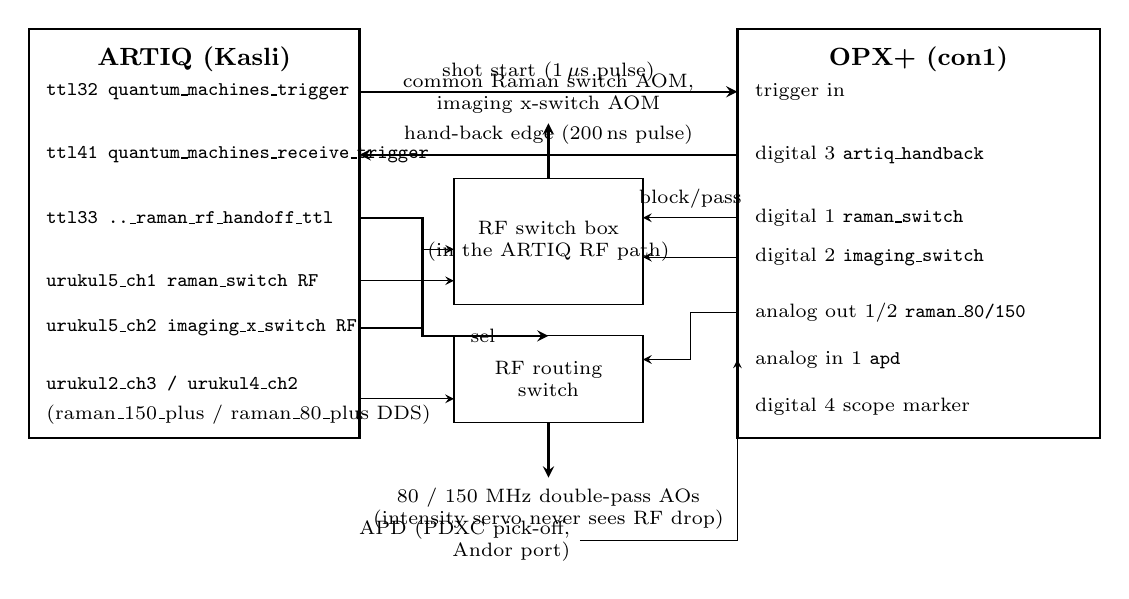
\begin{tikzpicture}[>=stealth, font=\small, x=1cm, y=1cm]
  % ARTIQ box
  \draw[thick] (0,0) rectangle (4.2,5.2);
  \node[anchor=north] at (2.1,5.1) {\textbf{ARTIQ (Kasli)}};
  \node[anchor=west, font=\scriptsize\ttfamily] at (0.1,4.4) {ttl32 quantum\_machines\_trigger};
  \node[anchor=west, font=\scriptsize\ttfamily] at (0.1,3.6) {ttl41 quantum\_machines\_receive\_trigger};
  \node[anchor=west, font=\scriptsize\ttfamily] at (0.1,2.8) {ttl33 ..\_raman\_rf\_handoff\_ttl};
  \node[anchor=west, font=\scriptsize\ttfamily] at (0.1,2.0) {urukul5\_ch1 raman\_switch RF};
  \node[anchor=west, font=\scriptsize\ttfamily] at (0.1,1.4) {urukul5\_ch2 imaging\_x\_switch RF};
  \node[anchor=west, font=\scriptsize\ttfamily] at (0.1,0.7) {urukul2\_ch3 / urukul4\_ch2};
  \node[anchor=west, font=\scriptsize] at (0.1,0.3) {(raman\_150\_plus / raman\_80\_plus DDS)};
  % OPX box
  \draw[thick] (9.0,0) rectangle (13.6,5.2);
  \node[anchor=north] at (11.3,5.1) {\textbf{OPX+ (con1)}};
  \node[anchor=west, font=\scriptsize] at (9.1,4.4) {trigger in};
  \node[anchor=west, font=\scriptsize] at (9.1,3.6) {digital 3 \code{artiq\_handback}};
  \node[anchor=west, font=\scriptsize] at (9.1,2.8) {digital 1 \code{raman\_switch}};
  \node[anchor=west, font=\scriptsize] at (9.1,2.3) {digital 2 \code{imaging\_switch}};
  \node[anchor=west, font=\scriptsize] at (9.1,1.6) {analog out 1/2 \code{raman\_80/150}};
  \node[anchor=west, font=\scriptsize] at (9.1,1.0) {analog in 1 \code{apd}};
  \node[anchor=west, font=\scriptsize] at (9.1,0.4) {digital 4 scope marker};
  % logic wires
  \draw[->, thick] (4.2,4.4) -- (9.0,4.4) node[midway, above, font=\scriptsize] {shot start (1\us\ pulse)};
  \draw[<-, thick] (4.2,3.6) -- (9.0,3.6) node[midway, above, font=\scriptsize] {hand-back edge (200\nsu\ pulse)};
  % RF routing switch
  \draw (5.4,0.2) rectangle (7.8,1.3);
  \node[font=\scriptsize, align=center] at (6.6,0.75) {RF routing\\switch};
  \draw[->, thick] (4.2,2.8) -- (5.0,2.8) -- (5.0,1.3) -- (6.6,1.3) node[pos=0.3, right, font=\scriptsize] {sel};
  \draw[->] (4.2,0.5) -- (5.4,0.5);
  \draw[->] (9.0,1.6) -- (8.4,1.6) -- (8.4,1.0) -- (7.8,1.0);
  \draw[->, thick] (6.6,0.2) -- (6.6,-0.5) node[below, font=\scriptsize, align=center] {80 / 150 MHz double-pass AOs\\(intensity servo never sees RF drop)};
  % RF switch box
  \draw (5.4,1.7) rectangle (7.8,3.3);
  \node[font=\scriptsize, align=center] at (6.6,2.5) {RF switch box\\(in the ARTIQ RF path)};
  \draw[->] (4.2,2.0) -- (5.4,2.0);
  \draw[->] (4.2,1.4) -- (5.0,1.4) -- (5.0,2.4) -- (5.4,2.4);
  \draw[->] (9.0,2.8) -- (7.8,2.8) node[midway, above, font=\scriptsize] {block/pass};
  \draw[->] (9.0,2.3) -- (7.8,2.3);
  \draw[->, thick] (6.6,3.3) -- (6.6,4.0) node[above, font=\scriptsize, align=center] {common Raman switch AOM,\\imaging x-switch AOM};
  % APD
  \draw[->] (7.0,-1.3) -- (9.0,-1.3) -- (9.0,1.0);
  \node[anchor=east, font=\scriptsize, align=right] at (7.0,-1.3) {APD (PDXC pick-off,\\Andor port)};
\end{tikzpicture}
\caption{Every connection the integration uses. Channel names are the
\code{ttl\_frame}/\code{dds\_frame} attributes in
\file{k-exp/kexp/config/ttl\_id.py} (lines 64--66) and
\file{dds\_id.py}; OPX ports are the constants at the top of
\file{k-exp/kexp/control/opx/opx\_config.py}. The RF routing switch and the
RF switch box are the lab's own hardware (2026-09 wiring); the OPX never
sees the AOMs directly except through them.}
\label{fig:wires}
\end{figure}

\paragraph{The three logic wires.}
\begin{enumerate}[nosep]
  \item \code{ttl32} $\to$ OPX trigger input. ARTIQ pulses it for
    \code{T\_OPX\_TRIGGER\_PULSE} $= 1\us$ to start one OPX shot. The OPX
    samples this input at 250\,MHz; QM publishes no trigger-to-output
    latency (milestone M1).\footnote{\file{k-exp/kexp/base/control.py}
    line 34; \file{k-exp/kexp/config/ttl\_id.py} line 65.}
  \item OPX digital 3 (\code{artiq\_handback}) $\to$ \code{ttl41}, a
    \code{TTLInOut} gated for rising edges. The OPX plays a 200\nsu\ pulse
    here when its body is done; ARTIQ's kernel is blocked in
    \code{timestamp\_mu} waiting for it.
  \item \code{ttl33} $\to$ the RF routing switch. High = the 80 and
    150\,MHz double-pass AOs are driven by OPX analog outputs 1 and 2; low =
    by the ARTIQ DDSs \code{raman\_80\_plus}/\code{raman\_150\_plus}.
\end{enumerate}

\paragraph{The beam-path connections.} OPX digital 1 and 2 drive an RF
switch box \emph{in the ARTIQ RF path} of the common Raman switch AOM
(\code{urukul5\_ch1}) and the imaging x-switch AOM (\code{urukul5\_ch2}).
OPX analog 1/2 carry the 80/150\,MHz AO tones during the window. The APD
signal enters OPX analog input 1. Digital 4 is a scope marker played during
every ADC window and does nothing else.

\subsection{The truth table}
\label{sec:why:truth}

\begin{table}[htbp]
\centering
\small
\begin{tabular}{@{}llll@{}}
\toprule
line & level & meaning & who sets it \\
\midrule
OPX digital 1 (\code{raman\_switch}) & HIGH & ARTIQ RF to the Raman switch AOM \textbf{blocked} & OPX op \code{block} \\
 & LOW & RF \textbf{passes} (idle state with no job) & OPX op \code{pass} / no job \\
OPX digital 2 (\code{imaging\_switch}) & HIGH / LOW & same, imaging x-switch AOM & same \\
OPX digital 3 (\code{artiq\_handback}) & rising edge & ``body done, take the beams back'' & OPX op \code{trigger} \\
ARTIQ \code{ttl33} & HIGH & 80/150 AOs driven by OPX analog 1/2 & kernel \\
 & LOW & 80/150 AOs driven by ARTIQ DDSs & kernel, idle \\
ARTIQ \code{urukul5\_ch1/2} switch & ON & steady-state RF offered to the switch box & kernel, only inside the window \\
\bottomrule
\end{tabular}
\caption{Polarity of every line, from the truth table in
\file{k-exp/kexp/control/opx/opx\_config.py} (module docstring and
\code{BLOCK\_LEVEL = 1}). ``Block'' is the high level on purpose: with no
job running the OPX lines idle low, so ARTIQ gates its own light in every
non-OPX run exactly as before.}
\label{tab:truth}
\end{table}

The consequence that shapes the whole handshake: \emph{during an OPX window
ARTIQ turns its switch-AOM RF on steady-state and leaves it on}; the OPX then
makes light by opening (\code{pass}) and closing (\code{block}) the switch
box. An exposure of duration $d$ is literally \code{play('pass', 'raman\_switch',
duration=d)} followed immediately by \code{play('block', 'raman\_switch')}.
Because the switch element is sticky-digital, the line stays low for exactly
$d$ and there is no gap before the re-block.\footnote{\file{k-exp/kexp/control/opx/context.py},
\code{OPXShotContext.\_expose}.}

\subsection{Sticky elements}
\label{sec:why:sticky}

A QUA element declared \code{'sticky': \{'analog': True, 'digital': True,
'duration': ...\}} holds the last analog sample and the last digital marker
level after a pulse ends, until the next pulse on that element overrides it.
Three facts about sticky behaviour drive our design (all from QM's feature
guide, verified offline only):

\begin{enumerate}[nosep]
  \item \textbf{Analog sticky plays \emph{add} to the held value.} Playing a
    latch pulse twice doubles the amplitude. The customer script
    \file{00g\_hello\_atoms\_apd.py} looped three times without a
    \code{ramp\_to\_zero} and would have driven \code{raman\_B} from 0.325\,V to
    0.650\,V on shot 2 (beyond the $\pm 0.5$\,V full scale). This is why the
    builder latches the analog drives \textbf{once per run}, in the program
    prologue, and ramps them to zero once in the epilogue
    (section~\ref{sec:program:skeleton}).
  \item \textbf{Digital sticky needs \code{analog: True}.} The QOP rejects a
    job whose element is digital-sticky but not analog-sticky (``sticky
    digital but analog sticky wasn't set'', seen 2026-09-23). Our switch
    elements have no analog port at all and set \code{analog: True} anyway;
    QM's own template instead gave each gate a dummy analog port. Whether
    the QOP accepts a port-less sticky element is an M1 item.
  \item \textbf{A sticky element ramps back to its DC offset at the end of
    the program}, i.e.\ when the job is halted the lines return to idle (low =
    pass). What the digital lines do on \code{job.halt()} \emph{mid-block} is
    not documented -- M1.
\end{enumerate}

\subsection{Why the analog drives are latched and the switch AOM is gated}

The two Raman beams reach the atoms through the 80 and 150\,MHz double-pass
AOs (one per beam, setting the two-photon frequency) and a \emph{common}
switch AOM (setting the pulse envelope). The double-pass AOs sit inside an
intensity servo that must never see its RF drop; the switch AOM's thermal
load depends on its duty cycle. Hence:

\begin{itemize}[nosep]
  \item The OPX \emph{drives} the 80/150 AOs with sticky CW tones latched
    once per run, at exactly the frequencies \code{prep\_raman()} would have
    programmed on the ARTIQ DDSs (the same \code{RamanBeamPair.ao\_frequencies}
    split, section~\ref{sec:program:config}). The routing switch
    (\code{ttl33}) decides whose tone reaches the AOs; the tone itself never
    stops during the run.
  \item The OPX \emph{gates} the switch AOM by blocking/passing ARTIQ's own
    steady-state RF. The OPX does not synthesise the switch RF and does not
    control its amplitude.
\end{itemize}

\paragraph{Why \code{prep\_raman()} stays.} Before the handoff, ARTIQ still
runs \code{prep\_raman()}: it initialises the \code{RamanBeamPair}, plays a
3\,ms warm-up pulse on the switch AOM \emph{with the shutter still closed},
waits 10\us, opens the Raman shutter (3\,ms), waits for the 60\,Hz line
trigger and adds 4.7\,ms.\footnote{\file{k-exp/kexp/base/control.py},
\code{prep\_raman}, lines 154--182.} The warm-up thermally loads the very
AOM the OPX will gate; the OPX's sticky drives keep only the 80/150 AOs
warm and are no substitute. The shutter and the line-trigger phasing are
ARTIQ hardware the OPX cannot touch. This is decision D8 of the spec and is
10.7--28.2\,ms per shot -- by far the largest fixed cost in an OPX shot, and
not handshake waste.

\section{The manager object: \code{self.opx}}
\label{sec:manager}

Every kexp experiment gets an \code{OPXManager} as \code{self.opx} from
\code{Base.\_\_init\_\_}, through the lab factory
\code{make\_opx\_manager(self)}.\footnote{\file{k-exp/kexp/base/base.py}
lines 78--82; \file{k-exp/kexp/control/opx/opx\_config.py},
\code{make\_opx\_manager}.} It is constructed \emph{inert}: no \code{qm}
import, no network, nothing in a kernel. An experiment that never calls
\code{self.opx.use(...)} pays nothing, and \code{kexp} imports on analysis
machines without qm-qua installed. The manager is generic (no kexp imports);
the lab wires in the host/cluster, the channel-map builder and the config
builder through the factory.

\subsection{Lifecycle}

\begin{table}[htbp]
\centering
\small
\begin{tabular}{@{}lll@{}}
\toprule
experiment step & manager call & what happens \\
\midrule
\code{Base.\_\_init\_\_} & \code{make\_opx\_manager} & inert object; \code{host}, \code{cluster}, builders stored \\
\code{prepare()} & \code{self.opx.use(seq)} & resolve the sequence; build the channel map; check claims; refuse config-time xvars; resolve shapes; register DataVault containers; connect to the QMM \\
\code{finish\_prepare()} & \code{on\_finish\_prepare()} & shot tables $\to$ machine/config $\to$ trace $\to$ guards $\to$ provenance $\to$ \code{open\_qm} + \code{execute} (job parks on its first trigger) \\
\code{scan\_kernel()} & (none) & \code{handoff\_to\_quantum\_machines()} / \code{wait\_for\_quantum\_machines\_handback()} on the kernel \\
\code{analyze()} $\to$ \code{end()} & \code{finish()} & fetch streams, fill containers, sequence \code{finish} hook, halt the job; then \code{end\_wax} saves \\
process exit & \code{\_halt\_quietly} (atexit) & a crashed process never leaves a parked job \\
\bottomrule
\end{tabular}
\caption{The manager's lifecycle against the experiment.
\file{k-exp/kexp/control/opx/manager.py} (module docstring and the four
public methods); call sites in \file{k-exp/kexp/base/base.py}
(\code{finish\_prepare} line 119, \code{end} lines 330--336).}
\label{tab:lifecycle}
\end{table}

\subsubsection{\code{prepare()}: \code{self.opx.use(sequence)}}

\begin{lstlisting}[style=py]
# k-exp/kexp/experiments/qm/check_rabi_frequency_apd_opx.py, prepare()
self.opx.use(rabi_raman_pulse)
# self.opx.use(rabi_raman_pulse, simulate=True)   # waveform report, no run
self.finish_prepare(shuffle=False)
\end{lstlisting}

\code{use()} must be called before \code{finish\_prepare()} because it
registers data containers, and \code{data.init()} inside
\code{finish\_prepare\_wax} sizes every container by \code{xvardims}
(section~\ref{sec:data}). In order:\footnote{\file{manager.py},
\code{OPXManager.use}.}

\begin{enumerate}[nosep]
  \item \code{get\_sequence(sequence)}: an \code{OPXSequence} object or the
    registered name of one already imported. A bare function is refused --
    the decorator is what declares claims and measurements.
  \item The channel map is built now, and \code{cmap.spec(role)} is looked up
    for every claimed role, so an unknown role fails in \code{prepare()}.
  \item \code{check\_config\_time\_xvars}: any xvar already declared on a
    config-time parameter (section~\ref{sec:program:config}) is refused now,
    before a run id exists (the check runs again at \code{finish\_prepare}).
  \item The declared shapes are resolved against the live \code{ExptParams}
    (\code{seq.resolve\_measurements(params)} / \code{resolve\_host\_data}: an
    int $N$, a tuple such as $(N, m)$, a \code{Stream(shape, dtype)}, or a
    callable \code{lambda p: ...} returning one of those), and one
    \code{DataVault} container is registered per key: float64 for float
    streams and host data, int64 for int streams (timestamps); plus the two
    reserved int32 $(1,)$ containers \code{opx\_data\_valid} and
    \code{opx\_shot\_index}. A key colliding with a reserved name, an
    existing container or a DataVault attribute is refused.
  \item Last, \code{\_connect()}: the qm log gate is installed, \code{qm} is
    imported for the first time, and \code{QuantumMachinesManager(host,
    cluster\_name)} is created. An unreachable OPX raises \code{RuntimeError}
    here, in \code{prepare()}, so no run id is claimed for a run that cannot
    happen.
  \item Simulation flags are stored. \code{simulate=True} with
    \code{save\_data=True} prints a warning: a run id would be claimed for a
    run that never happens.
\end{enumerate}

\subsubsection{\code{finish\_prepare()}: \code{on\_finish\_prepare()}}

\code{Base.finish\_prepare} calls \code{finish\_prepare\_wax} first (repeats,
shuffle, derived params, container sizing, \code{INIT\_RUN} to liveOD) and
\emph{then} \code{self.opx.on\_finish\_prepare()}, ``after finish\_prepare\_wax
so the xvars are repeated and shuffled''.\footnote{\file{k-exp/kexp/base/base.py}
lines 101--119.} The manager then does, in this order:

\begin{enumerate}[nosep]
  \item \code{tables = build\_shot\_tables(expt)}: one deep copy of
    \code{ExptParams}, swept over every shot in execution order
    (section~\ref{sec:xvars:tables}).
  \item \code{self.\_map = kexp\_channel\_map(expt)}, then
    \code{check\_config\_time\_xvars} again with the map's
    \code{config\_time\_params}, then every config-time key is added to
    \code{tables.accessed} so the adjust guard covers it, then
    \code{config = build\_opx\_config(expt, tables)} $=$
    \code{build\_machine(expt, tables).generate\_config()}
    (section~\ref{sec:program:config}). The map -- and the \code{Machine} it
    carries for provenance -- is built \emph{with} the tables here
    (\code{\_call\_map\_builder(expt, tables)}: the lab's
    \code{kexp\_channel\_map} accepts them), so \code{opx\_machine} records
    the first executed shot's transition exactly as the config the job runs
    (\code{transition\_source = 'shot tables (first executed shot)'}); at
    \code{use()}, before the tables exist, it is compiled at the declared
    value.
  \item The declared shapes are resolved again and compared with those of
    \code{use()}: a parameter a shape depends on that changed in between is
    a \code{RuntimeError}.
  \item \code{OPXProgramBuilder(seq, map, tables, n\_shots).trace()}: the
    QUA program (section~\ref{sec:program}). The context's stream roles are
    kept for the volts conversion at the end.
  \item \code{check\_live\_adjust\_conflicts(expt, tables)}
    (section~\ref{sec:midloop:adjust}).
  \item \code{\_connect()} again (a no-op after \code{use()}; the provenance
    script below needs the connection, because \code{generate\_qua\_script}
    drops the config section without qm's capabilities).
  \item Provenance into \code{expt.\_extra\_file\_texts}
    (\code{\_write\_provenance}): \code{opx\_qua\_program}
    (\code{generate\_qua\_script(prog, config)}), \code{opx\_machine} (the
    component tree as JSON, when the map carries one) and
    \code{opx\_shot\_tables} (accessed columns, shapes, versions; the job id
    is appended after \code{execute}). \code{end\_wax} ships these in the
    \code{END\_RUN} payload and the liveOD \code{DataSaver} writes each as an
    HDF5 attribute (section~\ref{sec:data:file}).
  \item \code{simulate=True}: re-trace with \code{skip\_triggers=True} on
    tables sliced to the first \code{simulate\_shots} shots, run the QOP
    simulator, open the pulse viewer, and \code{SystemExit} before any ARTIQ
    hardware runs (unless driven from \code{OPXBench}).
  \item Otherwise \code{self.\_qm = qmm.open\_qm(config)}; \code{self.\_job =
    qm.execute(prog)}; \code{atexit.register(self.\_halt\_quietly)} once. The
    job runs its prologue and parks on the first \code{wait\_for\_trigger}.
\end{enumerate}

\subsubsection{Per shot: nothing on the host}

During the scan the manager does nothing. The ARTIQ kernel triggers the OPX
once per \code{scan\_kernel} and waits for the hand-back
(section~\ref{sec:handoff}); the OPX job advances its own shot counter.
Nothing ties the two counters together except ``exactly one trigger per
shot'' -- which is why the builder echoes the OPX counter into a stream
(section~\ref{sec:data:echo}).

\subsubsection{\code{end()}: \code{finish()}}

\code{Base.end} calls \code{self.opx.finish()} inside a \code{try} before
\code{end\_wax} serialises the DataVault; a failure is printed loudly and the
run is still saved (the OPX containers then keep their zero placeholders and
\code{opx\_data\_valid} is all zero, which reads correctly as ``no valid OPX
data'').\footnote{\file{k-exp/kexp/base/base.py} lines 325--336.}
\code{finish()} then:

\begin{enumerate}[nosep]
  \item \code{\_fetch\_streams}: for every declared key (including timestamp
    streams and the shot-index echo), wait until
    \code{count\_so\_far() >= min(n\_shots, expt.\_shot\_complete\_count)} or
    30\,s, then \code{fetch\_all()}. An aborted run simply has fewer shots.
  \item \code{fill\_containers}: NaN-filled targets, volts conversion only for
    streams produced by \code{ctx.measure}, reshape into the container grid,
    the 0/1 mask, the shot-index check (section~\ref{sec:data:fill}).
  \item \code{\_finished = True}, then the sequence's optional
    \code{finish(expt, data)} hook inside a \code{try}/\code{finally} whose
    \code{finally} is \code{\_halt\_quietly} (\code{job.halt()} and
    \code{qm.close()}). Because \code{\_finished} is set only after a
    successful fetch and fill, a transient timeout leaves the job running
    and a second \code{finish()} retries from scratch; a hook error is raised
    to the caller with the raw containers already filled.
\end{enumerate}

\subsection{Sequence diagram}

\begin{figure}[htbp]
\centering
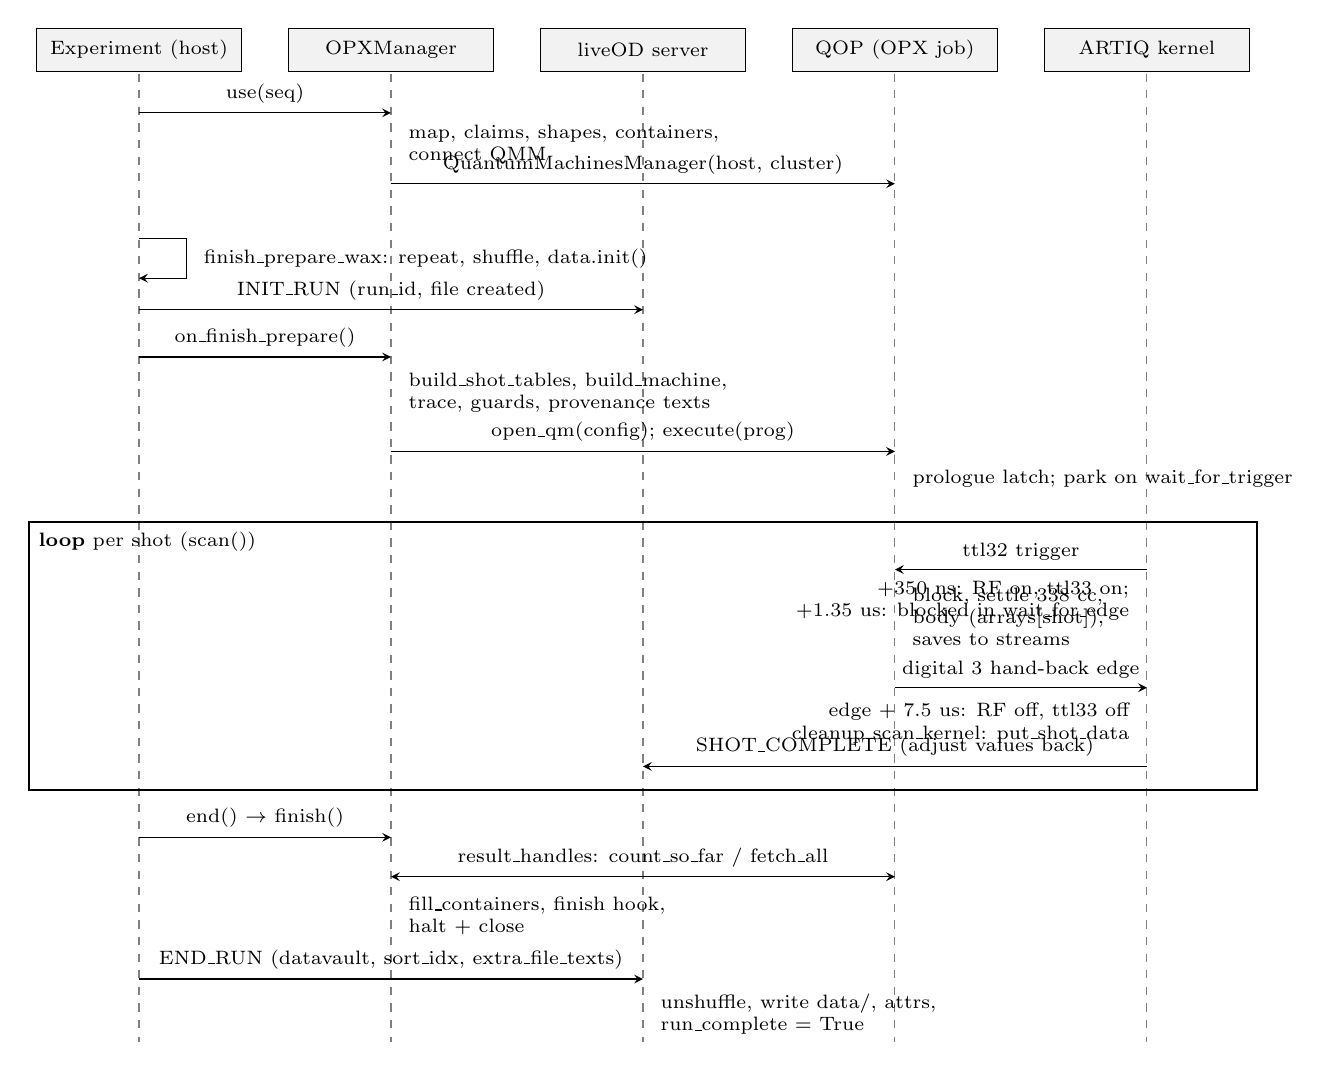
\begin{tikzpicture}[>=stealth, font=\scriptsize, x=1cm, y=1cm]
  % lifelines
  \foreach \x/\name in {0/Experiment (host), 3.2/OPXManager, 6.4/liveOD server, 9.6/QOP (OPX job), 12.8/ARTIQ kernel} {
    \node[draw, fill=gray!10, minimum width=2.6cm, minimum height=0.55cm] at (\x,0) {\name};
    \draw[dashed, gray] (\x,-0.3) -- (\x,-12.6);
  }
  % prepare
  \draw[->] (0,-0.8) -- (3.2,-0.8) node[midway, above] {use(seq)};
  \node[anchor=west, align=left] at (3.3,-1.2) {map, claims, shapes, containers,\\connect QMM};
  \draw[->] (3.2,-1.7) -- (9.6,-1.7) node[midway, above] {QuantumMachinesManager(host, cluster)};
  % finish_prepare
  \draw[->] (0,-2.4) -- (0.6,-2.4) -- (0.6,-2.9) -- (0,-2.9);
  \node[anchor=west] at (0.7,-2.65) {finish\_prepare\_wax: repeat, shuffle, data.init()};
  \draw[->] (0,-3.3) -- (6.4,-3.3) node[midway, above] {INIT\_RUN (run\_id, file created)};
  \draw[->] (0,-3.9) -- (3.2,-3.9) node[midway, above] {on\_finish\_prepare()};
  \node[anchor=west, align=left] at (3.3,-4.35) {build\_shot\_tables, build\_machine,\\trace, guards, provenance texts};
  \draw[->] (3.2,-5.1) -- (9.6,-5.1) node[midway, above] {open\_qm(config); execute(prog)};
  \node[anchor=west] at (9.7,-5.45) {prologue latch; park on wait\_for\_trigger};
  % run loop
  \draw[thick] (-1.4,-6.0) rectangle (14.2,-9.4);
  \node[anchor=north west] at (-1.4,-6.0) {\textbf{loop} per shot (scan())};
  \draw[->] (12.8,-6.6) -- (9.6,-6.6) node[midway, above] {ttl32 trigger};
  \node[anchor=east, align=right] at (12.7,-7.0) {+350 ns: RF on, ttl33 on;\\+1.35 us: blocked in wait\_for\_edge};
  \node[anchor=west, align=left] at (9.7,-7.2) {block, settle 338 cc,\\body (arrays[shot]),\\saves to streams};
  \draw[->] (9.6,-8.1) -- (12.8,-8.1) node[midway, above] {digital 3 hand-back edge};
  \node[anchor=east, align=right] at (12.7,-8.55) {edge + 7.5 us: RF off, ttl33 off\\cleanup\_scan\_kernel: put\_shot\_data};
  \draw[->] (12.8,-9.1) -- (6.4,-9.1) node[midway, above] {SHOT\_COMPLETE (adjust values back)};
  % end
  \draw[->] (0,-10.0) -- (3.2,-10.0) node[midway, above] {end() $\to$ finish()};
  \draw[<->] (3.2,-10.5) -- (9.6,-10.5) node[midway, above] {result\_handles: count\_so\_far / fetch\_all};
  \node[anchor=west, align=left] at (3.3,-11.0) {fill\_containers, finish hook,\\halt + close};
  \draw[->] (0,-11.8) -- (6.4,-11.8) node[midway, above] {END\_RUN (datavault, sort\_idx, extra\_file\_texts)};
  \node[anchor=west, align=left] at (6.5,-12.25) {unshuffle, write data/, attrs,\\run\_complete = True};
\end{tikzpicture}
\caption{Who talks to whom, in order. The host never touches the OPX during
the scan; the per-shot coupling is purely the two TTL wires between the
kernel and the job. Sources: \file{manager.py} (\code{use},
\code{on\_finish\_prepare}, \code{finish}); \file{wax/waxx-src/waxx/base/expt.py}
(\code{finish\_prepare\_wax}, \code{end\_wax}, \code{\_notify\_shot\_complete});
\file{k-exp/kexp/base/control.py} (the two handshake kernels).}
\label{fig:sequence}
\end{figure}

\subsection{Interactive use: \code{OPXBench}}

\code{OPXBench} stands in for a prepared experiment in a notebook: real
\code{ExptParams}, the real \code{dds\_frame} defaults, an \code{xvar}
interface, no ARTIQ, no liveOD, no run id.\footnote{\file{k-exp/kexp/control/opx/bench.py}.}
\code{bench.simulate(seq, shots=2)} runs \code{use(simulate=True)} +
\code{on\_finish\_prepare()} with \code{\_exit\_after\_simulate = False}, returns
the simulator job and opens the pulse viewer. Its \code{xvar} runs values in
the order given (no shuffle, no repeats), so shot $k$ of the simulation is
\code{values[k]}. It constructs \code{self.raman} as a real
\code{RamanBeamPair} exactly as \file{kexp/base/devices.py} does, so the
Raman transition split (\code{raman\_transition\_to\_ifs}) is the lab's; this
is how the feedback port was compiled and timed on the QOP simulator. Its
\code{compute\_new\_derived} is a no-op, so a sequence that reads an
experiment-local derived parameter raises \code{AttributeError} from
\code{ctx.p} on the bench.

\section{How xvars become OPX values}
\label{sec:xvars}

The central promise of the framework is: \emph{shot $k$ on ARTIQ and shot $k$
on the OPX use the same parameter values}, including repeats, shuffling and
derived parameters, without any per-shot host traffic. This section follows
one parameter from \code{self.xvar(...)} to the QUA array the OPX reads.

\subsection{Declaring an xvar}

\begin{lstlisting}[style=py]
self.xvar('t_raman_pulse', np.linspace(0., 50., 20) * 1.e-6)
self.p.N_repeats = 1
\end{lstlisting}

\code{Scanner.xvar(key, values)} appends an \code{xvar} record (\code{key},
\code{values}, \code{position} = declaration index, \code{counter} = 0) and
creates the attribute on \code{ExptParams} if it does not exist, holding the
first value as a scalar.\footnote{\file{wax/waxx-src/waxx/base/scanner.py},
\code{xvar} (lines 103--119) and \code{new\_param\_check}.} Two xvars declared
$\to$ a 2-D grid, the \emph{last declared} innermost.

\subsection{\code{finish\_prepare}: repeats, then shuffle}
\label{sec:xvars:shuffle}

\code{Scanner.init\_xvars}\footnote{\file{scanner.py} lines 562--591.} runs,
in this order:

\begin{enumerate}[nosep]
  \item \code{plug\_in\_xvars}: \code{params.<key> = values[0]} so the kernel
    compiles against the scalar's type. This is the value every
    \emph{config-time} read sees (section~\ref{sec:program:config}).
  \item \code{repeat\_xvars}: \code{xvar.values = np.repeat(values,
    N\_repeats[position])}. With an integer \code{N\_repeats} only position 0
    -- the \textbf{outermost} (first-declared) axis -- is repeated; each value
    appears $N$ times \emph{consecutively}: $[a, b] \to [a, a, b, b]$.
    \code{params.N\_repeats} collapses back to the scalar. Repeats are not a
    separate axis.\footnote{\file{wax/waxa-src/waxa/base/dealer.py},
    \code{repeat\_xvars}, lines 36--75.}
  \item \code{shuffle\_xvars}: per axis, sort the values, draw one permutation
    of \code{arange(len)}, and \code{values.take(perm)}. Any later xvar of the
    same length \emph{reuses the same permutation}. The distinct lengths and
    their permutations are recorded as \code{sort\_N} / \code{sort\_idx} for the
    end-of-run unshuffle.\footnote{\file{dealer.py}, \code{shuffle\_xvars},
    lines 77--126. Note the equal-length rule at lines 105--107: a 2-xvar scan
    with equal lengths is \emph{correlated} in its shuffle.}
  \item \code{get\_N\_img}, \code{compute\_derived}, \code{compute\_new\_derived}
    at the first scheduled values; \code{xvardims = [len(values) ...]},
    repeats included; \code{generate\_assignment\_kernels}.
\end{enumerate}

\statusbox{Which shuffle scheme this is.}{The per-axis scheme above
(\code{Dealer.shuffle\_xvars} + \code{sort\_idx}/\code{sort\_N}) is what the
tree contains. The wiki page \emph{Scan loop and parameter scanning} and the
memory note \emph{random-scan-order} describe a full-grid random order with a
\code{run\_info/shot\_order} dataset; that work lives in a git stash on the
branch \code{jep/random-scan-order-new} and is \textbf{not} in this checkout
(\code{wax} is on \code{main}; \code{grep shot\_order} over \code{wax/} finds
nothing). Everything in this document assumes the per-axis scheme. If the
stash lands, \code{build\_shot\_tables} must sweep \code{shot\_order} instead
of \code{np.ndindex}, and \code{fill\_containers} must scatter instead of
reshape.}

\subsection{The scan loop on ARTIQ: reassign, never index}
\label{sec:xvars:scanloop}

\code{Scanner.scan()} is a compiled \code{@kernel} \code{while} loop. Per
iteration:\footnote{\file{scanner.py} lines 282--378.}

\begin{lstlisting}[style=py]
aborted_bool = self._check_for_abort_signal()     # RPC
self.update_params_from_xvars()                   # RPC: host params <- xvar values, adjust, derived
self.write_host_params_to_kernel()                # kernel: one RPC fetch + writer per param
self.core.break_realtime()
self.init_scan_kernel()
try:
    self.scan_kernel()                            # the experiment
except RTIOUnderflow / TriggerTimeout / RTIOOverflow:
    aborted_bool = True                           # cleanup still runs
self.cleanup_scan_kernel()                        # put_shot_data, SHOT_COMPLETE
delay(self.params.t_recover)
scanning = self.step_scan()                       # RPC: odometer on the host counters
self.update_scan_xvar_counters()                  # kernel mirrors the counters
\end{lstlisting}

\code{update\_params\_from\_xvars} is the host side:

\begin{lstlisting}[style=py]
for xvar in self.scan_xvars:
    vars(self.params)[xvar.key] = xvar.values[xvar.counter]
self.apply_pending_adjust_values()
self.params.compute_derived()
self.compute_new_derived()
\end{lstlisting}

So on the host the scanned attribute \textbf{is a scalar that is reassigned
every shot} from the repeated, shuffled list. The kernel copy is then
refreshed by \code{write\_host\_params\_to\_kernel}: for each int32/int64/float/
array attribute of \code{ExptParams}, one RPC fetch and one pre-generated
writer kernel whose source is literally \code{self.params.<key> = value}
(\code{generate\_assignment\_kernels}, \file{scanner.py} lines 490--514). The
kernel never indexes \code{xvar.values}; the counters on the kernel are only
a mirror for \code{put\_shot\_data}. \code{step\_scan} increments the host
counters like an odometer starting from the last-declared xvar (C order).

\subsection{\code{build\_shot\_tables}: the same sweep, on a copy}
\label{sec:xvars:tables}

The OPX cannot run \code{update\_params\_from\_xvars}. Instead, at
\code{on\_finish\_prepare}, \code{build\_shot\_tables(expt)} replays the
sweep once on a deep copy of \code{ExptParams}:\footnote{\file{k-exp/kexp/control/opx/params\_bridge.py},
\code{build\_shot\_tables} (lines 315--344) and \code{working\_params}.}

\begin{lstlisting}[style=py]
with working_params(expt) as work:            # deep copy; expt.params/expt.p swapped for the block
    for idx in np.ndindex(*xvardims):         # C order = last xvar innermost = step_scan's order
        for xvar, i in zip(expt.scan_xvars, idx):
            vars(work)[xvar.key] = xvar.values[i]
        work.compute_derived()
        expt.compute_new_derived()            # runs on the copy (expt.params is swapped)
        # snapshot every scalar numeric attribute -> columns[key][flat]
\end{lstlisting}

The result, \code{ShotTables}, holds \code{columns[key]}: a float array of
length \code{n\_shots} in \textbf{execution order} for every scalar numeric
attribute (bool, int, float, numpy scalars). Arrays and strings are not
shipped; a vector-valued xvar is therefore invisible to \code{ctx.p} and
raises \code{AttributeError} there. \code{tables.accessed} records which
columns the sequence read. Cost, measured on the 298-attribute
\code{ExptParams}: one deep copy (0.11\,ms) and 0.056\,ms per shot -- about
0.6\,s for a 10\,000-shot scan.

\subsection{\code{ParamRef}: a column that refuses to be a number}
\label{sec:xvars:paramref}

\code{ctx.p} is a \code{ParamsProxy}; \code{ctx.p.t\_raman\_pulse} returns a
\code{ParamRef(key, column, tables)} and marks the key accessed. A
\code{ParamRef} supports ordinary arithmetic and numpy ufuncs \emph{column-wise
on the host}: \code{ctx.p.t\_raman\_pi\_pulse / 2} is a new \code{ParamRef}
labelled \code{(t\_raman\_pi\_pulse / 2)} whose column is computed shot by
shot. What it cannot do is collapse to one Python number:
\code{float()}, \code{int()}, \code{bool()} -- and with them \code{if},
\code{max()}, \code{in}, \code{np.sum()} -- raise a \code{TypeError} with a
hint.\footnote{\file{params\_bridge.py}, class \code{ParamRef}, lines
102--251.} The reason is the trace-once model of section~\ref{sec:program}:
the body runs \emph{once} on the host to emit QUA; a Python \code{if} on a
scanned value would pick one shot's branch and bake it into every shot,
silently mislabelling the scan.

\code{ctx.const(x)} is the explicit escape: it returns a float for a number
or for a \code{ParamRef} whose column is the same on every shot (a loop
count, a toggle), and refuses one that varies:

\begin{lstlisting}[style=txt]
[opx] sequence 'bayesian_feedback': ctx.const('N_pulses') but it varies per shot
(17 .. 20) -- it is scanned, or derived from a scanned parameter. ctx.const gives
one number the whole program is built with; a per-shot value must reach the OPX
through a ctx method (or ctx.cc/ctx.hz/ctx.f).
\end{lstlisting}

\subsection{Materialisation: baked constant or QUA array indexed by the shot counter}
\label{sec:xvars:resolve}

Every context macro ends in \code{OPXShotContext.\_resolve(x, transform,
tag, qua\_dtype, what)}:\footnote{\file{k-exp/kexp/control/opx/context.py},
\code{\_resolve}, lines 119--152.}

\begin{lstlisting}[style=py]
col = np.atleast_1d(np.asarray(transform(raw)))   # SI -> cc / integer Hz / fixed, per shot
# finite check; int32 range check (|v| < 2^31) or fixed range check ([-8, 8))
if np.all(col == col[0]):
    v = col[0]
    return int(v) if qua_dtype is int else float(v)        # baked constant
values = [int(v) for v in col]  (or floats)
cache_key = (tag, tuple(values))                            # keyed by value
if cache_key not in self._qua_arrays:
    self._qua_arrays[cache_key] = qua.declare(int or qua.fixed, value=values)
return self._qua_arrays[cache_key][self._shot]              # QUA array cell, indexed by the shot counter
\end{lstlisting}

A constant and a per-shot column take the same path (transform, then range
checks), so whether a value is valid never depends on whether it happens to
be scanned this run. A per-shot column becomes one \code{qua.declare(...,
value=[...])} array of length \code{n\_shots} and the program reads
\code{arr[shot]}, where \code{shot} is the loop variable of the builder's
\code{for\_(shot, 0, shot < n\_shots, shot + 1)}. Two expressions with
identical columns share one array. \code{ctx.cc()}, \code{ctx.hz()} and
\code{ctx.f()} also accept a QUA expression and return it unchanged
(\code{is\_qua\_expr}: taken to be clock cycles / integer Hz / fixed already,
no host checks, no value column in the op log), which is how a real-time loop
feeds a value the OPX computed into a macro.

\subsection{Derived parameters}

Because the sweep runs the real \code{compute\_derived()} and the
experiment's \code{compute\_new\_derived()} per shot, a parameter derived from
an xvar varies per shot on the OPX \emph{by construction}, not by a parallel
reimplementation. The offline check below includes \code{t\_double = 2 t\_a}
defined in \code{compute\_new\_derived}. The caveat: \code{compute\_new\_derived}
is called on the copy, but anything it reads that is \emph{not} on
\code{ExptParams} (an attribute of the experiment, a random draw) is whatever
it was at \code{finish\_prepare} (section~\ref{sec:midloop:holes}).

\subsection{The offline order-equivalence check}
\label{sec:xvars:check}

The phase-1 audit drove the real \code{Scanner}, \code{Dealer},
\code{DataVault}, \code{build\_shot\_tables} and \code{fill\_containers} with no
core device for a 3\,$\times$\,2 scan, \code{N\_repeats = 2}, default per-axis
shuffle, plus a derived parameter. Its output, verbatim:\footnote{\code{scratchpad/phase1/check\_scan\_order.py},
run with the workspace venv on 2026-09-24. The \code{np.float64(...)} wrappers
are numpy~2's scalar repr.}

\begin{lstlisting}[style=txt]
xvardims after repeats: [6, 2]  N_repeats -> 2
  xvar 't_a' (position 0) execution values: [3.e-06 1.e-06 2.e-06 2.e-06 1.e-06 3.e-06]
  xvar 'i_b' (position 1) execution values: [20. 10.]
sort_N: [6, 2]  sort_idx: [[np.int64(4), np.int64(0), np.int64(3), np.int64(2), np.int64(1), np.int64(5)], [np.int64(1), np.int64(0)]]

12 shots.  shot | ARTIQ (t_a, i_b, t_double) counters | OPX tables (t_a, i_b, t_double) ndindex
   0 | (np.float64(3e-06), np.float64(20.0), np.float64(6e-06)) (0, 0) | (np.float64(3e-06), np.float64(20.0), np.float64(6e-06)) (0, 0)
   1 | (np.float64(3e-06), np.float64(10.0), np.float64(6e-06)) (0, 1) | (np.float64(3e-06), np.float64(10.0), np.float64(6e-06)) (0, 1)
   2 | (np.float64(1e-06), np.float64(20.0), np.float64(2e-06)) (1, 0) | (np.float64(1e-06), np.float64(20.0), np.float64(2e-06)) (1, 0)
   3 | (np.float64(1e-06), np.float64(10.0), np.float64(2e-06)) (1, 1) | (np.float64(1e-06), np.float64(10.0), np.float64(2e-06)) (1, 1)
   4 | (np.float64(2e-06), np.float64(20.0), np.float64(4e-06)) (2, 0) | (np.float64(2e-06), np.float64(20.0), np.float64(4e-06)) (2, 0)
   5 | (np.float64(2e-06), np.float64(10.0), np.float64(4e-06)) (2, 1) | (np.float64(2e-06), np.float64(10.0), np.float64(4e-06)) (2, 1)
   6 | (np.float64(2e-06), np.float64(20.0), np.float64(4e-06)) (3, 0) | (np.float64(2e-06), np.float64(20.0), np.float64(4e-06)) (3, 0)
   7 | (np.float64(2e-06), np.float64(10.0), np.float64(4e-06)) (3, 1) | (np.float64(2e-06), np.float64(10.0), np.float64(4e-06)) (3, 1)
   8 | (np.float64(1e-06), np.float64(20.0), np.float64(2e-06)) (4, 0) | (np.float64(1e-06), np.float64(20.0), np.float64(2e-06)) (4, 0)
   9 | (np.float64(1e-06), np.float64(10.0), np.float64(2e-06)) (4, 1) | (np.float64(1e-06), np.float64(10.0), np.float64(2e-06)) (4, 1)
  10 | (np.float64(3e-06), np.float64(20.0), np.float64(6e-06)) (5, 0) | (np.float64(3e-06), np.float64(20.0), np.float64(6e-06)) (5, 0)
  11 | (np.float64(3e-06), np.float64(10.0), np.float64(6e-06)) (5, 1) | (np.float64(3e-06), np.float64(10.0), np.float64(6e-06)) (5, 1)

values identical shot-for-shot: True
counter tuples == np.ndindex tuples: True
tables.n_shots == shots the loop ran: True
[opx] NOTE: 'sig' stored as raw integration units (no integration window length known).
[opx] data complete: 12/12 shots.
kernel-path _run_data shape: (6, 2)  fill_containers _run_data shape: (6, 2)
kernel-path == fill_containers, cell for cell: True
valid mask: [[1 1]
 [1 1]
 [1 1]
 [1 1]
 [1 1]
 [1 1]]
unshuffled arrays equal: True
every unshuffled cell holds a shot taken at that (t_a, i_b): True

RESULT: ORDER EQUIVALENT
\end{lstlisting}

Read-offs: the repeat is folded into the outer axis as consecutive
duplicates \emph{before} shuffling, so after the per-axis shuffle repeats of
the same value are no longer adjacent ($3, 1, 2, 2, 1, 3$); the inner xvar
changes every shot; the derived column follows the xvar; the DataContainer
cell index equals the \code{ndindex} tuple; and the flat execution-order
stream that \code{fill\_containers} writes lands in the same cells as the
kernel's per-shot writes, so the single end-of-run unshuffle treats both
identically.

What the check does \emph{not} cover, because no code covers it: the ARTIQ
shot index and the OPX \code{shot} counter are tied only by one
\code{wait\_for\_trigger} per \code{scan\_kernel}. A \code{scan\_kernel} that
skips \code{handoff\_to\_quantum\_machines} on some shots, or triggers twice,
desynchronises the counters for the rest of the run. The shot-index echo of
section~\ref{sec:data:echo} detects this after the fact; nothing prevents
it. (The warm-up shots of \code{Base.pre\_scan} do not hand off and are safe.)

\subsection{Shot arrays and host data}
\label{sec:xvars:shotarrays}

A per-shot \emph{scalar} is a column; some sequences need a per-shot
\emph{vector} -- the feedback loop draws $N$ pulse durations per shot. Two
context calls exist for that:\footnote{\file{context.py}, \code{ShotArray},
\code{OPXShotContext.shot\_array}, \code{host\_data}.}

\begin{itemize}[nosep]
  \item \code{ctx.shot\_array(key, values, dtype=float)}: \code{values} is an
    array of shape \code{(n\_shots,)} or \code{(n\_shots, M)} in execution
    order, validated finite and in range (integral and int32 for
    \code{dtype=int}, fixed $[-8, 8)$ for float); it becomes \emph{one} flat
    QUA array and \code{ShotArray.at(i)} returns \code{qua\_array[ctx.shot * M
    + i]} (\code{i} a Python int, bounds-checked, or a QUA int expression, not
    checked -- QUA does no bounds checking either). QUA arrays are 1-D only,
    which is why the 2-D table is flattened. Declaring a key twice is
    refused; the shapes are recorded in \code{opx\_shot\_tables}.
  \item \code{ctx.host\_data(key, values)}: \code{values} of shape
    \code{(n\_shots, *shape)} are written straight into a container declared
    in the sequence's \code{host\_data=\{key: shape\}} at \code{finish()}, in
    execution order, never volts-converted. This is how the run file records
    exactly what the OPX was given (section~\ref{sec:feedback:data}).
\end{itemize}

The spec's decision D6: per-shot arrays are pre-drawn on the host at trace
time and shipped as baked arrays; QUA input streams (host pushes per shot)
are \emph{not} used in v1 because the simulator cannot run them. The hook
for them is the top of the shot loop, before \code{wait\_for\_trigger}.

\section{How the QUA program is constructed}
\label{sec:program}

\subsection{Trace once, execute per shot}

A sequence is a plain Python function of one argument, the context
\code{ctx}, decorated with \code{@opx\_sequence}:\footnote{\file{k-exp/kexp/experiments/opx\_sequences/rabi.py};
\file{k-exp/kexp/control/opx/sequence.py}.}

\begin{lstlisting}[style=py]
@opx_sequence('rabi_raman_pulse', claims=('raman',))
def rabi_raman_pulse(ctx: KexpShotContext):
    ctx.raman_pulse(ctx.p.t_raman_pulse)
\end{lstlisting}

The function body is executed \textbf{exactly once}, on the host, inside
\code{with qua.program()}. Every \code{ctx} call emits QUA statements into
that program. The OPX then executes the program's shot loop \code{n\_shots}
times. This is what ``trace-time'' means throughout this document: the
sequence author writes what looks like one shot; the builder wraps it in the
loop and the context turns every parameter into either a constant or an
\code{arr[shot]} lookup (section~\ref{sec:xvars:resolve}). Consequently a
Python \code{for i in range(int(ctx.const(ctx.p.N)))} unrolls $N$ copies of
its body into the program, while \code{with ctx.for\_range(n) as i:} emits a
QUA loop (section~\ref{sec:tutorial}).

The decorator records the sequence's \code{claims} (which roles it may touch:
\code{'raman'}, \code{'imaging'}), its \code{measurements} (which data keys it
saves, and its per-shot shape), its \code{host\_data} keys and an optional
\code{finish} hook. Ops on an unclaimed role, saves
to an undeclared key, and a save count that disagrees with the declaration
are trace-time errors.

\subsection{The emitted statement skeleton}
\label{sec:program:skeleton}

What \code{OPXProgramBuilder.trace()} emits after the rebuild, with the real
numbers for the default parameters:\footnote{\file{k-exp/kexp/control/opx/builder.py},
\code{trace}; hand-back in \file{context.py}, \code{handback\_to\_artiq}.
Settle and overlap from \file{k-exp/kexp/config/expt\_params.py} lines
438--439 and 455.}

\begin{lstlisting}[style=qua]
with program():
    shot = declare(int)
    echo = declare_output_stream()                            # the shot-index echo stream
    # one declare(int|fixed, value=[...N_shots...]) per distinct per-shot column (at first use)
    # one declare_output_stream() (+ a fixed variable for measure keys) per data key (at first use)

    # ---- prologue, once per run ----
    play('cw' * amp(sqrt(f)), 'raman_80')                     # f = fraction_power_raman (ARTIQ's);
    play('cw' * amp(sqrt(f)), 'raman_150')                    #   1000 ns sticky latch; tone holds all run

    with for_(shot, 0, shot < N_shots, shot + 1):             # implicit align at loop entry
        [update_frequency('raman_150', ifs150[shot]); update_frequency('raman_80', ifs80[shot])]
                                                              #   only if frequency_raman_transition varies
        wait_for_trigger('raman_switch')                      # park until ARTIQ's ttl32 edge
        save(shot, echo)                                      # counter echo -> 'opx_shot_index'
        align()                                               # A1: everyone else catches up
        play('block', 'raman_switch'); play('block', 'imaging_switch')   # 16 ns markers, sticky-held HIGH
        wait(338, 'raman_switch', 'imaging_switch')           # settle = artiq_side + opx_side = 1.35 us, both guarded switches
        align()                                               # A3: body starts on every element together

        <sequence body>                                       # e.g. play('pass','raman_switch',duration=d[shot]); play('block','raman_switch')

        align()                                               # A4: trigger follows the body's last statement
        play('trigger', 'artiq_handback')                     # 200 ns rising edge -> ttl41
        wait(3750, 'raman_switch', 'imaging_switch')          # overlap = 15 us; ARTIQ takes RF back at 7.5 us
        play('pass', 'raman_switch'); play('pass', 'imaging_switch')     # blocks released
        [align(); update_frequency(... run transition ...)]   # A5, only if the body moved a drive

    # ---- epilogue, once per run ----
    ramp_to_zero('raman_80'); ramp_to_zero('raman_150')       # 100 ns ramp
    align()

    with stream_processing():
        <stream>.buffer(n).save_all(key)                      # per key; 2-D (n1, n2): .buffer(n2).buffer(n1)
        echo.save_all('opx_shot_index')                       # one int per shot
\end{lstlisting}

Before the rebuild the framing had two more global aligns (one between the
block plays and the settle wait, one inside every \code{wait\_s}), waited the
settle on the sync element only, and read the settle from a parameter that no
longer exists (\code{t\_opx\_handoff\_settle}; section~\ref{sec:handoff}).
\code{settle\_cc = s\_to\_cc(1.35e-6) = 338}: $1350/4 = 337.5$ rounds to 338,
i.e.\ 1352\nsu, a 0.15\,\% rounding, below the 1\,\% warning threshold.

\subsubsection{Why each align exists}

\code{align()} with no arguments makes every element used in the program wait
for all the others to finish their current statement. A deterministic align
(no QUA-variable dependence upstream) compiles to a plain wait with no gap; one
that follows a trigger, a variable-duration play or a branch costs ``a few
cycles'' of hardware synchronisation (QM publishes no number).

\begin{table}[htbp]
\centering
\small
\begin{tabular}{@{}lll@{}}
\toprule
align & needed? & why \\
\midrule
A1 after \code{wait\_for\_trigger} & yes & only \code{raman\_switch} waited; \code{imaging\_switch}, the drives and \code{apd} must not run ahead \\
(old A2 after the block plays) & no, removed & both switches were aligned by A1; the settle wait is now issued on both switches \\
A3 after the settle wait & yes & brings \code{apd}, \code{raman\_80/150} to the body start; a body \code{set\_transition} relies on it \\
inside \code{measure} & element-scoped & \code{align(switch, apd)} so the ADC window starts with the exposure \\
A4 before the hand-back & yes & the trigger must follow the body's last play/measure on every element \\
A5 after the release & only if a drive was re-pointed & a following \code{update\_frequency} runs at the drive element's own cursor, which otherwise sits at the last align \\
\bottomrule
\end{tabular}
\caption{Aligns in the per-shot framing. A body may add its own:
\code{ctx.align(*names)}; \code{ctx.wait\_s} (one global align, then a
\code{wait} on every element the map names); \code{ctx.measure} (one
element-scoped align of switch and detector); \code{phase\_reset=True} (one
align of the two drives with the switch, where the resets land).}
\label{tab:aligns}
\end{table}

\subsection{The element / core model}

Each QUA \emph{element} is a named logical channel bound to ports and running
on its own core; statements on different elements execute in parallel and are
ordered only by aligns, waits on named elements, and the implicit aligns at
loop/branch entry. Our program uses seven elements (well inside the 18-core
limit):

\begin{table}[htbp]
\centering
\small
\begin{tabular}{@{}llll@{}}
\toprule
element & ports & sticky & ops \\
\midrule
\code{raman\_80} & analog out 1 & analog, 100\nsu\ ramp & \code{cw} (1000\nsu\ latch, constant waveform = dds default 0.337\,V = power fraction 1, played at \code{amp(}$\sqrt{f}$\code{)}) \\
\code{raman\_150} & analog out 2 & analog, 100\nsu\ ramp & \code{cw} (0.324\,V) \\
\code{raman\_switch} & digital 1 & analog+digital, 16\nsu & \code{block} $[(1,0)]$, \code{pass} $[(0,0)]$, both 16\nsu\ long \\
\code{imaging\_switch} & digital 2 & analog+digital, 16\nsu & \code{block}, \code{pass} \\
\code{artiq\_handback} & digital 3 & none & \code{trigger} $[(1,0)]$, 200\nsu \\
\code{apd} & analog in 1, marker digital 4 & none & \code{acquire}: measurement pulse of \code{t\_imaging\_pulse\_apd\_abs}, \code{time\_of\_flight} 200\nsu, weights \code{integration\_window} (\code{t\_opx\_integration\_start/len}) and \code{full\_pulse} \\
\bottomrule
\end{tabular}
\caption{Elements of the K-machine OPX config.
\file{k-exp/kexp/control/opx/opx\_config.py}, \code{build\_machine}: a
\code{components.Machine} whose \code{generate\_config()} emits this
\code{elements} block; the pulse, waveform, marker and weight entries behind
it are named \code{<element>.<label>.pulse|wf|dm} and
\code{<element>.<label>.<weight>.iw} (the golden test compares the
\code{elements} block with the previous hand-written config). Amplitudes from
\file{kexp/config/dds\_id.py} lines 84--86 and 110--112; they are the
$f = 1$ amplitudes, and the builder's latch scales them by $\sqrt{f}$ with
$f$ = \code{fraction\_power\_raman} (\code{ChannelSpec.power\_fraction\_param}),
the same factor \code{RamanBeamPair.set} applies to the DDSs. $f$ must be
constant for the run (refused as an xvar or \code{adjust()} key when the
sequence claims \code{raman}).}
\label{tab:elements}
\end{table}

The sync element is \code{raman\_switch}: it alone executes
\code{wait\_for\_trigger}; A1 brings the rest to it. The sticky drives
\code{raman\_80/150} and \code{apd} are only ever moved by aligns and by
their own few statements (latch, \code{update\_frequency},
\code{reset\_if\_phase}, \code{measure}), so their element clocks sit at the
last align -- the reason A5 exists.

\subsection{Units: SI in, clock cycles / integer Hz out}
\label{sec:program:units}

Everything a sequence writes is SI. Conversion is host-side, per shot, in
\file{units.py}:\footnote{\file{k-exp/kexp/control/opx/units.py}.}

\begin{itemize}[nosep]
  \item \code{s\_to\_cc(t)}: seconds $\to$ integer clock cycles,
    \code{np.rint(ns / 4)}. Prints an unconditional warning when the 4\nsu\
    grid moves any value by more than 1\,\% (\code{GRID\_WARN\_REL}) of what
    was requested; \textbf{raises} when a nonzero duration rounds below the
    16\nsu\ minimum (\code{MIN\_PULSE\_CC = 4}) -- silently stretching a
    pulse would misreport what the machine did. A zero is allowed (the
    macros then play nothing or guard with \code{if\_}).
  \item \code{s\_to\_ns(t)}: for config pulse lengths (integer ns).
  \item \code{hz\_to\_int(f)}: integer Hz for \code{update\_frequency} and
    config IFs (1\,Hz resolution; the AD9910 FTW quantum is 0.23\,Hz).
  \item \code{ctx.f(x)}: a plain float that must fit QUA fixed $[-8, 8)$.
\end{itemize}

The context then range-checks: \code{\_check\_finite} (NaN/inf name the
offending shots), \code{\_check\_int32} ($|v| < 2^{31}$: ``durations of 8.6\,s
or more, frequencies of 2.1\,GHz or more. A seconds-vs-microseconds slip?''),
\code{\_check\_fixed}. Note the difference from the customer scripts, which
\emph{floor} to the grid (\code{//4}) and add a 4\nsu\ ramp to every exposure;
the builder's \code{pass} play has no such offset.

\subsection{Config-time versus shot-time parameters, and the guard}
\label{sec:program:config}

Some numbers are compiled into the QUA \emph{config} once per run and cannot
change per shot: the Raman drive IFs and amplitudes, the APD acquire pulse
length, the integration weights, and the two handshake windows. Everything
else -- pulse durations, detunings, phases -- is shot-time and scans freely.

\paragraph{The Raman IFs have a shot-time route built in.} The config IFs are
computed at the \emph{first executed shot's} \code{frequency\_raman\_transition}
(\code{raman\_config\_transition}, which reads \code{tables.column(key)[0]}) by
\code{expt.raman.ao\_frequencies}, the same \code{state\_splitting\_to\_ao\_frequency}
split \code{RamanBeamPair.set} runs in the kernel. For the default transition
$\Delta = 119.4639$\,MHz: $f_{150} = 143.303446$\,MHz, $f_{80} =
83.571496$\,MHz, with $2(f_{150} - f_{80}) = \Delta$ (double pass). When the
transition varies per shot the builder re-points both drives at the top of
every shot (\code{update\_frequency} with \code{ifs[shot]}); a body that moves
a drive (\code{ctx.set\_transition} for a Ramsey detuning) is restored after
the hand-back.\footnote{\file{opx\_config.py}, \code{raman\_transition\_to\_ifs},
\code{raman\_config\_transition}; \file{wax/waxx-src/waxx/control/raman\_beams.py},
\code{ao\_frequencies}.}

\paragraph{The others are refused as xvars and as adjust keys (D2).} At the
moment \code{build\_machine} reads them, a scanned key holds
\code{values[0]} from \code{plug\_in\_xvars} -- the smallest declared value --
so the acquire window would be baked at that value while ARTIQ scans it.
\file{opx\_config.py} defines\footnote{\file{opx\_config.py},
\code{CONFIG\_TIME\_PARAMS} and \code{config\_time\_params(expt, tables)};
carried on \code{ChannelMap.config\_time\_params};
\code{check\_config\_time\_xvars} in \file{manager.py}.}
\begin{lstlisting}[style=py]
CONFIG_TIME_PARAMS = ('t_imaging_pulse_apd_abs', 't_opx_integration_start',
                      't_opx_integration_len', 't_opx_handoff_artiq_side',
                      't_opx_handoff_opx_side', 't_opx_handback_overlap')
\end{lstlisting}
(\code{frequency\_raman\_transition} is deliberately \emph{not} in the list:
it is compiled at the first executed shot's value but re-pointed per shot,
and it is still recorded as accessed so it cannot be live-adjusted). Three
checks enforce the list: \code{check\_config\_time\_xvars} refuses any of them
in \code{expt.xvarnames}, at \code{use()} (before a run id exists) and again
at \code{on\_finish\_prepare}; \code{config\_time\_params(expt, tables)},
called from \code{build\_machine}, adds every key to \code{tables.accessed}
(so \code{check\_live\_adjust\_conflicts} covers them) and raises if a key's
column varies per shot -- which also catches a config-time parameter
\emph{derived} from a scanned one; and the manager adds the keys to
\code{accessed} itself. Scanning the acquire length therefore needs a
shot-time route (\code{ctx.measure(t\_expose=...)} for the exposure; the ADC
window itself is fixed per run).

\paragraph{Amplitudes.} The OPX drives the AOs at the dds-frame defaults used
directly as waveform sample volts (0.337\,V / 0.324\,V, guarded against the
0.499\,V full scale), whereas the ARTIQ path programs
$\sqrt{\code{fraction\_power\_raman}}\times$default $= 0.548\times$default. The
Rabi rate, hence \code{t\_raman\_pi\_pulse} and every $\Omega$-scaled quantity
in section~\ref{sec:feedback}, depends on this and must be re-measured on the
OPX drive (M2).

\subsection{The op log and the pulse viewer}

Every statement the context or builder emits is also appended to an
\code{OpLog} as an \code{OpRecord}: kind, element, op, phase (prologue /
handshake / body / epilogue), the macro that produced it, the parameter
expression and its per-shot values, the requested duration per shot, the
shots on which it executes (a per-shot \code{if\_} guard), and the source line
chain in the sequence file.\footnote{\file{k-exp/kexp/control/opx/trace\_log.py}.}
Nothing here changes the program; the pulse viewer (\code{waxx.util.seqview}
via \code{kexp.control.opx.viewer}) matches the log against the simulator's
waveform report so every simulated pulse points back at the Python line and
the generated QUA line that made it. This is a provenance feature QUAM does
not have (section~\ref{sec:quam}).

\section{The handoff}
\label{sec:handoff}

One OPX window per shot: ARTIQ triggers, turns its RF on for the OPX to gate,
and blocks until the OPX says it is done; then ARTIQ takes the RF back while
the OPX still holds the blocks. Four numbers govern it, all in
\code{ExptParams}:\footnote{\file{k-exp/kexp/config/expt\_params.py} lines
438--439, 455; \code{T\_OPX\_TRIGGER\_PULSE}/\code{T\_OPX\_HANDBACK\_TIMEOUT} in
\file{k-exp/kexp/base/control.py} lines 33--34.}

\begin{center}\small
\begin{tabular}{@{}llp{8.6cm}@{}}
\toprule
parameter & value & meaning \\
\midrule
\code{t\_opx\_handoff\_artiq\_side} & 350\nsu & trigger $\to$ ARTIQ RF on. \textbf{Unmeasured assumption} (M1): the OPX must have seen the trigger and raised its blocks by then \\
\code{t\_opx\_handoff\_opx\_side} & 1\us & RF-switch turn-off (MOSFET inverter) + ARTIQ DDS RF-switch rise time; ARTIQ returns to the caller at the sum, 1.35\us \\
\code{t\_opx\_handback\_overlap} & 15\us & OPX holds the blocks this long after its hand-back edge; ARTIQ takes the RF back at \emph{half} of it (7.5\us) \\
\code{T\_OPX\_TRIGGER\_PULSE} & 1\us & width of the ttl32 trigger pulse (cursor is rewound, so 0 timeline cost) \\
\code{T\_OPX\_HANDBACK\_TIMEOUT} & 2\,s & no edge by then $\to$ \code{TriggerTimeout} \\
\bottomrule
\end{tabular}
\end{center}

Decision D1 of the spec: the OPX settle wait is the \emph{sum}
\code{artiq\_side + opx\_side}, carried on the channel map as one field
\code{t\_handoff\_settle\_s} that \code{kexp\_channel\_map} fills with that
sum (\code{settle\_s = artiq\_side + opx\_side}, also recorded in the
machine's \code{extra}). Before the rebuild the map read a parameter
(\code{t\_opx\_handoff\_settle}) that commit \code{b77c728c} had replaced,
so every \code{self.opx.use(...)} died with \code{AttributeError} in
\code{prepare()}; the test fixtures fabricated the old name and passed.

\subsection{Timing diagram (a): as coded after the rebuild}
\label{sec:handoff:diag_a}

\begin{figure}[htbp]
\centering
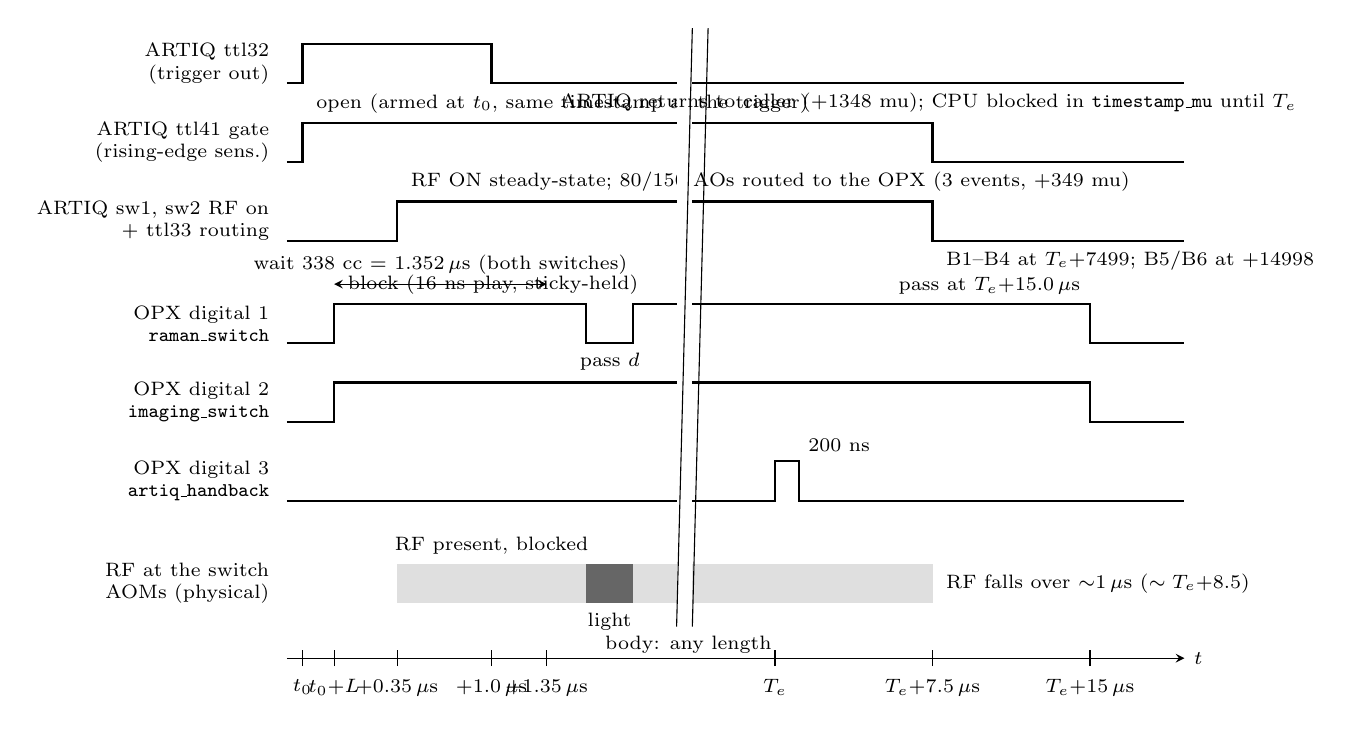
\begin{tikzpicture}[>=stealth, font=\scriptsize, x=1cm, y=1cm]
  % lane labels
  \node[anchor=east, align=right] at (0.7,6.25) {ARTIQ ttl32\\(trigger out)};
  \node[anchor=east, align=right] at (0.7,5.25) {ARTIQ ttl41 gate\\(rising-edge sens.)};
  \node[anchor=east, align=right] at (0.7,4.25) {ARTIQ sw1, sw2 RF on\\+ ttl33 routing};
  \node[anchor=east, align=right] at (0.7,2.95) {OPX digital 1\\\code{raman\_switch}};
  \node[anchor=east, align=right] at (0.7,1.95) {OPX digital 2\\\code{imaging\_switch}};
  \node[anchor=east, align=right] at (0.7,0.95) {OPX digital 3\\\code{artiq\_handback}};
  \node[anchor=east, align=right] at (0.7,-0.35) {RF at the switch\\AOMs (physical)};
  % ttl32: low 0.8-1.0, high 1.0-3.4, low after
  \draw[thick] (0.8,6.0) -- (1.0,6.0) -- (1.0,6.5) -- (3.4,6.5) -- (3.4,6.0) -- (12.2,6.0);
  % gate: open 1.0 -> 9.0
  \draw[thick] (0.8,5.0) -- (1.0,5.0) -- (1.0,5.5) -- (9.0,5.5) -- (9.0,5.0) -- (12.2,5.0);
  \node[anchor=south west] at (1.05,5.5) {open (armed at $t_0$, same timestamp as the trigger)};
  % sw/ttl33: high 2.2 -> 9.0
  \draw[thick] (0.8,4.0) -- (2.2,4.0) -- (2.2,4.5) -- (9.0,4.5) -- (9.0,4.0) -- (12.2,4.0);
  \node[anchor=south west] at (2.25,4.5) {RF ON steady-state; 80/150 AOs routed to the OPX (3 events, +349 mu)};
  \node[anchor=north west] at (9.05,4.0) {B1--B4 at $T_e$+7499; B5/B6 at +14998};
  % OPX digital 1: high 1.4 -> 4.6, low 4.6 -> 5.2 (exposure), high 5.2 -> 11.0
  \draw[thick] (0.8,2.7) -- (1.4,2.7) -- (1.4,3.2) -- (4.6,3.2) -- (4.6,2.7) -- (5.2,2.7) -- (5.2,3.2) -- (11.0,3.2) -- (11.0,2.7) -- (12.2,2.7);
  \node[anchor=south west] at (1.45,3.2) {block (16 ns play, sticky-held)};
  \node[anchor=north] at (4.9,2.7) {pass $d$};
  \node[anchor=south east] at (11.0,3.2) {pass at $T_e$+15.0\us};
  % OPX digital 2: high 1.4 -> 11.0
  \draw[thick] (0.8,1.7) -- (1.4,1.7) -- (1.4,2.2) -- (11.0,2.2) -- (11.0,1.7) -- (12.2,1.7);
  % OPX digital 3: pulse 7.0 -> 7.3
  \draw[thick] (0.8,0.7) -- (7.0,0.7) -- (7.0,1.2) -- (7.3,1.2) -- (7.3,0.7) -- (12.2,0.7);
  \node[anchor=south west] at (7.3,1.2) {200 ns};
  % physical RF: present 2.2 -> 9.0 (blocked), light 4.6 -> 5.2
  \fill[gray!25] (2.2,-0.6) rectangle (9.0,-0.1);
  \fill[black!60] (4.6,-0.6) rectangle (5.2,-0.1);
  \node[anchor=west] at (9.05,-0.35) {RF falls over $\sim$1\us\ ($\sim T_e$+8.5)};
  \node[anchor=south] at (3.4,-0.1) {RF present, blocked};
  \node[anchor=north] at (4.9,-0.6) {light};
  % settle bracket
  \draw[<->] (1.4,3.45) -- (4.1,3.45) node[midway, above] {wait 338 cc = 1.352\us\ (both switches)};
  % axis break
  \fill[white] (5.75,-0.9) rectangle (5.95,6.7);
  \draw (5.75,-0.9) -- (5.95,6.7);
  \draw (5.95,-0.9) -- (6.15,6.7);
  \node[anchor=north] at (5.9,-0.9) {body: any length};
  % time axis
  \draw[->] (0.8,-1.3) -- (12.2,-1.3) node[right] {$t$};
  \foreach \x/\lab in {1.0/$t_0$, 1.4/$t_0{+}L$, 2.2/+0.35\us, 3.4/+1.0\us, 4.1/+1.35\us, 7.0/$T_e$, 9.0/$T_e{+}7.5\us$, 11.0/$T_e{+}15\us$} {
    \draw (\x,-1.4) -- (\x,-1.2);
    \node[anchor=north] at (\x,-1.45) {\lab};
  }
  % ARTIQ CPU state
  \node[anchor=north west] at (4.15,6.0) {ARTIQ returns to caller (+1348 mu); CPU blocked in \code{timestamp\_mu} until $T_e$};
\end{tikzpicture}
\caption{The handshake as coded after the rebuild, one shot. $t_0$ is the
RTIO timestamp of the ttl32 rising edge; $L$ is the OPX trigger-to-output
latency, which QM does not publish; $T_e$ is the gateware timestamp of the
hand-back edge. ARTIQ numbers: \code{seconds\_to\_mu} floors, so 350\nsu\ $\to$
349\,mu, 1\us\ $\to$ 999\,mu, 7.5\us\ $\to$ 7499\,mu. OPX numbers: 338 and
3750\,cc. Sources: \file{k-exp/kexp/base/control.py}
\code{handoff\_to\_quantum\_machines} / \code{wait\_for\_quantum\_machines\_handback};
\file{wax/waxx-src/waxx/control/artiq/TTL.py} \code{arm} / \code{wait\_for\_edge};
\file{k-exp/kexp/control/opx/builder.py} \code{trace};
\file{context.py} \code{handback\_to\_artiq}.}
\label{fig:timing_a}
\end{figure}

\paragraph{The ARTIQ event list, exactly.} With $t_0$ = the trigger edge
(\code{t\_trigger = now\_mu()}), all times in mu (= ns):

\begin{center}\small
\begin{tabular}{@{}llll@{}}
\toprule
\# & $t$ (rel.\ $t_0$) & channel & event \\
\midrule
A0 & -- & ttl41 FIFO & \code{clear\_input\_events(0)}: non-blocking drain of stale edges (CPU only) \\
A1 & 0 & ttl41 sensitivity & \code{\_set\_sensitivity(1)}: gate open \\
A2 & 0 & ttl32 & trigger HIGH \\
A3 & +999 & ttl32 & trigger LOW (\code{pulse(1e-6)}) \\
-- & cursor $\to$ 0, then $+349$ & & \code{at\_mu(t\_trigger)}; \code{delay(t\_opx\_handoff\_artiq\_side)} \\
A4 & +349 & ttl33 & routing HIGH: 80/150 AOs now driven by the OPX \\
A5 & +349 & \code{ttl\_urukul5\_sw2} & \code{imaging.on()} $\to$ one RTIO switch write (no DAC on this DDS) \\
A6 & +349 & \code{ttl\_urukul5\_sw1} & \code{raman.on()} $\to$ one RTIO switch write \\
-- & cursor $\to$ +1348 & & \code{delay(t\_opx\_handoff\_opx\_side)}; return to the caller \\
-- & & & \code{wait\_for\_edge(7.5e-6, 2.)}: CPU blocks in \code{timestamp\_mu} \\
B1 & $T_e$+7499 & ttl41 sensitivity & gate closed \\
B2 & $T_e$+7499 & \code{sw2} & imaging switch RF OFF (\code{dds\_sw.set\_sw(0)}) \\
B3 & $T_e$+7499 & \code{sw1} & raman switch RF OFF \\
B4 & $T_e$+7499 & ttl33 & routing LOW: AOs back on the ARTIQ DDSs \\
-- & (VERBOSE) & & \code{aprint} of the slack left: \emph{the M1 measurement of the CPU reaction time} \\
B5, B6 & $T_e$+14998 & \code{sw2}, \code{sw1} & \code{imaging.off()}, \code{raman.off()}: re-assert the level (redundant, kept for bookkeeping) \\
\bottomrule
\end{tabular}
\end{center}

Three corrections to older docstrings, now written into
\code{control.py}'s two kernels: the RF-off events and the ttl33 drop carry
the \emph{same} timestamp (there is no ``RF off before the TTL drops''
ordering; it is harmless because the switch AOM is blocked until
$T_e$+15\us); the ``full \code{off()} is several SPI writes'' rationale does
not apply -- these two DDSs have no DAC channel, so \code{on()}/\code{off()}
are one RTIO write each; and the crash state is not ``blocks left HIGH''
(section~\ref{sec:handoff:crash}). The comment block above the parameters in
\file{expt\_params.py} (lines 431--461) has been rewritten to the same
contract: the block-before-RF ordering is labelled ``ASSUMPTION, NOT
MEASURED (milestone M1)'', the settle is the sum, the take-back is
switch-only, and the parameters are marked config-time.

\paragraph{The hand-back slot.} Between $T_e$ and $T_e$+7499\,mu the kernel
CPU must wake from \code{timestamp\_mu} (the repo's own estimate: $\sim$3\us),
and submit four events ($\sim$0.5--1\us\ each). Need 5--7\us\ against
7.5\us\ available. The old \code{TTL.py} docstring asked for $\ge 10\us$; it
now says ``keep it comfortably above [the kernel CPU's reaction time]. It
has not been measured on this machine: $\sim$4--7\us\ is expected, and
\code{Control.wait\_for\_quantum\_machines\_handback} prints the slack left
after its critical events at VERBOSE -- that print is the measurement.'' An
underflow here is caught by \code{scan()} and aborts the run.

\subsection{Timing diagram (b): the customer 00e-era script, for comparison}
\label{sec:handoff:diag_b}

The 30-shot \file{customer-weld-ucsb/experiments/00e\_hello\_atoms\_scan.py}
was run (by file mtime) against the ARTIQ of commits
\code{063c3b07}/\code{612698b9}: RF on at \code{t\_opx\_handoff\_settle/2} =
5\us, take-back at \code{overlap/2} = 5\us\ (overlap 10\us).\footnote{Phase-1
report \code{customer\_handoff.md} \S0 and \S2.3; \code{git show 063c3b07:kexp/base/control.py}.}

\begin{figure}[htbp]
\centering
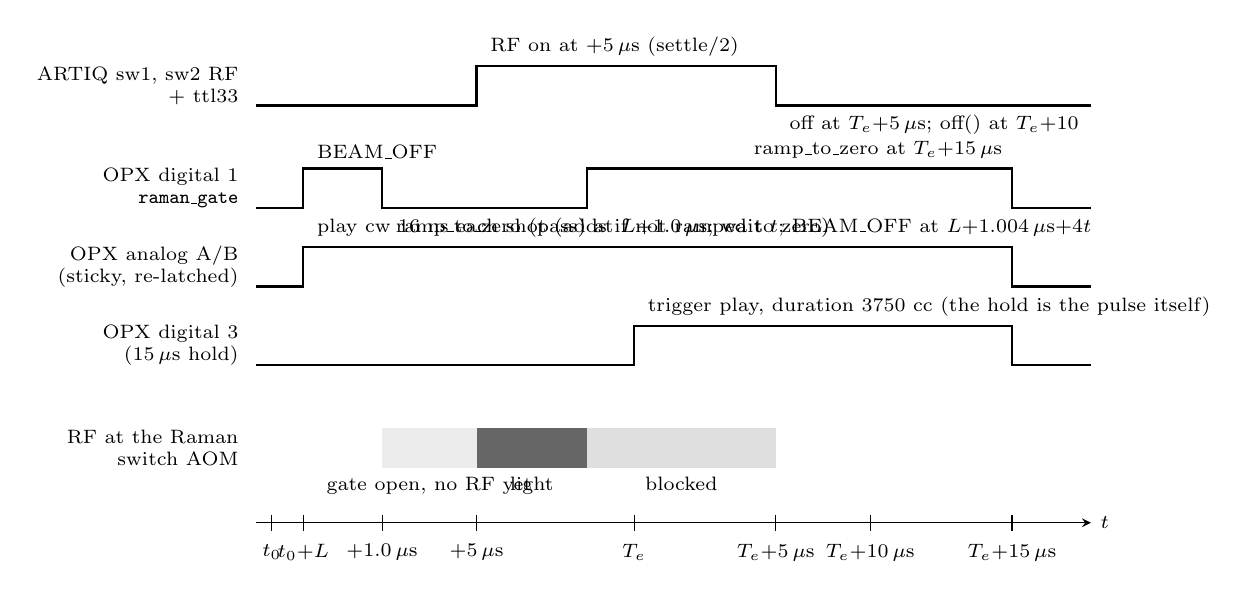
\begin{tikzpicture}[>=stealth, font=\scriptsize, x=1cm, y=1cm]
  \node[anchor=east, align=right] at (0.7,4.25) {ARTIQ sw1, sw2 RF\\+ ttl33};
  \node[anchor=east, align=right] at (0.7,2.95) {OPX digital 1\\\code{raman\_gate}};
  \node[anchor=east, align=right] at (0.7,1.95) {OPX analog A/B\\(sticky, re-latched)};
  \node[anchor=east, align=right] at (0.7,0.95) {OPX digital 3\\(15\us\ hold)};
  \node[anchor=east, align=right] at (0.7,-0.35) {RF at the Raman\\switch AOM};
  % ARTIQ RF: on at 3.6 (+5us), off at 7.4 (Te+5)
  \draw[thick] (0.8,4.0) -- (3.6,4.0) -- (3.6,4.5) -- (7.4,4.5) -- (7.4,4.0) -- (11.4,4.0);
  \node[anchor=south west] at (3.65,4.5) {RF on at +5\us\ (settle/2)};
  \node[anchor=north west] at (7.45,4.0) {off at $T_e$+5\us; off() at $T_e$+10};
  % raman_gate: BEAM_OFF at L (1.4), ramp_to_zero at 2.4 (L+1.0us), BEAM_OFF at 5.0, ramp_to_zero at 10.4 (Te+15)
  \draw[thick] (0.8,2.7) -- (1.4,2.7) -- (1.4,3.2) -- (2.4,3.2) -- (2.4,2.7) -- (5.0,2.7) -- (5.0,3.2) -- (10.4,3.2) -- (10.4,2.7) -- (11.4,2.7);
  \node[anchor=south west] at (1.45,3.2) {BEAM\_OFF};
  \node[anchor=north west] at (2.45,2.7) {ramp\_to\_zero (pass) at $L$+1.0\us; wait $t$; BEAM\_OFF at $L$+1.004\us+4$t$};
  \node[anchor=south east] at (10.4,3.2) {ramp\_to\_zero at $T_e$+15\us};
  % analog: latch at 1.4, ramp_to_zero at 10.4
  \draw[thick] (0.8,1.7) -- (1.4,1.7) -- (1.4,2.2) -- (10.4,2.2) -- (10.4,1.7) -- (11.4,1.7);
  \node[anchor=south west] at (1.45,2.2) {play cw 16 ns each shot (adds if not ramped to zero)};
  % digital 3: 5.6 -> 10.4
  \draw[thick] (0.8,0.7) -- (5.6,0.7) -- (5.6,1.2) -- (10.4,1.2) -- (10.4,0.7) -- (11.4,0.7);
  \node[anchor=south west] at (5.65,1.2) {trigger play, duration 3750 cc (the hold is the pulse itself)};
  % physical: gate open no RF 2.4 -> 3.6 (hatched-ish: lighter), light 3.6 -> 5.0
  \fill[gray!15] (2.4,-0.6) rectangle (3.6,-0.1);
  \fill[black!60] (3.6,-0.6) rectangle (5.0,-0.1);
  \fill[gray!25] (5.0,-0.6) rectangle (7.4,-0.1);
  \node[anchor=north] at (3.0,-0.6) {gate open, no RF yet};
  \node[anchor=north] at (4.3,-0.6) {light};
  \node[anchor=north] at (6.2,-0.6) {blocked};
  \draw[->] (0.8,-1.3) -- (11.4,-1.3) node[right] {$t$};
  \foreach \x/\lab in {1.0/$t_0$, 1.4/$t_0{+}L$, 2.4/+1.0\us, 3.6/+5\us, 5.6/$T_e$, 7.4/$T_e{+}5\us$, 8.6/$T_e{+}10\us$, 10.4/$T_e{+}15\us$} {
    \draw (\x,-1.4) -- (\x,-1.2);
    \node[anchor=north] at (\x,-1.45) {\lab};
  }
\end{tikzpicture}
\caption{The 00e-era handoff. The OPX opened the Raman gate at $t_0 + L +
1.0\us$ but ARTIQ's RF reached the switch AOM only at $t_0 + 5\us$: the first
$4\us - L$ of every exposure had no RF, and the four shortest non-zero
settings (1.07, 2.14, 3.21, 4.28\us) produced no light at all (inferred; it
holds if the committed \code{control.py} was the one running). Also visible:
the 15\us\ hold is the trigger \emph{pulse} itself, the blocks are released by
the sticky end-of-statement rule rather than an explicit pass, the analog
drives are re-latched every shot (safe only because of the trailing
\code{ramp\_to\_zero}), and each exposure carries the 4\nsu\ ramp. Source:
\file{00e\_hello\_atoms\_scan.py} lines 47--94, \file{configuration.py}.}
\label{fig:timing_b}
\end{figure}

What the builder changed relative to 00e: exposure is a \code{pass} play of
exactly $d$ (no ramp, no $+4\nsu$); the analog drives are latched once per
run; the blocks idle low between shots; the hand-back trigger is 200\nsu\
and the hold is a \code{wait} on the switch elements; and the shot values
come from the same shuffled tables as the ARTIQ scan instead of an OPX-side
list that the HDF5 file knew nothing about.

\subsection{Waste and risk, per OPX window}
\label{sec:handoff:waste}

\begin{table}[htbp]
\centering
\scriptsize
\begin{tabular}{@{}llp{7.6cm}l@{}}
\toprule
\# & item & detail & kind \\
\midrule
W1 & overlap 15\us\ vs $\sim$8.5--10\us\ need & CPU reaction ($\sim$4--7\us) + RF fall ($\sim$1\us) + margin; $\sim$5\us\ idle per window, 15\us\ dead on the ARTIQ timeline & waste \\
W2 & handoff settle & 1.35\us\ dead time both sides; the 00e script waited 9.984\us & waste \\
W3 & B5/B6 & two RTIO writes re-asserting a level written 7.5\us\ earlier (\code{off()} bookkeeping) & waste \\
W4 & 2\,s timeout & with a dead job every shot burns 2\,s \textbf{with both switch-AOM RFs ON and the OPX lines idle low (= pass)}: light on the atoms and detector until \code{TriggerTimeout} & waste + physics \\
W5 & aligns & the removed A2 and the trailing \code{wait\_s} align cost a few cycles each & negligible \\
W6 & both RFs on regardless of claims & \code{handoff\_to\_quantum\_machines} turns raman \emph{and} imaging RF on unconditionally, so both blocks are guarded in every window; a raman-only sequence still blocks the imaging switch & design \\
W7 & imaging intensity servo & whether it winds up while its switch is blocked depends on where its photodiode sits; PID clear/override TTLs are dead; M1 & risk (open) \\
W8 & \code{prep\_raman} & 10.7--28.2\,ms per shot (warm-up, shutter, line trigger); necessary, dwarfs W1/W2 & info \\
R1 & handoff leak & ARTIQ RF at +349\,mu vs block complete at $L$ + align + $\sim$1\us\ turn-off: \textbf{up to $\sim$0.65--1\us\ of raman and imaging light} if $L \sim 1\us$; unmeasured & logic-risk \\
R2 & take-back CPU margin & 0.5--3.5\us\ depending on which in-repo per-event cost is right & logic-risk \\
R3 & underflow in the take-back left RF on & fixed: \code{cleanup\_scan\_kernel} now calls \code{imaging.off()}, \code{raman.off()} (\file{base.py} lines 311--316) & fixed \\
R4 & crash left ttl33 HIGH into the next run & fixed: \code{init\_kernel} drops ttl33 after \code{switch\_all\_dds(0)} (\file{base.py} line 180) & fixed \\
R5 & crash-state docstrings & rewritten in \code{control.py} (section~\ref{sec:handoff:crash}), in \code{TTL.py} (\code{wait\_for\_edge}) and in the \code{expt\_params.py} comment block & doc \\
R6 & 00e sticky release timing & the 00d/00f single-shot release relies on the end-of-program ramp & inferred \\
\bottomrule
\end{tabular}
\caption{Waste and risk items from the phase-1 handshake audits
(\code{artiq\_handshake.md} \S4, \code{customer\_handoff.md} \S3).}
\label{tab:waste}
\end{table}

\subsection{Unmeasured assumptions (the M1 list)}
\label{sec:handoff:m1}

Everything below must be seen on a scope with no atoms before this design
is trusted:

\begin{enumerate}[nosep]
  \item Trigger $\to$ block-complete latency versus the 350\nsu\ assumption.
    Both beams leak if it fails (R1). The previous design (RF at settle/2 =
    5\us) was safe by construction; the current one is faster and unproven.
  \item Hand-back CPU slack: the VERBOSE \code{aprint} in
    \code{wait\_for\_quantum\_machines\_handback} is the measurement and has
    never been run. Expected 4--7\us\ against the 7.5\us\ slot.
  \item Digital line state after \code{job.halt()} mid-block. If a line stays
    HIGH, every following non-OPX run has that switch AOM's RF blocked.
  \item QOP acceptance of port-less sticky digital elements
    (\code{raman\_switch}/\code{imaging\_switch} have no analog port). If
    refused, add the dummy analog port as QM's template did.
  \item Run once with \emph{no} OPX job: every shot must end in
    \code{TriggerTimeout}, never in a false edge on ttl41.
  \item Whether the sticky analog hold keeps the IF tone \emph{oscillating}
    (the lab saw RF on the AOs in 00d/00e, so empirically yes; one explicit
    trace).
  \item The imaging intensity servo while its switch is blocked (W7).
\end{enumerate}

\subsection{End states on crash and abort (corrected)}
\label{sec:handoff:crash}

The old docstrings said an ARTIQ crash mid-window ``leaves the blocks HIGH
until the ARTIQ process exits''. That is not what the emitted program does:
after \code{wait\_for\_trigger} the OPX shot has no further dependency on
ARTIQ -- body, A4, 200\nsu\ trigger, \code{wait(3750)}, \code{pass} -- so the
blocks are released 15\us\ after every hand-back whatever ARTIQ does.

\begin{center}\small
\begin{tabular}{@{}p{4.2cm}p{10.4cm}@{}}
\toprule
case & end state \\
\midrule
ARTIQ underflows \emph{before} the handoff & no trigger; OPX parked at \code{wait\_for\_trigger} with blocks at pass; \code{cleanup\_scan\_kernel} drops ttl33; \code{end()} $\to$ \code{finish()} halts the job. Safe. \\
ARTIQ underflows \emph{between} handoff and hand-back & the OPX finishes its shot and releases the blocks at $T_e$+15\us; ARTIQ never runs the take-back. Before the rebuild the raman and imaging RF stayed ON (cleanup only dropped ttl33 and the shutter) and imaging light passed until the next run's \code{init\_kernel}. Now \code{cleanup\_scan\_kernel} also calls \code{imaging.off()} and \code{raman.off()} (one RTIO event each). \\
Hand-back never comes (dead job) & \code{TriggerTimeout} after 2\,s (below); blocks are whatever the dead job left -- HIGH if it died mid-body, until halt. \\
Kernel dies while blocked (uncaught exception, \code{TerminationRequested} from a liveOD abort) & \textbf{the real crash end state:} ARTIQ RF ON on both switch AOMs, ttl33 HIGH, OPX blocks LOW after $T_e$+15\us, OPX tones still on the AOs until the \code{atexit} halt. Raman + imaging light pass until the next run's \code{init\_kernel} (\code{switch\_all\_dds(0)}); before the rebuild that run's first shot also ran with ttl33 HIGH -- the 80/150 AOs routed to a halted OPX, i.e.\ no Raman RF -- until its first \code{cleanup\_scan\_kernel}. Now \code{init\_kernel} drops ttl33 right after \code{switch\_all\_dds(0)}. \code{analyze()} never runs, so \code{finish()} never fetches: OPX data of such a run is lost (the underflow/timeout paths preserve it). \\
\code{scan(raise\_underflow=True)} & no cleanup at all: coils hot, RF on, ttl33 high. Not for use with atoms. \\
\bottomrule
\end{tabular}
\end{center}

\subsection{The \code{TriggerTimeout} path}

\code{wait\_for\_edge(7.5e-6, 2.)} computes \code{t\_deadline = now\_mu() +
seconds\_to\_mu(2.)} and blocks in \code{timestamp\_mu(t\_deadline)}. With no
edge it returns $-1$ after 2.0000013\,s; the cursor is placed at
\code{t\_deadline + 7499}, B1--B4 are written (positive slack $\sim$7.4\us),
then B5/B6, then \code{aprint} and \code{raise TriggerTimeout}. \code{Scanner.scan}
catches it (an own \code{except} clause: the compiler gives a local one type,
so it cannot share the underflow handler's name), runs
\code{cleanup\_scan\_kernel}, sets \code{aborted\_bool}, and ends the run with
the shots taken; with \code{save\_on\_underflow=True} \code{analyze()} still
runs, \code{finish()} fetches what the job streamed, and the missing shots are
NaN with \code{opx\_data\_valid = 0}. The physics cost is W4: 2\,s of light per
failing shot. A shorter timeout (0.2\,s) was recommended; the only legitimately
long OPX body is a feedback loop, and that is 1--2\,ms.

\section{Data containers}
\label{sec:data}

OPX results reach the run file through the same \code{DataVault} containers
every kexp experiment uses, so \code{atomdata} sees them as ordinary
\code{ad.data.<key>} arrays, unshuffled with everything else. This section
follows one value from \code{qua.save} to \code{ad.data.apd\_qm}.

\subsection{DataVault shapes}
\label{sec:data:shapes}

\code{add\_data\_container(per\_shot\_shape, dtype)} dispatches to one of six
concrete classes by (ndim $\in \{1, 2\}$) $\times$ (float64, int32,
int64).\footnote{\file{wax/waxx-src/waxx/config/data\_vault.py},
\code{add\_data\_container} and the \code{\_registry} dict.} At
\code{data.init()} (inside \code{finish\_prepare\_wax}) every container's
\code{\_run\_data} is patterned to \code{(*xvardims, *per\_shot\_shape)} and
\emph{trailing} size-1 per-shot axes are dropped:

\begin{center}\small
\begin{tabular}{@{}lll@{}}
\toprule
declared per-shot shape & \code{xvardims} & \code{\_run\_data.shape} \\
\midrule
\code{(1,)} & \code{[20]} & \code{(20,)} \\
\code{(4,)} & \code{[20]} & \code{(20, 4)} \\
\code{(N, m)} & \code{[10, 5]} & \code{(10, 5, N, m)} \\
\code{(1,)}, 3 repeats of 10 values & \code{[30]} & \code{(30,)} -- repeats fold into the axis \\
\bottomrule
\end{tabular}
\end{center}

A kernel-written container is filled per shot by \code{put\_shot\_data}: the
cell index is the tuple of \emph{host} xvar counters, i.e.\ the execution-order
\code{ndindex} tuple (\code{\_put\_shot\_data\_to\_run\_data}). The OPX
containers are never touched on the kernel; they stay zero with
\code{\_data\_gotten = False} until \code{end()}.

\subsection{Streams $\to$ buffers $\to$ \code{fill\_containers} $\to$ unshuffle}
\label{sec:data:fill}

On the OPX side every \code{measurements} key is one output stream. The
context declares it on first use, and \code{ctx.measure(key)} / \code{ctx.save(key,
expr)} emit \code{qua.save(var, stream)} once per value.\footnote{\file{context.py},
\code{\_get\_stream}, \code{measure}.} In \code{stream\_processing} the builder
groups the saves per shot:

\begin{lstlisting}[style=qua]
stream.buffer(n).save_all(key)               # per-shot shape (n,)   -> fetched as (N_shots, n)
stream.buffer(n2).buffer(n1).save_all(key)   # per-shot shape (n1, n2) -> (N_shots, n1, n2): saves come row-major
\end{lstlisting}

\code{save\_all} keeps the history; \code{fetch\_all()} returns a structured
array whose \code{['value']} field is stripped. Then
\code{OPXManager.fill\_containers} (a static, side-effect-free function, so it
is tested without a job):\footnote{\file{manager.py}, \code{fill\_containers}.}

\begin{lstlisting}[style=py]
n_valid = min(counts[k] for k in seq.measurements)          # smallest stream count
for key, shape in seq.measurements.items():
    target = np.full((n_shots, *shape), np.nan)              # NaN = the OPX never ran this shot
    vals = fetched[key].reshape(-1, *shape)
    if key produced by ctx.measure:  vals = demod2volts(vals, t_integration_s)   # volts; else raw
    target[:n] = vals[:n]
    dc._run_data = target.reshape(dc._run_data.shape)         # execution order -> (*xvardims, *shape), C order
    dc._data_gotten = True
mask[:n_valid] = 1                                           # opx_data_valid
\end{lstlisting}

A C-order reshape of \code{(n\_shots, ...)} into \code{(*xvardims, ...)} puts
flat index $k$ at \code{np.unravel\_index(k, xvardims)}, which is the
\code{ndindex} tuple, which is the counter tuple the kernel path would have
used. So at \code{end\_wax} an OPX container is indistinguishable from a
kernel-written one, and the single server-side unshuffle
(\code{Dealer.\_unshuffle\_ndarray} along every leading axis whose length is
in \code{sort\_N}) is correct for both -- the offline check of
section~\ref{sec:xvars:check} verified this cell for cell.

\paragraph{Volts conversion.} \code{demod2volts(raw, t) = 4096 $\cdot$ raw /
t\_ns}, the same as \code{qualang\_tools.units.unit.demod2volts} without
\code{single\_demod}. QM's own scripts for this lab used
\code{single\_demod=True} (a factor 2) on the same \code{integration.full}
measurement; which is right for a bare integration with unit weights has not
been checked against the ARTIQ sampler -- M3. Only streams produced by
\code{ctx.measure} are converted (via the context's \code{\_stream\_roles});
everything saved with \code{ctx.save} is stored raw.

\subsection{\code{opx\_data\_valid} and the shot-index echo}
\label{sec:data:echo}

\code{ad.data.opx\_data\_valid} (int32, one per shot) means ``the OPX streamed
a complete buffer for every declared key on this shot''. Shots the OPX never
ran are NaN in the value containers and 0 here. It does \emph{not} mean the
ARTIQ half of that shot completed: an ARTIQ shot that underflows after the
hand-back still has a valid OPX buffer (the OPX shot ends before its ARTIQ
shot does), and \code{\_shot\_complete\_count} is incremented in
\code{cleanup\_scan\_kernel}, after the shot.

The \textbf{shot-index echo}: right after \code{wait\_for\_trigger} the
builder saves the QUA \code{shot} counter into a dedicated stream,
\code{opx\_shot\_index} (\code{save\_all}, one int per shot, no buffer);
\code{fill\_containers} checks the fetched echo equals \code{arange(n)},
prints a loud \code{***} line naming the first mismatching shot and cuts the
valid mask there (values are kept as fetched).\footnote{\file{builder.py},
\code{SHOT\_INDEX\_KEY}; \file{manager.py}, \code{fill\_containers}.} This is
the only detector for a desynchronised counter
(section~\ref{sec:xvars:check}); before the rebuild there was none.

\subsection{2-D, int and host-filled containers; timestamps}
\label{sec:data:kinds}

A sequence declares its data in four kinds:\footnote{\file{sequence.py},
\code{Stream}, \code{resolve\_stream}, \code{OPXSequence}.}

\begin{center}\small
\begin{tabular}{@{}llll@{}}
\toprule
declaration & container dtype & filled from & volts? \\
\midrule
\code{measurements=\{key: N\}} & float64 (missing: NaN) & stream, \code{buffer(N)} & only if from \code{ctx.measure} \\
\code{measurements=\{key: (N, m)\}} & float64 & stream, \code{buffer(m).buffer(N)} & only if from \code{ctx.measure} \\
\code{measurements=\{key: Stream(N, int)\}} & int64 (missing: $-1$) & stream (a QUA int, or a timestamp stream) & no \\
\code{host\_data=\{key: shape\}} & float64 (\code{Stream(..., int)}: int64) & \code{ctx.host\_data(key, values)} at trace time, written at \code{finish()} & no \\
\bottomrule
\end{tabular}
\end{center}

A callable value (\code{lambda p: p.N\_pulses}, or \code{lambda p:
Stream(p.N\_pulses, int)}) is resolved at \code{use()} against the live
params; shapes are 1-D or 2-D (DataVault containers are). Missing shots are
NaN in float containers and \code{INT\_MISSING} $= -1$ in int containers;
\code{opx\_data\_valid} is the authoritative flag. \textbf{Timestamps}: \code{play(...,
timestamp\_stream=s)} and \code{measure(..., timestamp\_stream=s)} record the
statement's start time in clock cycles from program start (QOP $\ge$ 2.2, int
stream); in the context a \code{timestamp\_key} argument on
\code{ctx.raman\_pulse}/\code{ctx.imaging\_pulse}/\code{ctx.measure} names the
declared int key and counts as one save on it. They are what the feedback
port uses to know the \emph{actual} pulse start times
(section~\ref{sec:feedback:schedule}). A timestamped pulse that is skipped
on some shots by its per-shot duration guard ($d < 16\nsu$) saves the
placeholder \code{TIMESTAMP\_SKIPPED} $= -1$ in the \code{else\_} branch
instead, so the stream keeps exactly one entry per declared save and the
buffers stay aligned; a constant zero-length timestamped pulse is refused
at trace time, and a \code{measure()} key cannot double as a timestamp key.

\paragraph{Validation.} \code{\_validate} requires, per key, that the traced
saves per shot equal \code{prod(shape)}; saves inside \code{ctx.for\_range(n)}
count $n$ times; timestamp plays count as saves; and every declared
\code{host\_data} key must have been written with \code{ctx.host\_data}. A
mismatch is a trace-time \code{RuntimeError} naming both numbers.

\subsection{What the run file holds, and how to read it back}
\label{sec:data:file}

Besides the containers under \code{data/}, the OPX adds three attributes
through \code{expt.\_extra\_file\_texts}, which \code{end\_wax} ships in the
\code{END\_RUN} payload and the liveOD \code{DataSaver} writes as one HDF5
attribute per key:\footnote{\file{manager.py} (\code{QUA\_SOURCE\_ATTR});
\file{wax/waxx-src/waxx/base/expt.py} \code{\_serialize\_end\_payload};
\file{wax/waxa-src/waxa/data/data\_saver.py} \code{\_write\_end\_run\_outputs}.}

\begin{center}\small
\begin{tabular}{@{}lp{10.5cm}@{}}
\toprule
attribute & content \\
\midrule
\code{opx\_qua\_program} & \code{generate\_qua\_script(prog, config)}: the full QUA program text including every \code{declare(..., value=[...])} per-shot array (in cc / integer Hz / fixed, keyed by value) and the config dict (ports, IFs at the first executed shot's transition, amplitudes, acquire and integration windows). Generated \emph{before} \code{open\_qm}; the simulated (sliced) program is not saved. \\
\code{opx\_machine} & JSON of the component tree (\code{Machine.to\_dict()}): every element as a dataclass dict plus \code{\_\_class\_\_}, the machine's \code{extra} dict (the transition and windows it was compiled from, the handshake windows, the guarded channels), the qm-qua version (from package metadata, no \code{qm} import) and a generation timestamp. \\
\code{opx\_shot\_tables} & JSON: \code{sequence}, \code{n\_shots}, \code{xvardims}, \code{xvarnames}, the sorted \code{accessed} keys, \code{config\_time\_params}, \code{columns} (the SI value of every accessed key on every shot, execution order), \code{shot\_arrays} (shapes), the resolved \code{measurements} and \code{host\_data} specs, \code{qm\_version}, \code{host}, \code{cluster}, \code{simulate}, and \code{job\_id} once the job is executed (the text is written again then). \\
\bottomrule
\end{tabular}
\end{center}

Reading it back:

\begin{lstlisting}[style=py]
import json, h5py, numpy as np
from kexp import atomdata

ad = atomdata(run_id, roi_id='auto')
valid = ad.data.opx_data_valid.astype(bool)          # (*xvardims,)
apd = ad.data.apd_qm                                  # (*xvardims, 4), volts, NaN where invalid

with h5py.File(ad.run_info.filepath[0], 'r') as f:
    qua_text = f.attrs['opx_qua_program']             # str: the exact program
    machine = json.loads(f.attrs['opx_machine'])      # dict: elements, ports, sticky, IFs
    tables = json.loads(f.attrs['opx_shot_tables'])   # dict: 'columns' -> {key: [SI per shot, execution order]}

# the value each accessed parameter had on OPX shot k (execution order);
# to place it on the unshuffled grid use data/sort_idx, data/sort_N as DataSaver does
t_pulse_exec = np.asarray(tables['columns']['t_raman_pulse'])
\end{lstlisting}

\code{waxa} has no reader for these attributes yet; they are write-only
provenance, by design small (accessed keys only).

\paragraph{Two pre-existing footguns of the per-axis scheme, not OPX-specific
but relevant.} (i) At \code{END\_RUN} the server unshuffles \emph{any}
numeric array-valued param whose axis length equals one of \code{sort\_N}
(\code{data\_saver.py} lines 730--744): an unrelated array stashed on
\code{ExptParams} with a matching length is silently permuted. Do not stash
per-shot tables on \code{ExptParams}; use \code{host\_data}. (ii) A container
whose values are all exactly zero never sets \code{\_data\_gotten} and is
never written, so ``not saved'' and ``all zeros'' are indistinguishable for
kernel-written containers; the OPX path sets \code{\_data\_gotten = True}
explicitly.

\section{Parameters in the loop, and what happens if they change}
\label{sec:midloop}

The user's question, verbatim: \emph{``how are warnings/errors implemented if
parameters are changed mid-loop? Should we be reassigning to xvar list
elements? Is this what we are doing?''}

\subsection{The short answer}

\textbf{No, and no.} Nothing in the tree reassigns to xvar list elements, and
nothing should. On the ARTIQ side the scanned attribute \code{self.p.<key>} is
a \emph{scalar} that the host \emph{reassigns} every shot from the (repeated,
shuffled) value list -- \code{vars(self.params)[xvar.key] =
xvar.values[xvar.counter]} -- and the kernel copy is refreshed by a generated
writer whose source is \code{self.params.<key> = value}
(section~\ref{sec:xvars:scanloop}). The list \code{xvar.values} is written
exactly once, by \code{shuffle\_xvars} at \code{finish\_prepare}, and only
\emph{read} thereafter; after the run \code{cleanup\_scanned} replaces the
scalar with the whole execution-order list so \code{atomdata} sees arrays.
On the OPX side nothing is reassigned at all: the whole column is baked into
a QUA array at \code{finish\_prepare} and read as \code{arr[shot]}
(section~\ref{sec:xvars:resolve}).

So the two machines agree by construction because both derive every shot's
value from the same frozen list in the same order -- not because anything
checks it at run time. What \emph{is} checked, and what is not, follows.

\subsection{What is protected: the liveOD Adjust panel}
\label{sec:midloop:adjust}

The only live-change path the framework offers is \code{adjust()}: the liveOD
Adjust panel rewrites host params between shots. Runtime:
\code{\_notify\_shot\_complete} receives the current values with each
\code{SHOT\_COMPLETE} reply, and \code{update\_params\_from\_xvars} applies them
on the \emph{next} shot before \code{compute\_derived}, so an adjusted value
takes effect one shot later and flows into derived quantities.\footnote{\file{wax/waxx-src/waxx/base/expt.py}
\code{\_notify\_shot\_complete}, \code{apply\_pending\_adjust\_values}.} The OPX
cannot follow it: its values were baked. So \code{check\_live\_adjust\_conflicts(expt,
tables)} refuses the run at \code{on\_finish\_prepare}:\footnote{\file{manager.py}
lines 67--96; \code{derived\_dependents} in \file{params\_bridge.py}.}

\begin{itemize}[nosep]
  \item \code{RuntimeError} if an adjust key is in \code{tables.accessed}
    (the sequence read \code{ctx.p.<key>}): ``the OPX baked its per-shot
    values at finish\_prepare and would not follow the Adjust panel. Drop the
    adjust() or scan it as an xvar.''
  \item \code{RuntimeError} if \code{derived\_dependents(expt, key, accessed)}
    is non-empty: nudging the key by 1\,\% on a working copy and re-running
    \code{compute\_derived}/\code{compute\_new\_derived} moves an accessed
    column. This is ``a safety net, not a proof'': a derived value that only
    reacts to a larger change, or through a threshold, is missed.
  \item The config-time keys (section~\ref{sec:program:config}) are in
    \code{accessed} too, so adjusting the acquire window or a handshake
    number is refused the same way.
\end{itemize}

Two caveats. The check runs \emph{after} \code{finish\_prepare\_wax} has
claimed a run id and created the file, so a refused run leaves a stub file
(\code{run\_complete = False}) that nothing aborts (the config-time
\emph{xvar} refusal, by contrast, already runs at \code{use()}, before
\code{INIT\_RUN}). And Adjust-panel changes
are not recorded per shot anywhere in the saved data (the code says so:
``Values changed in the Adjust panel between shots will NOT be reflected in
saved data''); the final \code{params/} group holds whatever value the param
had at \code{end()}. That is a provenance gap independent of the OPX.

\subsection{What is not protected}
\label{sec:midloop:holes}

\begin{center}\small
\begin{tabular}{@{}p{4.6cm}p{9.9cm}@{}}
\toprule
hole & what happens \\
\midrule
a kernel writes \code{self.p.<x> = ...} inside \code{scan\_kernel} & effective for the rest of that shot; overwritten at the top of the next by \code{write\_host\_params\_to\_kernel}; copied back to the host at kernel exit by ARTIQ's attribute write-back, so the saved \code{params/} can hold a kernel-mutated value for a non-scanned param with no warning. The OPX used the baked value. The lab counts $\sim$23 such writes (\code{p.t\_tof} in 7 files, ...). \\
an RPC mutates params mid-run & the ARTIQ feedback experiment does this every shot (\code{self.p.omega\_pulse\_list = self.get\_new\_pulse\_list(...)}, \code{t\_raman\_pulse\_list}). These are arrays, so \code{build\_shot\_tables} never sees them: no column, no conflict check, no route to the OPX except \code{shot\_array}/\code{host\_data}. \\
host edits after \code{finish\_prepare} & anything an experiment sets on \code{self.p} after \code{super().finish\_prepare()} diverges silently; nothing diffs at shot time. \\
\code{compute\_new\_derived} reading non-param state & the sweep calls it on the working copy; an attribute of the experiment that the kernel later changes, or a random draw, is whatever it was at \code{finish\_prepare}. \\
Adjust panel on the ARTIQ side & allowed, applied next shot, never recorded per shot. \\
counter desynchronisation & one trigger per shot is the only ARTIQ$\leftrightarrow$OPX index link; detected after the fact by the shot-index echo (section~\ref{sec:data:echo}), never prevented. \\
\bottomrule
\end{tabular}
\end{center}

\subsection{Why \code{kernel\_invariants} cannot do this job}

ARTIQ's \code{kernel\_invariants} marks an attribute as never changing while
the kernel runs: loads are hoisted, an assignment in a kernel is a
\emph{compile} error, and the attribute is excluded from write-back. It is an
optimisation and a compile-time write guard on device objects
(\code{Feedback} declares 16, the LUTs and calibrations). Anything on
\code{ExptParams} can never be invariant, because the generated writers
assign \code{self.params.<key>} every shot and \code{vars(self.params)} is
archived through write-back. So it cannot be the mechanism that keeps a
scanned parameter fixed within a shot.\footnote{\file{artiq/doc/manual/compiler.rst}
lines 229--273; \file{k-exp/kexp/util/profiling/KERNEL\_INVARIANTS\_PLAN.md}.}

\subsection{Proposed guards (not implemented)}
\label{sec:midloop:guards}

In order of leverage; each is a small change and none is in the rebuild
scope:

\begin{enumerate}[nosep]
  \item \textbf{Freeze-and-diff.} Keep \code{tables} after the trace and, in
    \code{Scanner.update\_params\_from\_xvars} (a kexp hook), compare the
    live scalars for every key in \code{tables.accessed} against
    \code{tables.column(key)[np.ravel\_multi\_index(counters, xvardims)]}.
    Mismatch $\to$ \code{RuntimeError} naming the key, the shot and both
    values. One dict compare per shot, negligible next to the $\sim$270 RPC
    fetches. Always-on for accessed keys.
  \item \textbf{Refuse kernel/RPC writes to accessed params.} At trace time,
    \code{inspect.getsource} every \code{@kernel}/\code{@rpc} method of
    \code{type(expt)} for \code{self.p.<key> =} / \code{self.params.<key> =}
    with \code{<key>} in \code{accessed}, and raise. Cannot catch
    \code{setattr}; catches the 23 known direct writes.
  \item \textbf{End-of-run hash.} At \code{finish()}, rebuild the accessed
    columns from the final host params (after write-back, before
    \code{cleanup\_scanned}) and compare with the tables the program was built
    from; on mismatch print \code{***} and write
    \code{f.attrs['opx\_params\_drift']}. The honest ``the OPX did not run what
    the file says'' flag.
  \item \textbf{Run the guards before \code{INIT\_RUN}}, or call
    \code{abort\_run} on failure, so a refused run does not burn a run id.
  \item \textbf{Record Adjust values per shot} (ARTIQ side): a container per
    adjust key written from \code{apply\_pending\_adjust\_values}.
  \item \textbf{Counter handshake, stronger form:} ARTIQ pushes the shot index
    through an input stream and the OPX assigns its counter from it -- the
    route reserved at the top of the shot loop, not simulatable.
\end{enumerate}

The \code{opx\_shot\_tables} provenance attribute (section~\ref{sec:data:file})
is item 4 of the audit's list and is implemented: with it, any later reader
can reconstruct exactly what the OPX used without parsing the QUA text.

\section{Tutorial: adding a new per-shot sequence}
\label{sec:tutorial}

\subsection{From a physics description to a sequence}

Take a Ramsey measurement: two $\pi/2$ pulses separated by a variable delay,
with a scanned two-photon detuning, read out by the ARTIQ camera after the
hand-back. In words: \emph{reset the two-photon phase, expose for
$t_\pi/2$, wait $t_{\rm Ramsey}$, expose for $t_\pi/2$ again, at a transition
frequency offset by $\delta$}. The ARTIQ half of the shot (tweezer prep,
\code{prep\_raman}, handoff, hand-back, TOF, image) is the reference
experiment's \code{scan\_kernel} unchanged; the OPX half is:

\begin{lstlisting}[style=py]
# kexp/experiments/opx_sequences/ramsey.py
from kexp.control.opx import opx_sequence, KexpShotContext

@opx_sequence('ramsey_raman', claims=('raman',))
def ramsey_raman(ctx: KexpShotContext):
    ctx.set_transition('raman', ctx.p.frequency_raman_transition
                                 + ctx.p.frequency_ramsey_detuning)   # per shot if scanned
    ctx.raman_phase_reset()                                          # both drives, phase 0 at the next play/align
    ctx.raman_pulse(ctx.p.t_raman_pi_pulse / 2)                      # host arithmetic on a ParamRef
    ctx.wait_s(ctx.p.t_ramsey)
    ctx.raman_pulse(ctx.p.t_raman_pi_pulse / 2)
\end{lstlisting}

And in the experiment's \code{prepare()}:

\begin{lstlisting}[style=py]
self.p.frequency_ramsey_detuning = 0.            # must exist on ExptParams before xvar()
self.xvar('frequency_ramsey_detuning', np.linspace(-50.e3, 50.e3, 21))
self.p.t_ramsey = 200.e-6
self.opx.use(ramsey_raman)
self.finish_prepare(shuffle=True)
\end{lstlisting}

The rules the decorator enforces: \code{claims} lists every role the body
touches (\code{'raman'}, \code{'imaging'}); \code{measurements} lists every
key the body saves into and the per-shot shape; \code{host\_data} lists the
host-filled keys; a body that violates any of these fails at trace time,
inside \code{finish\_prepare}, before the run starts (but after the run id is
claimed -- section~\ref{sec:midloop:adjust}).

\subsection{What each \code{ctx} call emits}
\label{sec:tutorial:macros}

\begin{table}[htbp]
\centering
\scriptsize
\begin{tabular}{@{}p{4.6cm}p{9.9cm}@{}}
\toprule
\code{ctx} call & QUA emitted (\code{d} = clock cycles: a Python int if constant, \code{arr[shot]} if per shot, or a QUA int expression) \\
\midrule
\code{ctx.raman\_pulse(t)} & \code{play('pass', 'raman\_switch', duration=d); play('block', 'raman\_switch')}. Constant $d = 0$: nothing. Per-shot $d$: both plays inside \code{with if\_(d >= 4)}. \\
\code{ctx.raman\_pulse(t, phase\_reset=True)} & \code{reset\_if\_phase('raman\_80'); reset\_if\_phase('raman\_150'); align('raman\_80', 'raman\_150', 'raman\_switch')} then the two plays, nothing in between on the switch element. The reset takes effect at that align. Inside the \code{if\_} guard when $d$ varies. \\
\code{ctx.raman\_pulse(t, timestamp\_key='k')} & the pass play gets \code{timestamp\_stream=<stream k>}; counts as one save on \code{k} (a declared int key); on shots where the guard skips the pulse, \code{save(-1, stream k)} in the \code{else\_} branch. \\
\code{ctx.raman\_pulse(d\_qua, min\_cc=k)} & for a QUA-expression duration with a host-known lower bound $k \ge 4$\,cc: the \code{if\_} guard is omitted, so the pulse (and its phase-reset align) is emitted with no run-time branch and no implicit align. Ignored for host values; $k < 4$ is refused. \\
\code{ctx.imaging\_pulse(t, timestamp\_key=None, min\_cc=None)} & same on \code{imaging\_switch} (no phase reset: it has no analog drives). \\
\code{ctx.raman\_phase\_reset()} & \code{reset\_if\_phase} on both drives, no align (takes effect at the next play/align on each element). \\
\code{ctx.set\_frequency('raman', f, which=None, keep\_phase=False)} & \code{update\_frequency(el, hz)} on the selected drive(s): \code{which} picks one drive by index or element name (default: every drive of the role); \code{f} in Hz as a number, a \code{ParamRef} (per shot) or a QUA int expression (integer Hz, e.g.\ a table cell \code{if80T[d]}); marks the role for IF restore after the body. \\
\code{ctx.set\_transition('raman', f)} & \code{update\_frequency} on both drives with \code{transition\_to\_ifs(f)} (the \code{RamanBeamPair} split); per shot if \code{f} varies. \\
\code{ctx.set\_transition\_offset('raman', df\_hz)} & for a QUA int \code{df}: \code{update\_frequency(el, IF0\_el + Cast.mul\_int\_by\_fixed(df, slope\_el))} per drive, \code{IF0\_el} the run transition's IF and \code{slope\_el} = $\partial\,\mathrm{IF}_{el}/\partial f$ from \code{transition\_to\_ifs} at $f \pm 1$\,kHz, asserted linear to $10^{-9}$ over $\pm 2$\,MHz; for a host value or \code{ParamRef}: the exact split at $f_{\rm run} + \delta f$, per shot. Refuses a transition that varies per shot. \\
\code{ctx.transition\_offset\_terms('raman')} & nothing on the OPX: returns \code{\{element: (IF0 int Hz, slope)\}} for the run's transition, the terms \code{set\_transition\_offset} uses, so a sequence can form the integer IFs itself (host tables, exact applied frequency) and apply them with \code{set\_frequency(..., which=element)}. Same run-constant transition rule. \\
\code{ctx.frame\_rotation('raman', turns)} & \code{frame\_rotation\_2pi(x, el)} per drive. \\
\code{ctx.reset\_frame('raman')} & \code{reset\_frame(el)} per drive. \\
\code{ctx.measure(key, role='imaging', expose=True, t\_expose=None, timestamp\_key=None, expose\_timestamp\_key=None)} & \code{align('imaging\_switch', 'apd')}; if \code{expose}: \code{play('pass', 'imaging\_switch', duration=d); play('block', ...)} with $d$ = \code{t\_expose} or the config acquire length; then \code{measure('acquire', 'apd', integration.full('integration\_window', v, 'out1')); save(v, stream)}. Returns the QUA fixed \code{v} (one per key). \code{expose=False}: the ADC window runs with the beam blocked (a dark shot). \code{timestamp\_key} timestamps the measure, \code{expose\_timestamp\_key} the exposure's pass play (each one save on a declared int key). Refused on a key declared as an int stream. \\
\code{ctx.wait\_s(t)} & \code{align(); wait(d, <every element the map names>)}; a constant 0 emits nothing; a per-shot column containing 0 is guarded with \code{if\_(d >= 4)}. \\
\code{ctx.wait\_cc(d, *names)} & raw \code{wait(d, *elements)} on the named roles/elements only (at least one name); \code{d} a Python int ($0$ or $\ge 4$) or a QUA int. \\
\code{ctx.align(*names)} & \code{align(...)}; role names translate to their switch element; no args = global. \\
\code{ctx.handback\_to\_artiq()} & \code{align(); play('trigger', 'artiq\_handback'); wait(3750, switches); play('pass', ...)}. Auto-appended if the body never calls it; must be the body's last act on the beams. \\
\code{ctx.stream(key)}, \code{ctx.save(key, expr)} & \code{qua.save(expr, stream)}; one save per call, multiplied by enclosing \code{for\_range} counts. \\
\code{with ctx.for\_range(n) as i:} & \code{with for\_(i, 0, i < n, i + 1):}; \code{n} a Python int or a run-constant \code{ParamRef} (\code{ctx.const} rules); a QUA bound is refused (use \code{ctx.qua.for\_} and a fixed declared shape). \\
\code{ctx.shot\_array(key, values, dtype=float)} & one \code{declare(int|fixed, value=flat)}; \code{.at(i)} $\to$ \code{arr[ctx.shot * M + i]} (\code{arr[ctx.shot + i]} when $M = 1$). \\
\code{ctx.host\_data(key, values)} & nothing on the OPX; values go to the declared container at \code{finish()}. \\
\code{ctx.elements(role)} & \code{dict(switch=..., analog=(...), measure=...)} -- the element names, for \code{ctx.qua} code. \\
\code{ctx.const(x)}, \code{ctx.cc(t)}, \code{ctx.hz(f)}, \code{ctx.f(x)} & host-side resolution (section~\ref{sec:xvars:resolve}); \code{cc}/\code{hz}/\code{f} pass a QUA expression through unchanged; \code{const} refuses one. \\
\code{ctx.qua}, \code{ctx.shot}, \code{ctx.n\_shots} & the \code{qm.qua} module (imported on first access), the loop counter, the shot count. \\
\bottomrule
\end{tabular}
\caption{The context API (\file{k-exp/kexp/control/opx/context.py}, after
the rebuild).}
\label{tab:ctx}
\end{table}

\subsection{Per-shot arrays and loops: the feedback shape}

A real-time loop uses these calls together:

\begin{lstlisting}[style=py]
from kexp.control.opx import opx_sequence, Stream
from kexp.control.opx.units import s_to_cc

@opx_sequence('n_pulses_demo', claims=('raman', 'imaging'),
              measurements={'apd_raw': lambda p: int(p.N_pulses),               # (N,) float
                            't_pulse_start_cc': lambda p: Stream(int(p.N_pulses), int)},
              host_data={'t_raman_pulse': lambda p: int(p.N_pulses)})
def n_pulses_demo(ctx):
    N = int(ctx.const(ctx.p.N_pulses))                       # run-level constant
    d_s = draw_durations(ctx, N)                             # host: (n_shots, N) seconds
    d = ctx.shot_array('d_cc', s_to_cc(d_s), dtype=int)      # one flat QUA array
    ctx.host_data('t_raman_pulse', d.values * 4e-9)          # what the OPX will use, rounded
    with ctx.for_range(N) as i:
        ctx.raman_pulse(d.at(i), phase_reset=True, timestamp_key='t_pulse_start_cc')
        v = ctx.measure('apd_raw')                           # exposure + ADC, returns the QUA fixed
        ctx.wait_cc(budget_cc, ctx.elements('raman')['switch'])
\end{lstlisting}

The validator counts one save on \code{apd\_raw} and one timestamp save on
\code{t\_pulse\_start\_cc} per loop iteration, times $N$ -- equal to the
declared shapes. Host-side arithmetic on \code{ParamRef}s is still the way
to build \emph{per-shot scalars}; \code{shot\_array} is for per-shot vectors.

\subsection{Saving variables, timestamps, phase reset, transition offset}

\begin{itemize}[nosep]
  \item \textbf{Saving a QUA variable.} Declare the key in \code{measurements}
    (int or float; e.g.\ \code{'drive\_index': Stream(N, int)}), then
    \code{ctx.save('drive\_index', d)}. Saved raw (no volts conversion). Whole
    arrays cannot be saved: loop with \code{for\_range} and save cells.
  \item \textbf{Timestamps.} \code{timestamp\_key} on a pulse or measure
    records the start cycle of that statement, from program start. Use the
    difference between consecutive timestamps; the absolute value wraps
    modulo $2^{32}$.
  \item \textbf{Phase reset.} \code{reset\_if\_phase} zeroes an element's IF
    phase \emph{at its next play or align}. To have both drives at phase 0
    at the start of a pulse, reset both and align them with the switch
    element immediately before the pass play -- exactly what
    \code{phase\_reset=True} emits. Without the align the two resets take
    effect at each drive's own next statement, which may be shots later.
  \item \textbf{Transition offset.} \code{set\_transition\_offset('raman',
    df)} keeps the \code{RamanBeamPair} ratio split (both drives move, by
    $+0.326\,\delta f$ and $-0.174\,\delta f$ for the 150 and 80\,MHz AOs)
    with a QUA-computed \code{df}. \code{keep\_phase=False} (default): the IF
    phase jumps to what the new frequency would have accumulated since the
    reference; with the per-pulse reset that is irrelevant.
  \item \textbf{Exact integer IFs.} When the analysis must know the applied
    frequency exactly, do the split on the host: \code{terms =
    ctx.transition\_offset\_terms('raman')} gives each drive's integer
    \code{IF0} and slope, a host table of integer IFs per candidate
    frequency becomes a QUA int array, and \code{ctx.set\_frequency('raman',
    table[d], which='raman\_80')} (and the same for \code{raman\_150}) applies
    a row chosen at run time. Streaming the index \code{d} and recording the
    table as host data then fixes the applied two-photon frequency to the Hz
    -- the feedback sequence's pattern (section~\ref{sec:feedback:freq}).
\end{itemize}

\subsection{The escape hatch: \code{ctx.qua}}

\code{ctx.qua} is the \code{qm.qua} module, imported on first access;
\code{ctx.shot} is the loop counter and \code{ctx.n\_shots} the shot count.
Anything the macros do not cover -- \code{declare}, \code{assign},
\code{Math}, \code{Cast}, \code{Util.cond}, \code{if\_} -- is written directly
with it. The rules:

\begin{enumerate}[nosep]
  \item Address elements by \code{ctx.elements(role)}, never by literal
    string, so a renamed element does not silently miss.
  \item Every \code{qua.save} into a declared key must go through
    \code{ctx.save} so the validator counts it; a raw \code{qua.save} on a
    context stream is invisible to it and fails at \code{fill\_containers}
    with a length mismatch.
  \item Nothing may play or measure after \code{handback\_to\_artiq()}
    (\code{\_check\_open}).
  \item Fixed point: every intermediate must stay in $[-8, 8)$; overflow
    wraps silently modulo 16. \code{Math.inv} needs $|x| > 1/8$;
    \code{Math.exp} needs $x < 2.079$; \code{Math.sqrt} non-negative; no
    \code{**}, \code{//}, \code{\%} on QUA expressions; no automatic casting
    (\code{Cast.mul\_int\_by\_fixed} and friends). Section~\ref{sec:feedback:numerics}
    shows the rescalings.
  \item Statements written through \code{ctx.qua} are not in the op log at
    all, so the pulse viewer cannot link them to a source line; a macro's
    play inside your own \code{if\_} is logged as always executing.
\end{enumerate}

\subsection{\code{simulate=True} and the pulse viewer}

\begin{lstlisting}[style=py]
self.opx.use(ramsey_raman, simulate=True, simulate_shots=2, simulate_duration=300.e-6)
self.finish_prepare(shuffle=False)     # deterministic first shots
\end{lstlisting}

At \code{finish\_prepare} the program is re-traced with
\code{skip\_triggers=True} on tables sliced to the first \code{simulate\_shots}
shots (shots then run back-to-back on the simulated timeline), sent to the
QOP simulator, and the pulse viewer opens with every simulated pulse linked
to the sequence line that made it; the process exits before any ARTIQ
hardware runs. Use \code{save\_data=False}. The simulator cannot run
\code{wait\_for\_trigger}, input streams, IO variables or \code{pause}; it does
model computational gaps (verify a \code{wait}'s actual length there). From a
notebook, \code{OPXBench().simulate(seq, shots=2)} does the same without an
experiment.

\subsection{Common errors and what they mean}

\begin{center}\small
\begin{tabular}{@{}p{6.2cm}p{8.3cm}@{}}
\toprule
message (abridged) & meaning \\
\midrule
\code{float() on ctx.p parameter 't\_x': ... a per-shot column, not one number} & you wrote \code{if ctx.p.t\_x > 0} or \code{max(...)}; compute per shot with numpy, or \code{ctx.const} for a run-level toggle \\
\code{ctx.const('N') but it varies per shot (17 .. 20)} & the loop count is scanned; per-shot control flow needs a QUA loop bound, not a Python one \\
\code{uses channel 'imaging' without claiming it} & add it to \code{claims=(...)} \\
\code{measures into 'k', which is not declared in its measurements} & declare the key and its per-shot shape \\
\code{declares 4 saves per shot into 'apd\_qm' but the traced body performs 3} & shape and body disagree; with \code{for\_range} remember saves multiply by $n$ \\
\code{duration for 'raman pulse' rounds to under the OPX minimum of 16 ns} & a nonzero duration below 4 cc; zero is allowed, 1--15\nsu\ is not \\
\code{WARNING: duration ... is off the 4 ns grid by up to 2.0 ns (1.2\%)} & the requested time is not a multiple of 4\nsu; the rounded value is what runs \\
\code{'t\_x' = -inf .. 3 does not fit a 32-bit QUA int (durations of 8.6 s or more ...)} & a seconds-vs-microseconds slip, or a division by a zero parameter \\
\code{'t\_x' is NaN on 3 shot(s) (execution-order index [...])} & a derived parameter left unset on some shots \\
\code{'t\_raman\_pulse' is registered with adjust() but the OPX sequence reads ctx.p.t\_raman\_pulse} & drop the \code{adjust()} or scan it \\
\code{ExptParams has no scalar parameter 'omega\_pulse\_list'} & arrays are not shipped per shot; use \code{shot\_array} \\
\code{['t\_imaging\_pulse\_apd\_abs'] is scanned as an xvar but is compiled into the OPX config once per run} & take one run per value; a config-time parameter \emph{derived} from an xvar fails instead with \code{is a config-time parameter ... but it varies per shot} \\
\code{cannot reach the OPX (host ..., cluster ...) ... Refused in prepare()} & the QMM connection failed in \code{use()}; no run id was claimed \\
\code{the sequence's data shapes changed between use() ... and finish\_prepare} & a parameter a shape depends on was set after \code{self.opx.use(...)}; set it before \\
\code{declares host\_data 't' but never wrote it with ctx.host\_data('t', values)} & every declared host-data key must be written once at trace time \\
\code{ctx.for\_range(n): n must be a Python int ... not a QUA expression} & the loop count is counted at trace time; a run-time bound needs \code{ctx.qua.for\_} \\
\code{*** OPX data present for 12 of 20 shots; the remainder are NaN (int containers: -1) and flagged 0} & an aborted run; not an error \\
\code{*** OPX shot counter echo disagrees with the shot order from shot 7} & the ARTIQ and OPX counters desynchronised (a skipped or doubled handoff); OPX data from shot 7 on is flagged 0 \\
\code{TriggerTimeout: no OPX hand-back edge on ttl41 within the timeout} & the job is not running, not seeing the trigger, or its shot is longer than 2\,s \\
\bottomrule
\end{tabular}
\end{center}

\section{Mapping to QUA and QUAM}
\label{sec:quam}

QUAM (Quantum Abstract Machine, \url{https://qua-platform.github.io/quam/})
is QM's own abstraction layer over QUA: a tree of Python dataclasses rooted
in a \code{QuamRoot}, each component contributing its slice of the QUA config
through \code{apply\_to\_config(config)}, the root emitting the whole dict via
\code{generate\_config()}; channels carry their pulses in an
\code{operations} dict and expose thin wrappers \code{play/measure/wait/align/
update\_frequency/reset\_if\_phase}; the whole tree serialises to JSON with
\code{\_\_class\_\_} stamps. The phase-1 reader went through the QUAM source
(v0.6.0 on \code{main}) and documentation; the comparison below is the
result.\footnote{Phase-1 report \code{quam\_docs.md}; local copies of the
QUAM sources it cites in \code{scratchpad/phase1/quam\_src/}.}

\subsection{Side by side}

\begin{table}[htbp]
\centering
\scriptsize
\begin{tabular}{@{}p{3.6cm}p{3.8cm}p{7.2cm}@{}}
\toprule
ours (\file{kexp/control/opx/components.py}) & QUAM & remarks \\
\midrule
\code{Machine(con, controller\_type, elements, extra)} with \code{validate()}, \code{generate\_config()}, \code{to\_dict()} & \code{QuamRoot} with \code{generate\_config()}, \code{to\_dict()}/\code{save()} & same protocol: template + \code{apply\_to\_config} over elements in order. \code{validate()} checks duplicate names, two elements on one output port, and each element (amplitude $\le$ \code{MAX\_ANALOG\_V}, lengths on the 4\nsu\ grid and $\ge 16\nsu$, window fit). \code{to\_dict()} stamps \code{qm\_qua\_version} (from package metadata) and a timestamp; QUAM stamps \code{\_\_package\_versions\_\_}. No \code{load()}: ours is provenance, not a round trip. \\
\code{Element(name, con, sticky, core)} with \code{op\_name}, \code{pulse\_name}, \code{waveform\_name}, \code{marker\_name}, \code{weight\_name}, \code{labels}, \code{operations()} & \code{Channel} with \code{name} derived from \code{id} or the tree path, \code{operations} dict, \code{pulse\_mapping} & we borrowed the naming rule \code{<element>.<label>.pulse|wf|dm} and \code{<element>.<label>.<weight>.iw} so a second acquire length or a second tone can never collide; names may not contain a dot so the rule stays reversible. Visible element and op names (\code{raman\_switch}, \code{block}/\code{pass}, ...) stay as before (D3). \\
\code{DigitalLine(port, levels=\{'block': 1, 'pass': 0\}, edge\_ns=16)} & \code{Channel} + \code{DigitalOutputChannel} + \code{Pulse(digital\_marker=[(1, 0)])} & QUAM supports purely digital elements explicitly; the hand-back line is \code{levels=\{'trigger': 1\}, edge\_ns=200}. \\
\code{Sticky(duration\_ns, analog=True, digital=True)} & \code{StickyChannelAddon(duration, analog, digital)} & one-to-one, including the \code{analog: True} the QOP demands on digital-only elements. \\
\code{AnalogDrive(port, if\_hz, amplitude\_v, latch\_ns=1000, op='cw')} & \code{SingleChannel(opx\_output, intermediate\_frequency, operations=\{'cw': SquarePulse(...)\})} & QUAM's IF is a static number or a string reference; ours is set per run by the map and re-pointed per shot by the builder from a \code{ParamRef} column -- something references cannot express. \\
\code{IntegratedInput(in\_port, marker\_port, acquire\_ns, window\_start/len\_ns, time\_of\_flight\_ns=200, gain\_db=0, acquire\_op, weight, full\_weight)} & \code{InSingleChannel} + \code{ReadoutPulse} & QUAM's \code{measure} always emits \code{demod.full} with \code{iw1/iw2}; ours emits \code{integration.full} with a cosine-only window (\code{integration\_window}) or the whole pulse (\code{full\_pulse}). A QUAM user would subclass and override. \\
\code{ChannelSpec}/\code{ChannelMap} (roles $\to$ elements, handshake windows, \code{config\_time\_params}, \code{machine}) & no equivalent & kept as the adapter the builder/context use, so \code{ctx.raman\_pulse} etc.\ do not change; \code{\_check\_map\_against\_machine} verifies every element and op the map names exists on the machine (QUAM's \code{play(validate=True)}, done once at \code{use()}). \\
\code{OPXShotContext} macros (\code{raman\_pulse}, \code{measure}, ...) & \code{QuamMacro} / \code{@register\_macro} methods on \code{QuantumComponent}, dispatched by an \code{OperationsRegistry} & the same idea: trace-time functions that emit QUA and may return QUA variables. QUAM's kwargs are per-call overrides, persistent values are dataclass fields; ours are \code{ParamRef} columns. \\
\code{ParamRef}, \code{ShotTables}, \code{build\_shot\_tables} & no equivalent & QUAM has no concept of a scan; its values are single calibrated numbers on the tree. \\
\code{OpLog} + pulse viewer & no equivalent & provenance from pulse to source line. \\
\code{opx\_machine} JSON in the run file & \code{machine.save("state.json")} & same spirit; ours is per run, next to \code{opx\_qua\_program}. \\
\bottomrule
\end{tabular}
\caption{Our component layer against QUAM's. The left column is
\file{kexp/control/opx/components.py} as landed by the rebuild (the spec's
\S2.3), used by \code{build\_machine} in \file{opx\_config.py} and exported
from \code{kexp.control.opx} (\code{from kexp.control.opx import Machine,
DigitalLine, AnalogDrive, IntegratedInput, Sticky}).}
\label{tab:quam}
\end{table}

\subsection{What we borrowed}

\begin{itemize}[nosep]
  \item Elements as objects that generate their own config
    (\code{apply\_to\_config}), instead of the element name appearing in the
    role map \emph{and} the hand-written dict \emph{and} the op log.
  \item The pulse/waveform/weight naming rule.
  \item The sticky addon as a declared, checked property rather than a
    comment.
  \item A machine root with a JSON dump written into the run file as
    provenance, with a version stamp.
  \item \code{validate}-style trace-time checks that an op label exists on the
    element (ours: the role is claimed; the components make the op names
    data).
\end{itemize}

\subsection{What we kept that QUAM does not have}

Per-shot parameter binding to the ARTIQ scan (\code{ParamRef} refusing to
become one number, \code{ctx.const} as the explicit opt-in); the handshake
framing owned by the builder so no sequence can get it wrong; SI units at the
API with grid and range checks; trace-time validation of claims, save counts,
``nothing after hand-back'', cross-run \code{ParamRef} mixing, NaN/inf, live
Adjust conflicts; the op log; the DataVault path with NaN and the validity
mask; and the lab-agnostic import hygiene -- none of
\file{channels/context/builder/manager/params\_bridge/units/components} imports
\code{kexp} or \code{qm} at module level, so \code{kexp} imports on machines
without qm-qua.

\subsection{Why \code{quam} is not a dependency (D3)}

Facts bearing on it: QUAM 0.6.0 requires Python $\ge$3.10, $<$3.15 and
qm-qua $\ge$1.2.3 (our venv: 3.13, qm-qua 1.4.1 -- compatible in principle),
plus \code{typeguard} and \code{qualibrate-config}, neither installed, the
latter pulling in a configuration ecosystem we would never use. QUAM imports
\code{qm} at module import. Its \code{measure} does \code{demod.full}, not
\code{integration.full}. Its references resolve on the host at trace time and
cannot express ``this IF is a per-shot function of a scanned parameter'',
which is our central feature. Its \code{Channel.wait/align} pass channel
objects through \code{str()} (the dataclass repr, not the element name). And
it is in active refactor (v0.5.0 deprecated channel-level port properties,
v0.6.0 deprecated every shaped pulse to \code{quam-builder}). Of its value we
would use perhaps a fifth. So: borrow the shapes into $\sim$300 lines of our
own, and keep the door open by matching them, so that a later switch to real
QUAM -- an Octave or an OPX1000 arriving -- or importing a QUAM-generated
config is mechanical.

\section{The Bayesian feedback loop on the OPX}
\label{sec:feedback}

\statusbox{Status of this port.}{Implemented, speed pass ``3b'' (2026-09-25):
\file{kexp/experiments/opx\_sequences/feedback.py} (\code{make\_feedback\_sequence},
\code{feedback\_constants}, \code{build\_feedback\_shot\_tables},
\code{\_feedback\_body}, \code{feedback\_finish} and the table helpers),
\file{HF\_experiments/feedback/\{expt\_params\_feedback\_opx, feedback\_opx,
feedback\_opx\_deterministic\}.py}, \file{kexp/analysis/feedback\_opx.py}
(\code{FeedbackOPXReplay}, \code{posterior\_update\_fixed\_point\_emulation},
\code{run\_shot\_fixed\_point\_emulation}, \code{true\_bloch\_step}), the
additive host helpers at the end of \file{kexp/base/feedback.py}, and
\file{tests/test\_feedback\_opx.py} (28 items). Offline-tested against the
double-precision ARTIQ posterior; compiled and timed on the QOP simulator
through \code{OPXBench} (section~\ref{sec:feedback:speed}). \textbf{Not run
on hardware.} Every calibration constant it uses was measured through the
ARTIQ path and is a placeholder until re-taken in OPX units
(section~\ref{sec:feedback:calib}). The remesh is a design only
(section~\ref{sec:feedback:remesh}).}

\subsection{The physics in plain words}

Per shot, ARTIQ prepares one spin-polarised ensemble in the HF tweezer
(state $|1,-1\rangle$, Bloch vector $z = +1$) and hands the atoms to the OPX.
The OPX then runs $N$ cycles ($N = $ \code{N\_pulses}: 17 in
\code{feedback\_opx.py}, 9 in the open-loop sweep) of:

\begin{enumerate}[nosep]
  \item a Raman pulse of pre-drawn random duration $\tau_i \in [0.5, 1.0]\,t_\pi$
    (uniform, a pure function of the shot's seed, rounded to the 4\nsu\ clock)
    at the current drive frequency, rotating the Bloch vector about an axis
    that depends on how far the drive is from the true two-photon resonance
    $\omega_0$ (\code{frequency\_raman\_transition} $= 119.4639$\,MHz, $t_\pi =
    7.121\us$, $\Omega/2\pi = 1/(2t_\pi) = 70.2$\,kHz);\footnote{\file{kexp/config/expt\_params.py}
    lines 166, 373.}
  \item a 5\us\ imaging pulse at the ``midpoint'' detuning
    (\code{frequency\_detuned\_hf\_midpoint} $= -519.5$\,MHz), whose dispersive
    signal integrated on the APD is a \emph{weak measurement} of $S_z$: expected
    photon fraction $p_1(z) = \tfrac12(1+z) + (m_f - \tfrac12)(1 - z^2)$,
    $m_f = 0.4719$, which maps $z \in [-1, 1]$ monotonically onto $[0, 1]$
    for any $m_f \in (0.25, 0.75)$; the light also AC-Stark-shifts the levels
    by $f_{LS} = 40.61$\,kHz, a $z$-rotation of $\phi_{LS} = f_{LS}\,t_{\rm img} =
    0.203$ turns per measurement, and scatters photons that shrink the
    transverse spin by $C = 0.62$ (\code{back\_action\_coherence}); $z$ is not
    touched by the measurement;\footnote{\file{HF\_experiments/feedback/expt\_params\_feedback.py}
    lines 43--69; the coherence was fitted with the light shift pinned, and
    the pair is not a self-consistent joint fit (``residuals are still 83x
    the APD error bars'').}
  \item a Bayesian update: for each of $m = 21$ hypotheses $\omega_j$ on a grid
    of $\pm\,$\code{feedback\_guess\_span\_Omega}$\,\Omega$ around the nominal
    resonance plus an integer offset (span 3, offset 2 in \code{feedback\_opx.py}:
    step $0.3\,\Omega = 21$\,kHz), snapped so one point sits exactly on the
    nominal resonance (index \code{zidx}), propagate a Bloch vector through
    the pulse and the measurement, weight it by the Gaussian likelihood of
    the observed photon fraction with the \emph{fixed} detector width
    $\sigma_p = \sigma_n / n = 212.75 / 1336.2 = 0.159$, and drive the next
    pulse at the \textbf{posterior argmax grid point}. The first pulse is
    driven at the grid point nearest \code{feedback\_fractional\_initial\_offset}.
\end{enumerate}

The multi-pulse frequency sensitivity is Ramsey-like: what distinguishes
hypotheses is the phase each accumulates between pulses relative to the
drive. Hence the drive phase at every pulse start must be known.

\subsection{The reset phase model and its consequence (D4)}
\label{sec:feedback:phase}

On ARTIQ the AD9910s run phase-continuous: the physical two-photon drive
phase is the integral of the programmed frequency, and
\code{RamanBeamPair.io\_update\_and\_phase\_update} reconstructs it in integer
FTW arithmetic. The posterior then uses $\phi_{j,i} = \phi_{\rm drive}(t_i) -
\omega_j t_i$. On the OPX the IF phase is a function of absolute time and the
current frequency; instead of rebuilding a tracker, the port uses the
\textbf{reset model}, selected by the integer parameter
\code{feedback\_phase\_model\_reset = 1} (the sequence refuses any other
value):

\begin{quote}
Both Raman analog drives get \code{reset\_if\_phase}, applied by an
\code{align(raman\_80, raman\_150, raman\_switch)} immediately before every
pulse's \code{play('pass', 'raman\_switch', duration=}$\tau_i$\code{)}, so the
two-photon drive phase at every pulse start is 0 (plus a hardware constant
common to all pulses). The posterior uses $\phi_{\rm drive} = 0$ and the
hypothesis term $\phi_{j,i} = -f_j t_i \pmod 1$ (turns), $t_i$ the start of
pulse $i$ from the start of pulse 0. No phase tracker runs on the OPX.
\end{quote}

A constant common phase offset is harmless: the initial state is on the
pole, the measurement is $S_z$, and every operation in the model commutes
with a global $z$-rotation. In the frame rotating at hypothesis $j$ the state
is \emph{static} between pulses: only the pulse \emph{starts} enter the model
(through the azimuth of the rotation axis), and the light-shift and
drive-frame $z$-rotations commute with the free precession. The gaps between
a pulse's end and the exposure, or between the exposure and the next pulse,
do not enter at all -- what must be exact is $t_i$.

\paragraph{The consequence.} With a per-pulse reset, the phase the atoms
accumulate relative to the drive between pulses is $\omega_0\,\Delta t$, not
$(\omega_{\rm drive} - \omega_0)\,\Delta t$:
\[
  f_0 \times 4\nsu = 119.4639\,\mathrm{MHz} \times 4\nsu = 0.478\ \text{turns per clock cycle}.
\]
One cycle of unplanned delay anywhere in the loop rotates every hypothesis
axis by almost half a turn; on ARTIQ the same error costs $\Delta\omega\,\delta
t \sim 10^{-3}$ turns. The reset model trades the tracker for \textbf{exact
knowledge of the pulse-start times in clock cycles}. Three things make that
true:

\begin{enumerate}[nosep]
  \item Every per-step interval is computed on the host from the drawn
    pulse-time list (section~\ref{sec:feedback:schedule}), and the OPX is held
    to it by a per-step wait on the Raman switch element. The Raman play is
    emitted with \code{min\_cc} (the run's shortest drawn duration), so no
    per-shot \code{if\_} guard -- which would add an implicit align and
    non-deterministic cycles -- sits in front of it; the tables refuse a draw
    that rounds below 4\,cc.
  \item The \emph{actual} start of every pulse is recorded with one timestamp
    stream, \code{t\_pulse\_start\_cc} (the Raman \code{'pass'} play) -- the
    only timestamp the model needs. The replay uses the actual times by
    default; the finish hook recomputes the schedule from the saved durations
    and the params and prints a \code{***} line with the largest
    scheduled-vs-actual deviation if any pulse is off it.
  \item The real-time loop uses the \emph{scheduled} times: the host
    precomputes the hypothesis-frame tables from the schedule and ships them
    per shot, so the OPX computes no phase at all.
\end{enumerate}

\subsection{The per-step schedule}
\label{sec:feedback:schedule}

We write $\tau_i$ for the drawn duration of pulse $i$ (the code's
\code{d\_cc[i]}; the code's \code{d} is the \emph{drive index}, below). Per
pulse, in program order, as \code{\_feedback\_body} emits
it:\footnote{\file{kexp/experiments/opx\_sequences/feedback.py},
\code{\_feedback\_body}; the statement list is in its module docstring.}

\begin{lstlisting}[style=py]
[assign(d, sched_arr.at(i))]                            # open loop only: drive index of pulse i
assign(if80, if80T[d]); assign(if150, if150T[d])        # the grid point's two integer IFs (Hz)
ctx.set_frequency('raman', if80, which='raman_80')      # update_frequency on each drive
ctx.set_frequency('raman', if150, which='raman_150')
ctx.raman_pulse(d_arr.at(i), phase_reset=True,          # reset_if_phase x2, align(drives, switch),
                timestamp_key='t_pulse_start_cc',       #   pass tau_i (timestamped), block
                min_cc=min_d_cc)                        #   -- no if_ guard
ctx.align('raman', 'imaging')                           # the exposure follows the pulse
v = ctx.measure('apd', role='imaging', expose=True,     # align(imaging_switch, apd); pass t_img;
                t_expose=c.t_img_s)                     #   block; ADC window; save(v)
ctx.wait_cc(wait_arr.at(i), 'raman')                    # the per-step hold, raman_switch only
<p_meas, per-pulse seeds, one loop over j, argmax>       # the update: runs inside the hold
ctx.save('drive_index', d); ctx.save('s_z', z[zidx])
with ctx.for_range(m) as j: ctx.save('log_weights', L[j] - M)
[assign(d, jmax)]                                       # closed loop only: next drive
\end{lstlisting}

On \code{raman\_switch} the statements per pulse are exactly: align (the
phase reset lands here), pass $\tau_i$, block ($E = 4$\,cc), align with
\code{imaging\_switch}, wait -- and nothing else (asserted by
\code{test\_sequence\_traces\_offline} on the op log). The imaging exposure
runs on \code{imaging\_switch} and the ADC window on \code{apd}. The per-step
interval and the hold are

\begin{align*}
  \mathrm{gap}_i &= \tau_i + E + t_{\rm img} + E + B + O + X, \qquad t_0 = 0,\quad t_{i+1} = t_i + \mathrm{gap}_i,\\
  \mathrm{wait}_i &= \mathrm{gap}_i - \tau_i - E - O = t_{\rm img} + E + B + X \quad (\text{cycles}),
\end{align*}
with $t_{\rm img} = 1250$, $B$ = \code{s\_to\_cc(t\_opx\_feedback\_compute\_budget)}
$= 2500$, $O$ = \code{t\_opx\_feedback\_align\_overhead} (328\nsu) $= 82$ (86 with
discrete durations, \code{t\_opx\_feedback\_align\_overhead\_levels}), the constant
sync cost of the aligns and the frequency update, and $X$ =
\code{t\_feedback\_extra\_gap} $= 0$, a free knob like ARTIQ's
\code{delta\_t\_mu}. This is ARTIQ's \code{compute\_t\_between\_pulses\_mu}
per step (\code{feedback\_step\_gaps\_cc}; the cumulative sum is
\code{schedule\_pulse\_starts} in \file{kexp/base/feedback.py});
\code{wait}$_i$ is shipped as an int shot array indexed by the pulse
counter. Why the hold contains $t_{\rm img} + E$: the align does not stall
the Raman switch (\code{imaging\_switch} is idle when it is reached), so the
hold starts right after the Raman block and the exposure runs
\emph{concurrently} with its first $t_{\rm img} + E$ cycles; on the simulator a
hold of $B + X$ alone made every interval exactly $t_{\rm img} + E$ short.
The update is issued after the measure statement, and \code{measure} blocks
the program thread until the ADC result exists, so the update cannot overlap
the exposure and $B$ must cover the whole of it.

\begin{figure}[htbp]
\centering
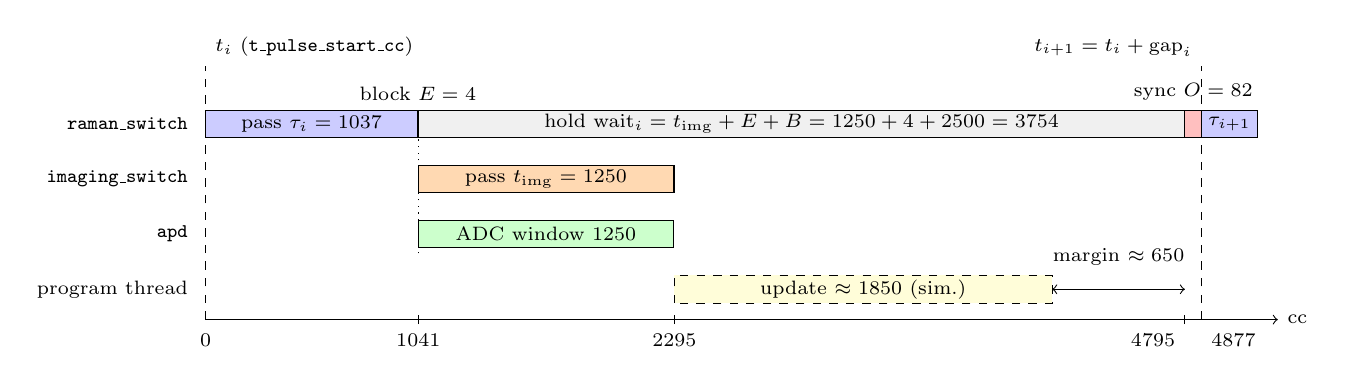
\begin{tikzpicture}[x=0.0026cm, y=0.7cm, font=\scriptsize]
  % row labels
  \node[anchor=east] at (-40,3.25) {\code{raman\_switch}};
  \node[anchor=east] at (-40,2.25) {\code{imaging\_switch}};
  \node[anchor=east] at (-40,1.25) {\code{apd}};
  \node[anchor=east] at (-40,0.25) {program thread};
  % pulse starts
  \draw[dashed] (0,-0.3) -- (0,4.3);
  \draw[dashed] (4877,-0.3) -- (4877,4.3);
  \node[anchor=south west] at (0,4.3) {$t_i$ (\code{t\_pulse\_start\_cc})};
  \node[anchor=south east] at (4877,4.3) {$t_{i+1} = t_i + \mathrm{gap}_i$};
  % raman_switch
  \draw[fill=blue!20] (0,3.0) rectangle (1037,3.5);
  \node at (518,3.25) {pass $\tau_i = 1037$};
  \draw[fill=black] (1037,3.0) rectangle (1041,3.5);
  \node[anchor=south] at (1039,3.5) {block $E = 4$};
  \draw[fill=gray!12] (1041,3.0) rectangle (4795,3.5);
  \node at (2918,3.25) {hold $\mathrm{wait}_i = t_{\rm img} + E + B = 1250 + 4 + 2500 = 3754$};
  \draw[fill=red!25] (4795,3.0) rectangle (4877,3.5);
  \node[anchor=south] at (4836,3.5) {sync $O = 82$};
  \draw[fill=blue!20] (4877,3.0) rectangle (5150,3.5);
  \node at (5013,3.25) {$\tau_{i+1}$};
  % imaging_switch
  \draw[dotted] (1041,0.9) -- (1041,3.0);
  \draw[fill=orange!30] (1041,2.0) rectangle (2291,2.5);
  \node at (1666,2.25) {pass $t_{\rm img} = 1250$};
  \draw[fill=black] (2291,2.0) rectangle (2295,2.5);
  % apd
  \draw[fill=green!20] (1041,1.0) rectangle (2291,1.5);
  \node at (1666,1.25) {ADC window 1250};
  % program thread
  \draw[dashed, fill=yellow!15] (2295,0.0) rectangle (4145,0.5);
  \node at (3220,0.25) {update $\approx 1850$ (sim.)};
  \draw[<->] (4145,0.25) -- (4795,0.25);
  \node[anchor=south] at (4470,0.5) {margin $\approx 650$};
  % axis
  \draw[->] (0,-0.3) -- (5250,-0.3);
  \node[anchor=west] at (5250,-0.3) {cc};
  \draw (1041,-0.38) -- (1041,-0.22);
  \draw (2295,-0.38) -- (2295,-0.22);
  \draw (4795,-0.38) -- (4795,-0.22);
  \node[anchor=north] at (0,-0.38) {0};
  \node[anchor=north] at (1041,-0.38) {1041};
  \node[anchor=north] at (2295,-0.38) {2295};
  \node[anchor=north east] at (4795,-0.38) {4795};
  \node[anchor=north west] at (4877,-0.38) {4877};
\end{tikzpicture}
\caption{One feedback cycle as scheduled, in 4\nsu\ clock cycles, for the
first drawn pulse of the simulated shot ($\tau_0 = 1037$\,cc $= 4.15\us$) and
the default parameters ($t_{\rm img} = 1250$, $B = 2500$, $O = 82$, $X = 0$):
$\mathrm{gap}_i = \tau_i + 3840$\,cc. The exposure and the ADC window are drawn
starting at the Raman block's end; the aligns delay them by a few cycles (in
the first-pass structure the exposure started 9\,cc after the Raman pass
ended: the 4-cc block plus 5\,cc of sync), inside the hold, without moving
$t_{i+1}$. The program-thread row is the simulator's per-pulse compute for the
default structure (1938\,cc including the 82-cc sync,
section~\ref{sec:feedback:speed}), placed after the exposure; it is a
measured duration, not a timestamp. The next pulse's IF update, phase reset
and align are the sync $O$.}
\label{fig:feedback:cycle}
\end{figure}

With the default numbers a cycle is $\tau_i + 3840$\,cc $= 18.9$--$22.5\us$
for $\tau_i = 890$--$1780$\,cc ($0.5$--$1.0\,t_\pi$), against ARTIQ's
57--61\us\ (section~\ref{sec:why}).

\paragraph{Why the overhead must be exact.} The OPX's real-time posterior
uses the \emph{scheduled} starts: the frame advance of hypothesis $j$ over
step $i$ is $\operatorname{frac}(f_j\,\mathrm{gap}_i)$
(section~\ref{sec:feedback:numerics}). If the true constant $O$ differs from
the parameter by one cycle, every hypothesis's phase is wrong by 0.478 turns
per step, and the error accumulates. The simulator shows it: with the
previous structure's value (91\,cc) on the pass-3b loop, the pulse starts
drifted by $-9$\,cc per interval ($0, -9, -18, \dots, -45$ over six pulses),
i.e.\ $9 \times 0.478 = 4.3$ turns per step; with 82\,cc (and 86\,cc for the
discrete-duration structure) the simulated slip is 0 on every pulse. The
replay, which uses the timestamps, is unaffected either way.

\subsection{The exact applied frequency}
\label{sec:feedback:freq}

The drive of every pulse is a \emph{grid index} $d$: the control law picks the
argmax, and the initial drive is snapped to the grid point nearest
\code{feedback\_fractional\_initial\_offset} (the grid is built around the
rounded offset, so with the default grid -- offset 0, span 5 -- the snap is
the identity; with the \code{feedback\_opx.py} config -- offset 2, span 3 --
the grid snap onto resonance moves it $2.0 \to 2.1$, at most half a step in
general). For every grid point the host computes the two integer IFs once per
run from the Raman split,
\[
  \mathrm{IF}_{el}[j] = \mathrm{IF0}_{el} + \operatorname{round}\big(s_{el}\, w_j\, f_\Omega\big),\qquad
  s_{80} = -\tfrac{8}{46},\quad s_{150} = +\tfrac{15}{46},\quad f_\Omega = \frac{1}{2t_\pi},
\]
with \code{IF0} and the slopes from \code{ctx.transition\_offset\_terms('raman')}
(the \code{RamanBeamPair} split, numerically differentiated at trace time), and
the OPX applies \code{if80T[d]}, \code{if150T[d]} with
\code{ctx.set\_frequency(..., which=)}. The two-photon frequency the atoms see
is, for the $+1/{+1}$ double-pass pair,
\[
  f_{\rm applied}[d] = 2\,\big(\mathrm{IF}_{150}[d] - \mathrm{IF}_{80}[d]\big),
\]
asserted at trace time to reproduce \code{frequency\_raman\_transition} from
the \code{IF0}s within 3\,Hz (and $2(s_{150} - s_{80}) = 1$ to $10^{-9}$). The
sequence streams $d$ per pulse (\code{drive\_index}) and records the integer
table (\code{if\_table\_hz}, shape $(m, 2)$), so the finish hook and the replay
know the applied frequency \emph{exactly}; every grid point is within 3\,Hz
($4\times 10^{-5}\,\Omega$) of $f_0 + w_j f_\Omega$
(\code{test\_if\_tables\_invert\_to\_the\_two\_photon\_frequency}). The QM
documentation gives no finite NCO quantum (``sub-Hz resolution'';
\code{update\_frequency} takes integer Hz ``in steps of 1''), so the integer
Hz commanded is taken as the applied frequency.

\subsection{The per-pulse algorithm on the OPX}
\label{sec:feedback:numerics}

QUA \code{fixed} is 4.28: range $[-8, 8)$, wrap modulo 16, and the
\code{Math} library has domain limits. Everything is therefore rescaled.
Frequencies are in units of $\Omega = \pi/t_\pi$, $w = (\omega - \omega_0)/\Omega$;
the grid is descending, $w_j = w_0 - j\,\Delta w$ ($\Delta w = 2\,\mathrm{span}/(m-1)$:
0.3 for span 3, 0.5 for span 5), with $w_{\rm zidx} = 0$ exactly. Rotation
angles are in turns.

\paragraph{Axis geometry from tables (idea A).} With the drive at index $d$,
the drive--hypothesis detuning is $\delta_j = w_d - w_j = (j - d)\,\Delta w$ and
depends only on $k = j - d \in [-(m-1), m-1]$. Five run tables of length
$2m - 1 = 41$, indexed by $j + (m - 1 - d)$, replace the per-point
\code{Math.inv\_sqrt}:
\[
  h_k = \sqrt{\tfrac{1}{16} + \big(\tfrac{k\,\Delta w}{4}\big)^2} = \frac{|H_k|}{4\Omega},\qquad
  u_{x,k} = \frac{\Omega}{|H_k|} = \frac{1}{4h_k},\qquad
  u_{z,k} = \frac{\delta}{|H_k|} = \frac{k\,\Delta w/4}{h_k},
\]
plus $u_{x,k}^2$ and $u_{x,k}u_{z,k}$. The tables refuse $(m-1)\Delta w > 10.9$
(so $h^2 < 8$).

\paragraph{Rotation angle and the sine table.} With $a_i = (\tau_i -
t_{\rm off})/(2t_\pi)$ (shipped as $-4a_i$, \code{theta\_scale\_x4}), the pulse
angle is $\theta_{i,k} = -4a_i\,h_k$ turns (the model's $-|H|\,\tau_{\rm ideal}$).
Its cosine and sine come from a table $T[n] = \sin(2\pi n/N)$, $N = 2^{12}$,
$n = 0, \dots, N + N/4 + 1$ (5122 entries), read from the 4.28 bit pattern
$u$ of $\theta$: $r = u \bmod 2^{28}$ (the fraction of a turn; negative angles
wrap correctly), $n = \lfloor r/2^{16}\rfloor$, $\varphi = (r \bmod 2^{16})/2^{16}$,
\[
  \sin 2\pi\theta \approx T[n] + \varphi\,(T[n+1] - T[n]),\qquad
  \cos 2\pi\theta \approx T[n + \tfrac N4] + \varphi\,(T[n + \tfrac N4 + 1] - T[n + \tfrac N4]),
\]
error $\le (2\pi/N)^2/8 = 2.9\times 10^{-7}$ on the trig values
(\code{opx\_sincos\_lut\_bits = 12}; 0 selects \code{Math.cos2pi}/\code{sin2pi}, exact).

\paragraph{Co-rotating azimuth frame with one merged $z$-rotation (idea D).}
The rotation axis of hypothesis $j$ at pulse $i$ is $\hat u = R_z(\phi_{j,i})\,\hat
u_0$ with $\hat u_0 = (u_x, 0, u_z)$, so $R(\hat u, \theta) = R_z(\phi)\,R(\hat u_0,
\theta)\,R_z(-\phi)$. The OPX keeps each hypothesis in the frame where its
next axis lies in the $x$--$z$ plane, $\tilde s_{j,i} = R_z(-\phi_{j,i})\,s_{j,i}$.
Then, with $c = \cos 2\pi\theta$, $s = \sin 2\pi\theta$ and $u_y = 0$, the Rodrigues
rotation has five distinct entries,
\[
  R(\hat u_0, \theta) =
  \begin{pmatrix} A & -B & K \\ B & c & -D \\ K & D & E \end{pmatrix},\quad
  A = c + (1-c)u_x^2,\ B = s\,u_z,\ K = (1-c)\,u_xu_z,\ D = s\,u_x,\ E = 1 - (1-c)u_x^2,
\]
and the whole step is
\[
  \tilde s_{j,i+1} = C_{xy}\,R_z(\gamma_{j,i})\,R(\hat u_0, \theta_{i,k})\,\tilde s_{j,i},\qquad
  \gamma_{j,i} = \phi_{j,i} - \phi_{j,i+1} - \alpha_{j,i},
\]
where $\alpha_{j,i} = b_i(w_j - w_d) - \phi_{LS}$ (turns, $b_i = \tau_i/(2t_\pi)$) is
\code{generate\_posterior}'s light-shift and drive-frame return, and $C_{xy}$
multiplies $x, y$ by $C$. The frame change and the $z$-rotation have merged
into one angle, and $\gamma$ is linear in $j$:
\begin{align*}
  \gamma_{j,i} &= \big(\Delta\phi_{0,i} + \beta_i\big) + j\,\big(\Delta\mathrm{d}\phi_i + \Delta\beta_i\big),\\
  \beta_i &= 4b_i\Big(\frac{w_d}{4} - \frac{w_0}{4}\Big) + \phi_{LS},\qquad \Delta\beta_i = 4b_i\,\frac{\Delta w}{4},\\
  \Delta\phi_{0,i} &= \operatorname{frac}\big(f_0\,(t_{i+1} - t_i)\big),\qquad
  \Delta\mathrm{d}\phi_i = \operatorname{frac}\big((f_1 - f_0)\,(t_{i+1} - t_i)\big).
\end{align*}
The frame advances depend only on the scheduled step $\mathrm{gap}_i$; the
host ships their cosines and sines (\code{cos\_dphi0}, \code{sin\_dphi0},
\code{cos\_ddphi}, \code{sin\_ddphi}) over an $(N{+}1)$-row schedule whose last
row is a would-be pulse $N$ (\code{corotating\_phase\_tables},
\code{extend\_schedule\_cc}). Per pulse the OPX forms $\cos,\sin$ of $\beta_i$
and $\Delta\beta_i$ (four trig calls) and the seed and step phasors
\[
  (c_\gamma, s_\gamma) = C\,\big(\cos 2\pi\gamma_{0,i},\ \sin 2\pi\gamma_{0,i}\big),\qquad
  (c_\Delta, s_\Delta) = \big(\cos 2\pi\Delta\gamma_i,\ \sin 2\pi\Delta\gamma_i\big)
\]
by angle addition, with $C$ folded into the seed; per grid point it applies
$x \leftarrow c_\gamma x' - s_\gamma y'$, $y \leftarrow s_\gamma x' + c_\gamma y'$, $z
\leftarrow z'$ and steps $(c_\gamma, s_\gamma)$ by $(c_\Delta, s_\Delta)$ -- one phasor
recurrence per point instead of two, a 5-entry mat-vec instead of the full
Rodrigues (23 multiplies and 13 adds instead of 49 and 22 as emitted). $z$,
$s_z$ and the likelihood are identical to the lab frame (verified to
$10^{-12}$ against the previous form); $x, y$ are the same vector in a
different frame. The spin-up initial state is frame-invariant.

\paragraph{The measurement.} \code{ctx.measure} returns the raw integration
result $v$ ($\mathrm{raw} = V \times \mathrm{duration\_ns}/4096$). With the
endpoints $v_{\rm up,raw}$, $v_{\rm down,raw}$ converted from the OPX volts
parameters and $r = 1/(v_{\rm up,raw} - v_{\rm down,raw})$ split as $r = k_1 n$
with the smallest $n \in \{1, 2, 4, 8\}$ giving $|k_1| < 8$ ($n = 2$ for the
placeholder calibration, $r = 11.2$):
\[
  p_{\rm meas} = \Big(\operatorname{clamp}\big((v - v_{\rm down,raw})\,k_1,\ [-2, 3]/n\big)\Big) \times 2 \times \cdots\ (\log_2 n\ \text{doublings}),
\]
i.e.\ the photon fraction clamped \emph{once per pulse} to $[-2, 3]$ -- a bound
that is never reached at nominal noise and that caps $|p_{\rm meas} - p_1| \le 3$.

\paragraph{The likelihood as $L/32$ (ideas F, F').} The OPX keeps the log
weights as $\ell_j = L_j/s$ with $s$ = \code{feedback\_log\_weight\_scale} $= 32$.
Since $p_1$ is monotonic with $p_1(\pm 1) \in \{0, 1\}$ (asserted:
$m_f \in (0.25, 0.75)$), neither $p_1$ nor the residual needs a clamp:
\[
  p_1 = \tfrac12(1 + z') + (m_f - \tfrac12)(1 - z'^2),\qquad
  q = \frac{p_{\rm meas} - p_1}{\sigma_p\sqrt{2s}} = \frac{p_{\rm meas} - p_1}{8\,\sigma_p},\qquad
  \frac{\Delta L}{s} = -q^2 \in [-5.55,\ 0].
\]
This is the ARTIQ Gaussian exactly: $\Delta L = -(p_{\rm meas} - p_1)^2/(2\sigma_p^2)$.
The max-normalisation is \emph{lazy}: pulse $i$'s loop reads the previous
pulse's maximum $M_{i-1}$ (0 at shot start) and does, per point,
\[
  \ell_j \leftarrow \max\big(\ell_j - M_{i-1},\ F\big) - q_j^2,\qquad
  F = -8 + \Big(\frac{3}{\sigma_p\sqrt{2s}}\Big)^2 + 2^{-16} = -2.452\quad (sF = -78.5\ \text{nats}),
\]
one \code{Util.cond} and one multiply, so $\ell \in [-8, 0]$ by construction;
then $j_{\max}$ = \code{Math.argmax}$(\ell)$, $M_i = \ell_{j_{\max}}$, and the saves
emit $\ell_j - M_i \in [-8, 0]$. The floor is derived from $\sigma_p$ and the
$p_{\rm meas}$ bound, not a free parameter. The host recovers the posterior as
$P_j = e^{s(\ell_j - M_i)}/\sum_k e^{s(\ell_k - M_i)}$.

\paragraph{The control law (idea G).} The next drive is $d \leftarrow j_{\max}$
(\code{feedback\_flat\_rule\_bool = 0}). ARTIQ's flat rule (drive the posterior
mean when $\max P < 1.15/m$) never fired in 6000 synthetic pulses of any
model-consistent scenario: the flattest posterior, after the first pulse,
has $m \max P \ge 1.18$ against the 1.15 threshold (drive parked at the grid
edge), and the rule fires only when readings are $\ge 3\times$ noisier than
the model. Dropping it removes the whole exp/sum/inv/dot pass. With the flag
at 1 the ARTIQ rule is restored: $\ell_j \leftarrow \ell_j - M$, $e^{\ell}$ from a
2050-entry interpolation table (\code{opx\_exp\_lut\_bits} $= 8$; 0 =
\code{Math.exp}) followed by $\log_2 s = 5$ squarings, weights kept as $P/4$
(sum in $[\tfrac14, \tfrac m4]$, $m \le 31$ asserted), flat iff $\sum P/4 >
m/4.6$, and the mean $4\,\mathrm{dot}(P/4, w/4)/\sum(P/4)$ \emph{snapped to the
nearest grid index} (\code{Math.argmin}), because the drive is an index. The
flat-rule structure has not been timed.

\paragraph{Discrete pulse durations (ideas B + E, option).} With
\code{t\_raman\_pulse\_n\_levels} $= n \ge 4$ every duration is drawn
uniformly from $n$ levels equally spaced on $[0.5, 1.0]\,t_\pi$ (each on the
4\nsu\ grid; \code{draw\_t\_raman\_pulse\_list\_levels}, a pure function of the
seed). The five matrix entries per $(l, k)$ ($n(2m-1)$ values each), the seed
phasors per $(l, d)$ and the step phasors per $l$ are then run tables and the
real-time loop has \emph{no trig at all}; $E = (1 + c) - A$. Physics: 2 and 3
levels alias measurably ($+5$--7\,\% wrong-grid-point rate, $3\sigma$); 4--16
levels sit within $+0.6$..$+3$\,\% of the continuous draw at 1000 seeds
($\le 2\sigma$). Fewer than 4 levels are refused, $\ge 8$ (better 16) are
recommended, and a 10k-seed comparison is owed before the option is used.
Default 0 = continuous.

\paragraph{What differs from the ARTIQ posterior.} The posterior itself has
three approximations left: the $-78.5$\,nat floor (hit in $\sim 0.4$\,\% of
hypothesis updates at nominal noise in the synthetic study), the sine table,
and QUA's $2^{-28}$ rounding of every product (not modelled by the
emulation; it flips about 1\,\% of argmax decisions at near-ties). The
$p_{\rm meas}$ clamp never fires at nominal noise. The control differs by the
two rules above: argmax only, and a grid-snapped initial drive. ARTIQ's
degenerate branch (``every weight underflowed to zero $\to$ reset to uniform'')
cannot occur with max-normalised log weights. Against the unclamped
double-precision posterior the $L/32$ scheme agrees to $8\times 10^{-34}$ at
nominal noise and $2\times 10^{-8}$ at $4\times$ noise, where the previous $L/4$
representation with a $7.9\sigma$ residual clamp changed 32\,\% of the argmax
decisions -- so the change is a fidelity fix as well as a speed-up.
\code{test\_numerics\_oracle\_matches\_generate\_posterior} requires, over 6
seeds $\times$ 20 pulses, $P$ within $10^{-6}$ and identical decisions (exact
ties aside) with exact trig, and with the sine table $P$ within
$5\times 10^{-5}$ (measured $\le 5\times 10^{-7}$), $s_z$ within $10^{-6}$ and
identical decisions.

\paragraph{What the sequence refuses at trace time.} Remesh
(\code{feedback\_remesh\_threshold\_Omega} $\ne 0$; section~\ref{sec:feedback:remesh});
\code{feedback\_phase\_model\_reset} $\ne 1$; \code{t\_raman\_pulse\_block\_bool}
$\ne 0$; \code{update\_raman\_frequency\_bool} disagreeing with the mode (1
closed loop, 0 open loop, so the run file says what ran); \code{t\_img\_pulse}
$\ne$ \code{t\_imaging\_pulse\_apd\_abs} (the exposure and the ADC window are
one and the same); a transition that varies per shot; a Raman split that is
not the $+1/{+1}$ double pass; $m > 31$; $\sigma_p \le 0.125$; a log-weight
scale that is not a power of two or leaves no room under the floor; a
midpoint outside $(0.25, 0.75)$ with the remap on; sine-table bits outside
$\{0\} \cup [4, 14]$, exp-table bits outside $[0, 10]$; 1--3 duration levels, or
levels with a scanned span or duration range; a drawn pulse or a hold under
4\,cc; $(m-1)\Delta w > 10.9$; grid values $\ge 8$; rotation or seed angles out of
the fixed range; an overhead or extra gap that is not a non-negative multiple
of 4\nsu; a budget under 16\nsu; the flat rule with a per-shot grid; APD
endpoints outside the fixed range in raw units, or so close that
$1/(v_{\rm up,raw} - v_{\rm down,raw}) \ge 64$.

\subsection{Speed: what the simulator measured}
\label{sec:feedback:speed}

All numbers are from the QOP simulator (2026-09-25) through \code{OPXBench};
none is from hardware. \textbf{Statement costs} were measured with
one-statement loop bodies bracketed by timestamped plays, per-iteration cost
$= (\mathrm{lat}(42) - \mathrm{lat}(21))/21$. Bodies cheaper than $\sim$10\,cc
(empty, array read/write, add, mul, cond, expression index) came back
inconsistent or negative -- when the loop is shorter than the play pipeline
the second bracket play is issued as soon as the element is free -- so only
the compute-bound rows are quoted:

\begin{table}[htbp]
\centering\small
\begin{tabular}{@{}lr@{}}
\toprule
loop body (per iteration) & cc \\
\midrule
\code{Math.cos2pi} & 21.4 \\
\code{Math.cos2pi} + \code{Math.sin2pi} & 27.7 \\
\code{Math.inv\_sqrt} & 64.3 \\
\code{Math.exp} & 60.2 \\
exp interpolation block (5 statements) & 16.1 \\
sine-table block (6 statements; 1024 or 4096 nodes alike) & 24.2 \\
\code{Math.argmax} over 64 entries & 224.7 \\
mat-vec (5-entry matrix + $z$-rotation) & 22.3 \\
pass-2 Rodrigues rotation, as emitted & 35.9 \\
new per-point body, \code{Math} trig (3 axis tables) & 82.0 \\
new per-point body, sine table & 75.0 \\
new per-point body, 5 axis tables, \code{Math} trig & 77.0 \\
new per-point body, $(l, k)$ tables (no trig) & 32.7 \\
\bottomrule
\end{tabular}
\caption{QUA statement costs on the QOP simulator (module docstring of
\file{opx\_sequences/feedback.py}). Adopted: the sine table (12 bits), the
5 axis tables, and the $(l, k)$ tables as an option.}
\label{tab:feedback:stmt}
\end{table}

\textbf{Per-pulse compute} is the excess of each pulse-to-pulse interval over
$\tau_i + E + t_{\rm img} + E$ with the budget collapsed to 16\nsu, i.e.\ the
readback, the update and the sync after the exposure ($m = 21$, $N = 6$, a DC
level on the APD input so the weights are nontrivial). It was identical on
every one of the five intervals of each run:

\begin{table}[htbp]
\centering\small
\begin{tabular}{@{}lrr@{}}
\toprule
structure & cc & \micro s \\
\midrule
pass 2: fused loop, \code{inv\_sqrt}, exp table, flat rule & 4875 & 19.50 \\
pass 3b, continuous durations, exact trig & 2043 & 8.17 \\
\textbf{pass 3b, continuous durations, 12-bit sine table (default)} & \textbf{1938} & \textbf{7.75} \\
pass 3b, 16 discrete durations ($(l, k)$ tables) & 1074 & 4.30 \\
\bottomrule
\end{tabular}
\caption{Per-pulse compute after the imaging exposure (simulator,
2026-09-25). The first pass (2026-09-24) needed 25.7\us. Exact trig and the
sine table gave identical decisions.}
\label{tab:feedback:perpulse}
\end{table}

\paragraph{Budget and overhead.} \code{t\_opx\_feedback\_compute\_budget} $=
10\us$ (2500\,cc): the default structure needs $\sim$1850\,cc beyond the
scheduled hold and exact trig $\sim$1955\,cc, a 35\,\% / 28\,\% margin for
hardware versus simulator. With it every simulated interval equals the
schedule plus a constant sync of 82\,cc (continuous) or 86\,cc (discrete
levels), carried by two parameters, and with them the simulated slip is 0 on
every pulse. The flat-rule structure has not been timed; expect the slip line
to fire until it is.

\paragraph{What did not work, and why.}
\begin{itemize}[nosep]
  \item \textbf{Overlapping the prediction with the pulse or the exposure.}
    Issuing the Bloch prediction (everything but the likelihood) after the
    play/measure statements gave 26.3\us\ against 25.3\us\ fused; before the
    play, 26.7\us, and it delayed the pulse by the loop length. Classical
    statements run in the program thread's order with the pulse stream, and
    \code{measure} blocks the thread until its result exists. Deferring the
    log-weight saves gained nothing.
  \item \textbf{Unrolling} the grid loop in Python did not compile within
    120\,s.
  \item \textbf{Multi-core parallelism} (assessed, refuted for this workload
    on QOP 2.6). The OPX+ has one core per element with a hardware sync path,
    and the QM guides speak of loops ``supposed to run in parallel''. A
    simulator probe split the 21 hypotheses into $K$ disjoint blocks, each
    with its own iterator and state and each bound to a spare digital element
    by a per-iteration \code{wait} or 16-ns play; the body was a standalone
    copy of the pass-2 update, so the absolute numbers are not those of the
    table above. Measured per-pulse update:
    one block 5290\,cc; $K = 2$: 5409 ($+2.2$\,\%); $K = 3$: 5476 ($+3.5$\,\%);
    $K = 4$: 5688 ($+7.5$\,\%); the same-core control ($K = 2$ with every block
    element on one core) 5409, indistinguishable from the ``parallel'' split.
    The per-iteration ticks of all blocks were issued within the first
    $\sim$0.8\us\ of a $\sim$21\us\ window: they are queued to the pulsers up
    front, so interleaved ticks say nothing about where the arithmetic ran.
    The compiler emits all classical statements as one sequential stream,
    whatever element a loop is bound to. A hardware timestamp check would
    confirm it; nothing suggests trying further.
  \item \textbf{Stream-processing offload} is impossible: stream processing
    is one-way (OPX $\to$ server); the only return paths (input streams, IO
    variables with \code{pause}) have millisecond latency and cannot be
    simulated.
  \item \textbf{Angle-addition stepping of $\cos\theta, \sin\theta$ across $j$}:
    refuted, $\theta_k \propto h_k$ is not linear in $k$; only the discrete
    durations turn it into a table.
\end{itemize}

\subsection{Per-shot host work, and the data it saves}
\label{sec:feedback:data}

At trace time \code{build\_feedback\_shot\_tables} reads the columns (the seed
-- 0 draws a fresh seed per shot with \code{new\_t\_raman\_pulse\_seed(0)} --,
\code{t\_raman\_pulse\_random\_bool}, the min/max fractions,
\code{feedback\_fractional\_initial\_offset} and \code{feedback\_guess\_span\_Omega},
both of which may be scanned) and the run constants (\code{feedback\_constants}
via \code{ctx.const}); draws $\tau_{\rm cc}[\mathrm{shot}, i]$ with the same
\code{draw\_t\_raman\_pulse\_list} as ARTIQ (or the level draw), rounded to
4\nsu\ cycles; and builds per shot the gaps, holds and $(N{+}1)$-row schedule,
the grid, $a_i$, $b_i$, the frame-advance tables, the integer IF tables and,
per run, the axis or $(l, k)$ tables. Tables constant over the run become
plain QUA arrays declared with their values; per-shot ones become shot arrays
(\code{t\_raman\_pulse\_cc}, \code{t\_wait\_cc}, \code{theta\_scale\_x4},
\code{alpha\_scale\_x4}, \code{cos/sin\_dphi0}, \code{cos/sin\_ddphi};
\code{level\_idx} with discrete durations; the IF, axis, \code{zidx} and
initial-drive tables only when the grid is scanned;
\code{drive\_schedule\_idx} open loop). Per-shot QUA state: $x, y, z, \ell$
($m$ each), $M$, $d$ and about 40 scalars.

The saved data are only what the replay needs, plus the one thing the reset
model cannot reconstruct (the actual pulse starts):

\begin{center}\small
\begin{tabular}{@{}llp{7.6cm}@{}}
\toprule
key & per-shot shape & meaning \\
\midrule
\multicolumn{3}{@{}l}{\emph{streams (from the OPX)}} \\
\code{apd} & $(N)$ float & the APD integration per pulse; raw on the OPX, \textbf{stored as volts} (\code{demod2volts}, like every \code{ctx.measure} key) \\
\code{drive\_index} & $(N)$ int & the grid index driven at pulse $i$ (pulse 0: the snapped initial drive); $-1$ where missing \\
\code{s\_z} & $(N)$ float & $z_{\rm zidx}$ after update $i$ (the model's $S_z$ under the on-resonance hypothesis, as on ARTIQ) \\
\code{log\_weights} & $(N, m)$ float & $\ell_j - M_i = L/s$ after the max-normalisation, $s$ = \code{feedback\_log\_weight\_scale} \\
\code{t\_pulse\_start\_cc} & $(N)$ int & timestamp of each Raman \code{'pass'} play, cycles from program start \\
\code{opx\_shot\_index}, \code{opx\_data\_valid} & $(1)$ int & echo and mask (framework) \\
\multicolumn{3}{@{}l}{\emph{host data (recorded at trace time)}} \\
\code{t\_raman\_pulse}, \code{t\_raman\_pulse\_seed} & $(N)$, $(1)$ & the drawn durations on the 4\nsu\ grid (what ran) and the seed \\
\code{omega\_raman\_mesh} & $(N{+}1, m)$ & the grid (rad/s), every row equal \\
\code{if\_table\_hz} & $(m, 2)$ & integer IFs \code{[raman\_80, raman\_150]} of every grid point (Hz; integer values in a float64 container) \\
\multicolumn{3}{@{}l}{\emph{derived by the finish hook (declared as host data, NaN until then)}} \\
\code{omega\_raman} & $(N)$ & $2\pi \cdot 2\,(\mathrm{IF}_{150}[d] - \mathrm{IF}_{80}[d])$, rad/s: the exact applied drive \\
\code{probabilities} & $(N{+}1, m)$ & row 0 uniform, rows $1..N$ = $e^{s\ell}/\sum e^{s\ell}$ \\
\code{t\_pulse\_start} & $(N)$ & actual pulse starts, s from pulse 0 (differences mod $2^{32}$; placeholders $< 0$ and invalid shots $\to$ NaN) \\
\code{t} & $(N)$ & $t_{\rm start} + \tau_i + t_{\rm img}$: end of imaging, the ARTIQ convention for plots \\
\bottomrule
\end{tabular}
\end{center}

Everything else -- the schedule, the gaps and holds, the frame tables, the
axis tables, the open-loop drive schedule -- is a pure function of these and
the params and is recomputed where needed (\code{feedback\_finish},
\code{FeedbackOPXReplay}). There is no slip container: the finish hook
recomputes the schedule (\code{scheduled\_pulse\_starts\_s}) and prints
\code{[opx feedback] slip: <max> cycles max |slip| over <n> shots}, plus a
\code{***} line when any pulse is more than half a cycle off it; the replay
returns the slip per pulse. The ARTIQ names (\code{apd}, \code{omega\_raman},
\code{s\_z}, \code{t}, \code{probabilities}, \code{omega\_raman\_mesh},
\code{t\_raman\_pulse}, \code{t\_raman\_pulse\_seed}) are kept so the existing
analysis conventions carry over. Files from the previous pass
(\code{log\_weights4} $= L/4$, \code{dif\_hz}) are still read by the finish
hook and the replay.

\paragraph{Reading a feedback run back.}

\begin{lstlisting}[style=py]
import numpy as np
from kexp import atomdata
from kexp.experiments.opx_sequences.feedback import (
    applied_frequency_hz, log_weights_to_probabilities, scheduled_pulse_starts_s)

ad = atomdata(run_id, roi_id='auto')
N, m = int(ad.p.N_pulses), int(ad.p.feedback_grid_size)
s = float(ad.p.feedback_log_weight_scale)             # 32: log_weights = L/s
valid = ad.data.opx_data_valid.reshape(-1).astype(bool)   # 1 = the OPX ran this shot

apd   = ad.data.apd.reshape(-1, N)                    # volts (demod2volts); NaN where not valid
d_idx = ad.data.drive_index.reshape(-1, N)            # grid index driven; -1 where missing
ift   = ad.data.if_table_hz.reshape(-1, m, 2)         # integer IFs [raman_80, raman_150], Hz
omega = ad.data.omega_raman.reshape(-1, N)            # rad/s, 2 pi * 2 (if150[d] - if80[d])
P     = ad.data.probabilities.reshape(-1, N + 1, m)   # row 0 uniform, row i+1 after pulse i
L     = ad.data.log_weights.reshape(-1, N, m)         # what the OPX saved (L/s, max-normalised)
t0    = ad.data.t_pulse_start.reshape(-1, N)          # actual pulse starts, s from pulse 0
tau   = ad.data.t_raman_pulse.reshape(-1, N)          # drawn durations, 4 ns grid
mesh  = ad.data.omega_raman_mesh.reshape(-1, N + 1, m)

f_app = applied_frequency_hz(ift, d_idx)              # Hz; equals omega / 2 pi
P_chk = log_weights_to_probabilities(L, s)            # what the finish hook wrote into P[:, 1:]
slip  = t0 - scheduled_pulse_starts_s(ad.p, tau)      # s; 0 when the OPX kept the schedule
print(np.nanmax(np.abs(slip[valid])) / 4e-9, 'cycles of worst slip')

Omega = np.pi / ad.p.t_raman_pi_pulse
w = (mesh[:, 1:, :] - 2 * np.pi * ad.p.frequency_raman_transition) / Omega
w_mean = np.sum(P[:, 1:, :] * w, axis=-1)             # posterior mean per pulse, Omega units
\end{lstlisting}

\subsection{The experiment files}

\code{feedback\_opx.py} (\code{class feedback\_opx(EnvExperiment, Base)}) is
\code{feedback\_fast.py} with the loop moved: \code{Base.\_\_init\_\_(camera\_select=
cameras.apd, imaging\_type=img\_types.DISPERSIVE, expt\_params=ExptParamsFeedbackOPX(),
save\_data=True, save\_on\_underflow=True)}; \code{update\_raman\_frequency\_bool = 1},
\code{feedback\_fractional\_initial\_offset = 2}, \code{N\_repeats = 21},
\code{N\_pulses = 17}, \code{feedback\_guess\_span\_Omega = 3};
\code{self.opx.use(bayesian\_feedback)}; \code{finish\_prepare(shuffle=True)}.
\code{feedback\_opx\_deterministic.py} is the open-loop grid sweep
(\code{deterministic\_bayesian.py} on the OPX): \code{update\_raman\_frequency\_bool
= 0}, \code{N\_pulses = 9}, grid 21 with half-width 2, the drive of pulse $i$
at grid index \code{rint(linspace(0, m-1, N))[i]} (\code{open\_loop\_drive\_indices})
while the posterior still runs and is saved; scanning the initial offset
slides where the resonance sits in the prior. Both \code{scan\_kernel}s:
\code{set\_imaging\_detuning(midpoint)}, \code{imaging.set\_power},
\code{prepare\_hf\_tweezers(squeeze=True)},
\code{prep\_raman(frequency\_transition=p.frequency\_raman\_transition,
phase\_mode=0)}, handoff, hand-back, \code{delay(t\_tweezer\_hold)},
\code{raman\_shutter.off}, \code{tweezer.off}, \code{delay(t\_tof)},
\code{abs\_image()}. The ARTIQ \code{Integrator}, the Sampler read, the AD9910
fast-frequency-update machinery and the kernel posterior all disappear from
the shot. The header docstrings say NOT YET RUN ON HARDWARE and list M1--M3.

\subsection{The replay class}
\label{sec:feedback:replay}

\code{FeedbackOPXReplay(ad, use\_actual\_timestamps=True, lut\_size=2**20)}
in \file{kexp/analysis/feedback\_opx.py} subclasses \code{Feedback} and
reuses \code{generate\_posterior} exactly:

\begin{lstlisting}[style=py]
from kexp import atomdata
from kexp.analysis import FeedbackOPXReplay

ad = atomdata(run_id, roi_id='auto')
fr = FeedbackOPXReplay(ad)              # actual pulse timestamps by default
res = fr.replay_measured()              # double precision, phase 0, the exact applied drive
out = fr.compare_with_opx(res)          # |dP|, argmax agreement (>= 99 % expected), worst slip
res_fp = fr.emulate_fixed_point(True).replay_measured()   # the OPX algorithm in float64
fr.emulate_fixed_point(False)
fr.p.frequency_lightshift = 45.e3       # what-if on a model constant
res_cf = fr.simulate_counterfactual()   # the replay picks its own drives
synth = fr.simulate_feedback_run_apd(detuning_offset_Omega=0.37, seed=1)
\end{lstlisting}

\begin{itemize}[nosep]
  \item \textbf{Inputs.} \code{apd} and \code{t\_raman\_pulse} (required);
    the drive from \code{drive\_index} + \code{if\_table\_hz} (older files:
    \code{dif\_hz}, then \code{omega\_raman}); \code{s\_z}; \code{log\_weights}
    with the saved scale (or \code{log\_weights4}, or \code{probabilities});
    the seed; \code{t\_pulse\_start} (or the raw \code{t\_pulse\_start\_cc});
    \code{omega\_raman\_mesh}; \code{opx\_data\_valid}. Per-shot columns of a
    scanned offset or span are honoured.
  \item \textbf{Calibration mapping.} \code{fr.p} is a copy of \code{ad.p} with
    the OPX calibration mapped onto the names \code{Feedback} reads
    (\code{v\_apd\_all\_up/down} $\leftarrow$ \code{*\_opx};
    \code{n\_photons\_per\_shot} $\leftarrow 1000$, an integer reference, and
    \code{std\_n\_photons\_per\_shot} $\leftarrow \sigma_p \times 1000$, so
    $\sigma/N = \sigma_p$ exactly; \code{t\_raman\_pulse\_offset} $\leftarrow$
    \code{*\_opx}). The sin/cos LUT is $2^{20}$ entries, so the replay is the
    reference, not the kernel's 4096. Edit \code{fr.p} before a call for a
    what-if; the flags \code{feedback\_flat\_rule\_bool},
    \code{feedback\_log\_weight\_scale}, \code{opx\_sincos\_lut\_bits},
    \code{t\_raman\_pulse\_n\_levels} are read from the run and mirrored.
  \item \textbf{Engines.} \code{replay\_measured(control\_omega\_source='measured'
    | 'recomputed', use\_actual\_timestamps=None, include\_photon\_noise=True,
    ...)} steps \code{generate\_posterior(k, t\_i, phase\_raman\_pulse\_start=0.0)}
    with $k = N p_{\rm meas}$ and $t_i$ actual (or recomputed scheduled);
    \code{'measured'} drives each pulse at the exact applied frequency.
    \code{emulate\_fixed\_point(True)} switches to
    \code{posterior\_update\_fixed\_point\_emulation} -- the algorithm of
    section~\ref{sec:feedback:numerics} in float64 with its scalings, tables,
    floor and control law, \emph{not} bit-exact (no $2^{-28}$ rounding), and with
    \code{check\_ranges=True} a range checker that raises
    \code{FixedPointRangeError} when an intermediate leaves $[-8, 8)$; a
    recorded off-grid drive is snapped to the nearest index
    (\code{metadata['control\_snap\_Omega']}).
    \code{simulate\_counterfactual(apd\_input\_rr=None, omega\_control\_rr=None,
    ...)} substitutes inputs; \code{simulate\_feedback\_run\_apd} steps a true
    Bloch vector with a known injected resonance through the reset model
    (\code{true\_bloch\_step}) and draws readings with $\sigma_p \times$
    \code{noise\_scale}.
  \item \textbf{Results.} \code{FeedbackOPXReplayResult} carries the
    \code{FeedbackReplayResult} fields plus \code{t\_pulse\_start\_rr},
    \code{slip\_rr}, \code{t\_scheduled\_rr}, \code{omega\_applied\_rr},
    \code{drive\_index\_rr}, \code{log\_weights\_opx\_rr} (with
    \code{log\_weight\_scale}), \code{P0\_opx\_rr}, \code{max\_abs\_dP\_r},
    \code{valid\_r}. \code{compare\_with\_opx} returns \code{max\_abs\_dP},
    \code{mean\_abs\_dP}, \code{argmax\_agreement\_fraction},
    \code{argmax\_ok} (against \code{ARGMAX\_AGREEMENT\_EXPECTED} $= 0.99$),
    \code{n\_argmax\_disagree}, the worst shot and pulse,
    \code{slip\_max\_cycles} and a one-line summary.
\end{itemize}

\subsection{Calibrations and placeholders}
\label{sec:feedback:calib}

\code{ExptParamsFeedbackOPX} (\file{expt\_params\_feedback\_opx.py}) inherits
every ARTIQ feedback parameter and adds, with the write-back convention
\code{\# value \#run, date} and PLACEHOLDER flags where a value is copied from
the ARTIQ path so the code runs:

\begin{center}\small
\begin{tabular}{@{}lp{3.6cm}p{6.8cm}@{}}
\toprule
parameter & value & how to re-measure \\
\midrule
\code{v\_apd\_all\_up\_opx}, \code{v\_apd\_all\_down\_opx} & $-0.12361$, $-0.19702$\,V PLACEHOLDER (ARTIQ integrator, run 78309) & M3: \code{apd\_voltage\_vs\_state\_2.py} with the OPX playing the imaging pulses, then \code{apd\_pulse\_analysis\_measured\_pi.ipynb}, in OPX \code{demod2volts} units; settle the factor-2 convention, \code{time\_of\_flight} (200\nsu\ is a guess) and the APD sign first (section~\ref{sec:feedback:side}). \\
\code{std\_photon\_fraction\_opx} & $212.75/1336.2 = 0.159$ & the same run: the shot-to-shot width of the down state in units of the range. \\
\code{t\_raman\_pulse\_offset\_opx} & 127\nsu\ PLACEHOLDER (ARTIQ DDS path) & M2: fit the zero crossing of the flop in a \code{t\_raman\_pulse} scan with the OPX playing the pulse. \\
\code{t\_raman\_pi\_pulse} & 7.121\us\ at ARTIQ's $\sqrt{0.3}\times$ default amplitude & M2: the OPX latch now plays the same $\sqrt{0.3}\times$ (\code{fraction\_power\_raman}, since 2026-09-25); confirm on the OPX flop before any $\Omega$-scaled quantity is trusted. \\
\code{frequency\_lightshift}, \code{back\_action\_coherence} & 40.61\,kHz (\#80654), 0.62 (\#78313) & not OPX-specific, but not fitted jointly; refit after the pi time and readout are re-taken. \\
\code{t\_opx\_feedback\_compute\_budget} & 10\us\ \code{\#simulator, 2026-09-25} & simulator: 7.75\us\ default, 8.2\us\ exact trig; confirm with the slip line on hardware before tightening. \\
\code{t\_opx\_feedback\_align\_overhead}, \code{\_levels} & 328\nsu\ (82\,cc), 344\nsu\ (86\,cc) \code{\#simulator, 2026-09-25} & constant on all five simulated intervals; confirm on hardware, and re-measure whenever the loop structure changes (the flat-rule structure is unmeasured). \\
\code{t\_feedback\_extra\_gap} & 0 & a free knob, not a calibration. \\
\code{feedback\_log\_weight\_scale}, \code{opx\_sincos\_lut\_bits}, \code{opx\_exp\_lut\_bits} & 32, 12, 8 & representation choices, saved with the run so the replay mirrors them. \\
\code{feedback\_flat\_rule\_bool}, \code{t\_raman\_pulse\_n\_levels} & 0, 0 & structure choices; levels only after the 10k-seed comparison. \\
\code{feedback\_remesh\_threshold\_Omega}, \code{feedback\_phase\_model\_reset} & 0, 1 & forced (D7, D4). \\
\bottomrule
\end{tabular}
\end{center}

\subsection{Tests}

\file{k-exp/tests/test\_feedback\_opx.py}, 28 items, all offline: the grid
helper against the kernel loop (7 parametrised cases); the hypothesis and
co-rotating phase tables (wrap, $\phi_{0} + j\,\mathrm{d}\phi$ and the frame
advances to $10^{-9}$ turns); the schedule composition (gaps, cumulative sum,
the $(N{+}1)$-row extension, the recomputation from saved seconds); the
open-loop indices against \code{deterministic\_bayesian}; the IF tables
(every grid point within 3\,Hz, the resonance index within 2\,Hz, the
nearest-index snap); the level draw and the axis, matrix and seed tables; the
params file (inheritance, forced values, flag defaults, the $-78.5$\,nat floor,
every refusal); the numerics oracle against \code{generate\_posterior} (exact
trig, sine table, midpoint remap, the flat rule restored); the exp and sine
tables including the QUA bit arithmetic on the 4.28 pattern; the kernel-LUT
effect; the fixed-point ranges and floor semantics; the shot tables; the
sequence traced offline (save counts, no \code{if\_} in the body, only two
\code{cos2pi}/\code{sin2pi} pairs, three \code{Util.cond}, the switch element
seeing exactly [align, pass, block, align, wait]); the structure variants
(exact trig, a 10-bit table, the flat rule, \code{Math.exp}, 8 levels); the
open loop and per-shot grids; the refused configurations; the finish hook; the
timestamp/probability conversions; the replay round trip on synthetic data;
invalid shots, scanned offsets, open loop and pass-2 files in the replay; the
full manager path (\code{use} $\to$ \code{on\_finish\_prepare} $\to$ fake fetch
$\to$ \code{fill\_containers} $\to$ hook); the APD/true-step conventions.

\subsection{Side findings of the speed work}
\label{sec:feedback:side}

\begin{enumerate}[nosep]
  \item \textbf{Off-grid truths end several $\Omega$ wrong without a remesh.}
    In a noiseless synthetic closed loop a truth exactly on a grid point
    converges exactly (20 of 20); a truth 0.2\,$\Omega$ off the grid (under half
    a step at $\Delta w = 0.5$) ends with control errors up to 3.2\,$\Omega$ (2.8
    with $C = 1$ and no light shift). The nearest hypothesis's phase drifts by
    $0.2\,\Omega\,t/2\pi \approx 11$ turns over the 0.8\,ms shot of that study, so no
    grid hypothesis fits the record. The same study finds a $\sim$30\,\%
    wrong-grid-point rate even for on-grid truths at nominal noise. This is a
    property of the algorithm (coarse grid, no remesh), identical for every
    numerics variant; it is what the remesh
    (section~\ref{sec:feedback:remesh}) targets.
  \item \textbf{$2^{-28}$ rounding flips near-ties.} Emulating truncation of
    every QUA product flipped 38 of 4000 argmax decisions (0.95\,\%), all
    near-ties (round-to-nearest: none). Which one QUA does is undocumented. A
    double-precision replay should therefore agree with the OPX on $\ge
    99$\,\% of pulses, not 100\,\%; \code{compare\_with\_opx} reports against
    that expectation.
  \item \textbf{The APD sign on the simulator input is inverted.} A DC level
    of $+0.16$\,V on the simulated APD input integrated to raw $-0.1952$ where
    $+0.1953$ ($= 0.16 \times 5000/4096$) was expected. M3 must settle sign and
    scale on hardware; the endpoints are placeholders anyway.
\end{enumerate}

\subsection{Remesh with pole-return (planned)}
\label{sec:feedback:remesh}

\statusbox{\planned\ Design only.}{Nothing in this subsection is
implemented; the sequence refuses a nonzero
\code{feedback\_remesh\_threshold\_Omega} today. It presents
\file{k-exp/docs/opx/remesh\_plan.md} (2026-09-25). Where the plan predates
the pass-3b structure, paragraphs marked \emph{pass-3b note} say what
changes; those notes are this document's reading of the code, not part of
the plan, and are as unverified as the plan itself.}

\subsubsection{What is being asked, and why the ARTIQ remesh cannot be ported}

Once the posterior over resonance hypotheses is (a) single-peaked and (b)
narrower than a threshold, run a corrective Raman pulse that drives the atoms
back to the nearest pole of the Bloch sphere, computed from the most likely
Bloch-sphere position given the posterior; then reset the prior to a known
state (a shorter Bloch vector along the pole) and continue on a finer grid
centred on the best estimate.

ARTIQ's \code{remesh\_to\_centered} (\file{kexp/base/feedback.py}) re-grids in
place and carries the hypotheses' Bloch vectors onto the new grid by
nearest-neighbour or linear interpolation. That is meaningful only for the
$z$ components. The transverse components of neighbouring hypotheses differ in
azimuth by $(\omega_j - \omega_{j'})\,t$, with $t$ the time since the phase
origin: for a 21\,kHz grid step and $t = 1$\,ms,
\[
  2\pi \times 21\,\mathrm{kHz} \times 1\,\mathrm{ms} = 132\ \mathrm{rad} \approx 21\ \text{turns}.
\]
Interpolating $x, y$ between vectors that many turns apart produces a vector
with no physical meaning, and a finer new grid does not help: the azimuth
spread across the \emph{old} neighbours that the interpolation reads from is
unchanged. The pole return is the cure. At a pole the state has no azimuth,
so the whole grid can be reset to one common state and the phase origin can
move to the corrective pulse. That is what makes a remesh well defined in the
reset model, and it is why the corrective pulse and the grid reset must be one
operation.

\subsubsection{The corrective rotation}

\paragraph{The physical Bloch vector of each hypothesis.} Hypothesis $j$
carries $s_j$ in its own rotating frame. In the reset model the drive phase is
0 at every pulse start, and the axis of hypothesis $j$ at a pulse starting at
$t$ sits at azimuth $\phi_j(t) = -\omega_j t$. The vector relative to the drive is
therefore
\[
  x_j^{\rm phys} = x_j\cos\phi_j + y_j\sin\phi_j,\qquad
  y_j^{\rm phys} = -x_j\sin\phi_j + y_j\cos\phi_j,\qquad
  z_j^{\rm phys} = z_j
\]
(sign to be verified, below). \emph{Pass-3b note:} this is $R_z(-\phi_j)\,s_j$,
exactly the co-rotating frame the loop already keeps
(section~\ref{sec:feedback:numerics}): after pulse $i$'s update the stored
$(x_j, y_j, z_j)$ \emph{is} $s_j^{\rm phys}$ at the start of pulse $i+1$, so no
extra rotation is needed.

\paragraph{The best single rotation given the posterior.} A resonant pulse
rotates about an equatorial axis $\hat n = (\cos\psi, \sin\psi, 0)$ by $\theta$;
the $z$ component afterwards is
\[
  z' = z\cos\theta + \sin\theta\,\big(\cos\psi\,y^{\rm phys} - \sin\psi\,x^{\rm phys}\big).
\]
This is linear in the vector, so its expectation over the posterior depends
only on the \emph{posterior-mean physical Bloch vector}
\[
  \bar s = \sum_j P_j\, s_j^{\rm phys} = (\bar X, \bar Y, \bar Z),\qquad
  \mathrm{E}[z'] = \bar Z\cos\theta + \sin\theta\,\big(\cos\psi\,\bar Y - \sin\psi\,\bar X\big).
\]
The bracket is at most $\bar T = \sqrt{\bar X^2 + \bar Y^2}$, reached at $\psi^*$;
then $\mathrm{E}[z'] = \bar Z\cos\theta + \bar T\sin\theta = |\bar s|\cos(\theta - \theta^*)$:
\[
  \psi^* = \operatorname{atan2}(-\bar X, \bar Y),\qquad
  \theta^* = \operatorname{atan2}(\bar T, \bar Z),\qquad
  \mathrm{E}[z']_{\max} = |\bar s| = \sqrt{\bar T^2 + \bar Z^2}.
\]
Three limits show this is the right rule:
\begin{itemize}[nosep]
  \item \textbf{Sharp posterior} ($P_j = \delta_{jj^*}$): $\bar s = s_{j^*}^{\rm phys}$,
    and $\psi^*, \theta^*$ are exactly ARTIQ's never-used
    \code{re\_initalize\_spin\_vector}: \code{arctan2(-x, y)} and
    \code{arctan2(sqrt(x*x + y*y), z)} -- the rotation that was asked for.
  \item \textbf{Azimuth unknown} (posterior width $\sigma_\omega$ with $\sigma_\omega t
    \gg 1$, so the supported $\phi_j$ cover the circle): $\bar T \to 0$, $\theta^* = 0$
    if $\bar Z > 0$ (no pulse) and $\theta^* = \pi$ if $\bar Z < 0$ (a flip). A $\pi$
    pulse about any equatorial axis works, so no azimuth knowledge is needed.
  \item \textbf{In between}: a partial rotation, gaining $|\bar s| - |\bar Z|$ over
    the flip-or-nothing rule.
\end{itemize}
The reset state after the pulse is $s_{\rm reset} = (0, 0, |\bar s|)$ for every
hypothesis: a Bloch vector along the pole, shortened by the measurement
back-action already in the $s_j$ and by the azimuth uncertainty -- the
``known state with reduced Bloch-vector length'' the prior is reset to.

\paragraph{Which pole.} The maximiser above always ends on $+z$, at the cost
of up to a $\pi$ rotation when $\bar Z < 0$ (``always up'': the reset state is the
prepared state). The alternative ``nearest pole'' minimises instead when $\bar Z
< 0$: rotate by $\theta^* - \pi$ about the same axis (a rotation of at most
$\pi/2$), ending at $\mathrm{E}[z'] = -|\bar s|$ and $s_{\rm reset} = (0, 0,
-|\bar s|)$; in the azimuth-unknown limit that is no pulse at all. A negative
angle is played as $\pi - \theta^*$ about the reversed axis $\psi^* + \pi$. The
plan selects between the two with a parameter \code{remesh\_pole} (1 = nearest,
2 = always up); which one to use is a physics choice to settle before
implementation (the first version of \file{remesh\_plan.md} had the two
labels reversed; it was corrected on 2026-09-25 to match this algebra).

\subsubsection{The azimuth-uncertainty budget}

If the posterior has frequency width $\sigma_\omega$, the azimuths
$\phi_j = -\omega_j t$ of the supported hypotheses spread by $\sigma_\phi =
\sigma_\omega t$; for a Gaussian spread the transverse mean shrinks as $\bar T
\approx T\,e^{-\sigma_\phi^2/2}$ (the standard Gaussian average, added here,
not in the plan). Keeping one radian at $t = 1$\,ms needs
\[
  \sigma_\omega \lesssim 10^3\ \mathrm{rad/s},\qquad \sigma_f \lesssim 160\ \mathrm{Hz} = 0.0023\,\Omega,
\]
while the grid step itself is 21\,kHz. At a width of $0.05\,\Omega$ (3.5\,kHz),
$\sigma_\phi \approx 22$\,rad and $\bar T \approx 0$: in practice the pole return is the
dephase-and-flip branch, not a tilted rotation. That is fine -- the reset
works either way -- and $|\bar s|$ is the number that tells the estimator how
much it keeps. Expect it to be set mostly by $|\bar Z|$, which after the last
measurement's damping ($C = 0.62$ on $x, y$ only) is typically 0.3--0.8.

\subsubsection{When to remesh: the trigger}

All quantities are one pass over the $m$ hypotheses:

\begin{center}\small
\begin{tabular}{@{}lp{6.9cm}p{3.6cm}@{}}
\toprule
quantity & how & used for \\
\midrule
not flat & $\sum P/4 \le m/4.6$ & (a) single-peaked \\
unimodal mass & $\sum_{|j - j_{\max}| \le k} P_j \ge$ \code{remesh\_unimodal\_mass} (0.9), $k$ = \code{remesh\_unimodal\_window} grid steps & (a) \\
width & posterior std in $\Omega$ from $\sum P\,(w/4)^2$ ($w/4$ keeps the squares $< 8$) $\le$ \code{feedback\_remesh\_threshold\_Omega} & (b), ARTIQ's criterion \\
reset length & $|\bar s| \ge$ \code{remesh\_min\_bloch\_length} (0.3), $\bar X, \bar Y, \bar Z$ accumulated in the same loop & (c) worth doing: otherwise more probes are better \\
counters & \code{remesh\_after\_n\_good\_shots}, \code{remesh\_reset\_counter\_threshold\_fraction}, \code{remesh\_max\_levels}, \code{n\_initial\_shots\_before\_remesh} (ARTIQ semantics) & hysteresis \\
\bottomrule
\end{tabular}
\end{center}

\emph{Pass-3b note:} every quantity in the table needs the normalised weights
$P_j$, which the argmax-only loop no longer forms (the exp pass exists only on
the flat-rule path, which is untimed). A remesh brings a weights pass back, at
least on the pulses where the trigger is evaluated, and its cost must be
measured and budgeted. In the co-rotating frame the $\bar s$ accumulation is
$\sum_j P_j\,(x_j, y_j, z_j)$ directly.

\subsubsection{Realising it on the OPX without a branch}

\begin{itemize}[nosep]
  \item \textbf{One probe slot.} To keep the schedule deterministic the
    corrective pulse occupies the \emph{next pulse slot} with the same
    statements as a probe: duration \code{Util.cond(flag, tau\_corr, tau\_i)},
    frame rotation $\mathrm{flag}\cdot\psi^*/2$ (0 for a probe), frequency from
    the usual control law. The imaging measurement that follows measures $z
    \approx |\bar s|$ and so validates the pole return in-loop. The train length
    stays \code{N\_pulses} and the tables stay indexed by pulse index. The
    interval after the slot stays on the schedule because the hold is
    recomputed in QUA integer arithmetic, $\mathrm{wait} = \mathrm{gap}_i -
    \tau_{\rm corr} - E - O$. \emph{Pass-3b note:} that shortens the hold by
    $\tau_{\rm corr} - \tau_i$ (up to a $\pi$ pulse minus the shortest draw,
    $\sim$890\,cc), which the budget or the slot's gap has to absorb.
  \item \textbf{Frequency.} The posterior mean or MAP. \emph{Pass-3b note:} the
    drive is a grid index with host IF tables, so the corrective pulse plays
    at a grid point (the MAP, or the mean snapped as on the flat-rule path);
    the plan's \code{set\_transition\_offset} wording predates that.
  \item \textbf{Axis $\psi^*$.} The two-photon phase is $2(\varphi_{150} -
    \varphi_{80})$ for the $+1/{+1}$ double-pass pair, so a
    \code{frame\_rotation\_2pi} of $\psi^*/2$ turns on \code{raman\_150} (or
    $\pm\psi^*/4$ split over both drives) sets it to $\psi^*$.
    \code{reset\_if\_phase} does not touch the frame and \code{reset\_frame}
    does, so the order is: \code{reset\_if\_phase} (both),
    \code{frame\_rotation\_2pi}, align, pass, block, then \code{reset\_frame}
    so the next probe starts at frame 0.
  \item \textbf{Angle $\theta^*$.} A rotation of $\theta^*$ turns takes $2\theta^*
    t_\pi$: \code{Cast.mul\_int\_by\_fixed(t\_pi\_x2\_cc, theta\_turns)} cycles plus
    the switch-path offset; the model's $\tau_{\rm ideal}$ for this pulse is the
    coherent area.
  \item \textbf{atan2.} Both angles come from \code{Math.atan2\_2pi} (QOP
    $\ge 2.4$; the lab runs 2.6), whose cost and precision are undocumented:
    measure.
\end{itemize}

\subsubsection{The remesh step and the movable phase origin}

In the same slot:
\begin{enumerate}[nosep]
  \item \textbf{New grid:} centre = the posterior mean snapped to the nearest
    \emph{old} grid point (so every phase increment stays host-precomputable),
    span = old span $\times$ \code{remesh\_scale\_factor}, clamped inside the
    original bounds exactly as \code{remesh\_to\_centered} does;
    \code{omega\_raman\_mesh} row $i+1$ records it.
  \item \textbf{Log-weights:} linear interpolation of the old posterior onto the
    new grid (fractional-index arithmetic, \code{Cast.to\_int} for the floor,
    \code{Util.cond} at the edges), or uniform, per
    \code{remesh\_interpolate\_posterior}; then the usual max-normalisation.
  \item \textbf{States:} every hypothesis set to $(0, 0, z_{\rm reset})$,
    $z_{\rm reset} = \pm|\bar s|$ per \code{remesh\_pole}. No interpolation of
    states, by construction.
  \item \textbf{Phase origin:} moved to the corrective pulse, whose start is
    timestamped in \code{t\_pulse\_start\_cc} like any pulse.
  \item \textbf{Next drive:} the control law on the new grid.
\end{enumerate}

\paragraph{Per-cycle phase increments.} A remesh at a data-dependent pulse
moves the origin and changes the grid, so the per-pulse phase must be built on
the OPX from \emph{increments}: one phasor per hypothesis, advanced every cycle
by the host-precomputed $\operatorname{frac}(f_j\,\Delta t_i)$, with $\Delta t_i$
the per-step gap (known on the host). Writing it as
\[
  \operatorname{frac}(f_j\,\Delta t_i) = \operatorname{frac}(f_c\,\Delta t_i) + (j - c)\,\operatorname{frac}(\Delta f_\ell\,\Delta t_i),
\]
a base term for the centre $c$ (an old grid point, because the centre is
snapped) and a step term per remesh level $\ell$, the tables per shot are
$N \times (m + n_{\rm levels})$ values. Zeroing the accumulators is the origin
reset; the fixed-point drift is $2^{-28}$ per addition, negligible over 20
pulses. \emph{Pass-3b note:} the co-rotating frame already consumes exactly
such increments -- $\Delta\phi_{0,i} = \operatorname{frac}(f_0\,\mathrm{gap}_i)$ and
$\Delta\mathrm{d}\phi_i = \operatorname{frac}((f_1 - f_0)\,\mathrm{gap}_i)$ are the
$c = 0$, level-0 case -- and after a pole reset ($x = y = 0$ for every
hypothesis) the origin is irrelevant by construction. What the remesh adds is
the choice of increment pair per (centre, level). The cost per hypothesis per
pulse is of the same order as today's recurrence, plus the $\bar s$
accumulation; the remesh branch itself (interpolation, two
\code{atan2\_2pi}, the duration) runs once per level and must be timed on the
simulator like the rest.

\subsubsection{Data, parameters, replay and tests}

\paragraph{Data to save} (minimal, in the spirit of the port): \code{pulse\_kind}
$(N)$ (0 probe, 1 pole return); \code{t\_raman\_pulse} becomes the
\emph{applied} duration (the corrective slot's OPX-computed duration streamed
as an int of cycles and merged by the finish hook); \code{pole\_return\_psi\_turns}
$(N)$ and \code{pole\_return\_z\_reset} $(N)$ (0 / NaN on probe slots).
\code{omega\_raman\_mesh} and \code{probabilities} already have a row per
pulse. That is enough for the replay to reproduce the decision and
re-simulate.

\paragraph{Parameters} (new, in \file{expt\_params\_feedback\_opx.py}):
\code{remesh\_enable\_bool} (0), \code{remesh\_pole} (1 = nearest, 2 = always
up), \code{remesh\_unimodal\_window} (grid steps), \code{remesh\_unimodal\_mass}
(0.9), \code{remesh\_min\_bloch\_length} (0.3), \code{remesh\_max\_levels} (2);
inherited: \code{feedback\_remesh\_threshold\_Omega}, \code{remesh\_scale\_factor}
(0.5), \code{remesh\_after\_n\_good\_shots} (1),
\code{remesh\_reset\_counter\_threshold\_fraction} (1.5),
\code{remesh\_interpolate\_posterior} (0), \code{n\_initial\_shots\_before\_remesh}
(2). \code{remesh\_interpolate\_states} becomes meaningless: states are always
reset.

\paragraph{Replay and tests.} \code{FeedbackOPXReplay} reproduces the trigger
and the rotation from the saved posterior (\code{compare\_with\_opx} extends to
the remesh decision), re-simulates with the recorded \code{pulse\_kind} or
counterfactually with another threshold, and
\code{simulate\_feedback\_run\_apd} gains the remesh so the error with and
without it can be compared on synthetic truth. Tests: a numpy oracle against
\code{generate\_posterior} + \code{remesh\_to\_centered} where they overlap; a
pole-return unit test (a sharp posterior lands on the pole, an
azimuth-unknown one reduces to the flip); fixed-point range checks on the new
intermediates; a trace test asserting no \code{if\_} in the body; simulator
compile and timing.

\subsubsection{Sign conventions to pin, and risks}

\begin{enumerate}[nosep]
  \item The physical-azimuth rotation (which way $\phi_j$ rotates $x, y$) must
    match \code{generate\_posterior}'s axis construction: verify offline by
    applying the model's own rotation to $s_{j^*}$ and checking that it lands
    on the pole (a unit test on the numpy oracle).
  \item Which drive's frame to rotate, and the sign of $\psi^*$ on hardware: a
    \textbf{Ramsey phase scan} ($\pi/2$ -- wait -- frame-rotated $\pi/2$) fixes
    the mapping between \code{frame\_rotation\_2pi} and the model's azimuth.
    This is a new prerequisite measurement, \textbf{M4}
    (appendix~\ref{sec:milestones}).
  \item The rotation-angle sign ($\theta = -|H|\,\tau$ in the model) decides
    whether the corrective duration goes with $+\theta^*$ or $-\theta^*$ (i.e.\
    whether the axis must be turned by $\pi$).
\end{enumerate}

Risks: the azimuth budget makes the tilted rotation rarely reachable (the
design still delivers the reset); whether a dephasing step before the flip --
extra imaging pulses with no Raman pulse, each multiplying $x, y$ by $C$ --
improves $|\bar s|$ enough to be worth its time is a question for the replay;
the corrective slot keeps the next interval deterministic only because the
gap list is per step; \code{Math.atan2\_2pi}'s cost and precision are unknown;
hardware prerequisites are M1--M3 as before plus M4. The plan estimates 2--3
days for sequence, oracle, replay and tests, plus the hardware sign check.

\subsection{Open questions}

\begin{enumerate}[nosep]
  \item Is the sync overhead a constant on hardware? On the simulator it was
    82\,cc (86 with levels) on every one of five intervals. A jitter of one
    cycle is a 0.478-turn error in the real-time posterior (the replay, on
    the timestamps, is unaffected); the finish hook's slip line checks every
    shot.
  \item The compute time on hardware against the 10\us\ budget (7.75\us\ on
    the simulator), and the untimed flat-rule structure.
  \item Does \code{reset\_if\_phase} on a sticky CW drive disturb the intensity
    servo? Expected not (the servo acts on power); one scope trace.
  \item The switch-path turn-on latency on the OPX path (127\nsu\ was
    ARTIQ's), and the pi time at the OPX drive amplitude (M2).
  \item The APD sign and scale in OPX units (M3,
    section~\ref{sec:feedback:side}).
  \item Whether QUA truncates or rounds fixed-point products (sets the
    $\sim$1\,\% near-tie disagreement), and whether the integer-Hz IF is the
    applied frequency to better than the 3\,Hz the tables assume.
  \item Discrete durations: the few-\% penalty at 4--16 levels is unresolved at
    1000 seeds; a 10k-seed run is owed before the option is used.
  \item Off-grid truths: without the remesh (section~\ref{sec:feedback:remesh})
    a truth under half a step off the grid can end several $\Omega$ wrong.
  \item Whether to keep the descending grid order (only the sign of $f_1 - f_0$
    depends on it; the saved column order must match the analysis).
  \item The ARTIQ posterior's own runtime (\code{t\_posterior\_mu}) was never
    recorded; the 57--61\us\ ARTIQ cycle is set by its reserved budget, not by
    a measured compute time, so the comparison with the OPX cycle is one of
    schedules.
\end{enumerate}

\appendix

\section{Glossary}
\label{sec:glossary}

\begin{description}[nosep, font=\normalfont\ttfamily]
  \item[align] QUA statement: the named elements (all, if none) wait for each
    other's current statement to finish. Deterministic aligns compile to
    waits; non-deterministic ones add a few cycles.
  \item[cc] clock cycle, 4\nsu\ on the OPX+. Minimum play/wait 4\,cc = 16\nsu.
  \item[claims] the roles (\code{'raman'}, \code{'imaging'}) a sequence
    declares it uses; ops on unclaimed roles are trace-time errors.
  \item[config-time parameter] compiled into the QUA config once per run;
    refused as an xvar or adjust key (\code{CONFIG\_TIME\_PARAMS}).
  \item[co-rotating frame] the feedback port's storage of each hypothesis's
    Bloch vector in the frame of its next pulse's axis, $R_z(-\phi_{j,i})\,s$;
    the frame change and the $z$-rotations merge into one phasor.
  \item[ctx] the \code{OPXShotContext} a sequence receives; every method is
    trace-time and emits QUA.
  \item[drive index] the grid point $d$ the feedback loop drives; its two
    integer IFs come from a host table, so the applied frequency is exact
    (\code{drive\_index}, \code{if\_table\_hz}).
  \item[element] a QUA logical channel on its own core; ours:
    \code{raman\_80}, \code{raman\_150}, \code{raman\_switch},
    \code{imaging\_switch}, \code{artiq\_handback}, \code{apd}.
  \item[fixed] QUA 4.28 fixed point, $[-8, 8)$, wraps modulo 16.
  \item[handoff / hand-back] ARTIQ $\to$ OPX trigger (ttl32) with RF on after
    350\nsu; OPX $\to$ ARTIQ edge (ttl41) with RF off after 7.5\us\ and blocks
    released after 15\us.
  \item[host\_data] a container filled from host-side values recorded at
    trace time, never from the OPX.
  \item[mu] ARTIQ machine unit, 1\nsu\ here; \code{seconds\_to\_mu} floors.
  \item[opx\_data\_valid] int32 mask: 1 where the OPX streamed a complete
    buffer for that shot.
  \item[ParamRef] a per-shot column handed out by \code{ctx.p}; never one
    number.
  \item[pass / block] the two level-set ops on a switch element: low = ARTIQ
    RF passes, high = blocked.
  \item[QUAM] Quantum Abstract Machine, QM's component layer over QUA; not a
    dependency.
  \item[remesh (pole return)] planned: a corrective pulse to the pole, a
    reset of every hypothesis and a finer grid (section~\ref{sec:feedback:remesh}).
  \item[reset model] the feedback port's phase model: \code{reset\_if\_phase}
    on both drives before every pulse; hypothesis phase $-\omega_j t_i$, so
    the pulse starts must be exact to the cycle (0.478 turns per cycle).
  \item[role] a lab beam channel name the generic builder speaks in; the
    channel map binds it to elements.
  \item[sequence] the OPX body of one shot, \code{@opx\_sequence}, traced
    once.
  \item[shot array] a per-shot vector shipped as one flat QUA array indexed
    \code{shot*M + i}.
  \item[shot tables] \code{ShotTables}: every scalar param per shot, in
    execution order, from one sweep of \code{compute\_derived}.
  \item[sticky] an element that holds its last analog sample / digital level
    between pulses; analog plays add.
  \item[sync element] \code{raman\_switch}: the one that executes
    \code{wait\_for\_trigger}.
  \item[trace time] when the sequence function runs on the host, once, to
    emit the program.
  \item[xvardims] \code{[len(values) per xvar]}, repeats included; the leading
    axes of every container.
\end{description}

\section{Hardware milestones M1--M4}
\label{sec:milestones}

All open on 2026-09-25. From the wiki page
\emph{OPX integration -- Quantum Machines OPX+}, the phase-1 audits, and (M4)
the remesh plan.

\paragraph{M1 -- the handshake on a scope, no atoms.}
\begin{enumerate}[nosep]
  \item Trigger (ttl32) $\to$ OPX digital 1/2 edge; digital edge $\to$ RF
    envelope at the switch AOM actually blocked (MOSFET + RF switch
    turn-off). Compare with the 350\nsu\ assumption; both beams leak if it is
    longer. If longer, raise \code{t\_opx\_handoff\_artiq\_side} to the
    measured value.
  \item ARTIQ \code{sw} event $\to$ RF envelope on at the AOM (rise of the
    chain); confirm \code{t\_opx\_handoff\_opx\_side} = 1\us\ covers it.
  \item Hand-back edge $\to$ ARTIQ RF off: read the VERBOSE slack print in
    \code{wait\_for\_quantum\_machines\_handback} for the first shots; scope
    $T_e$ $\to$ RF envelope. Then set the overlap to $t_{\rm cpu,max} + 1\us +
    1\us$ (expected $\sim$8.5--10\us\ total).
  \item Run once with no OPX job: every shot ends in \code{TriggerTimeout},
    never a false edge on ttl41.
  \item Halt a job mid-block and look at digital 1/2: do they return low?
  \item Does \code{open\_qm} accept the port-less sticky digital elements?
    If not, add the dummy analog port.
  \item Does the sticky analog hold keep the IF tone oscillating? (Expected
    yes.)
  \item Does the imaging intensity servo wind up while its switch is
    blocked?
  \item Does \code{reset\_if\_phase} on the sticky drives disturb the servo?
\end{enumerate}

\paragraph{M2 -- the OPX Rabi flop.} \code{qm\_rabi\_frequency\_opx.py} /
\code{check\_rabi\_frequency\_apd\_opx.py} against the ARTIQ-native and
manual-OPX flops at the same settings. The amplitude gap (OPX drives at the
bare dds defaults 0.337/0.324\,V versus ARTIQ's $\sqrt{0.3}\times$ default)
is closed in code since 2026-09-25: the latch plays at
\code{amp(sqrt(fraction\_power\_raman))}, the
amplitude \code{RamanBeamPair.set} writes. That equal amplitudes give equal
Rabi frequencies rests on the switch-box calibration (OPX volts = DDS
amplitude); confirm it with the two flops and re-measure
\code{t\_raman\_pi\_pulse} for the OPX drive if they differ. Measure
the OPX switch-path turn-on latency (replaces 127\nsu).

\paragraph{Timing of the feedback cycle (simulator done, hardware owed).}
With the pass-3b structure the QOP simulator gave a constant per-pulse sync
overhead of 82 cycles (328\nsu, \code{t\_opx\_feedback\_align\_overhead}; 86
cycles with discrete durations, \code{\_levels}) and 1938\,cc = 7.75\us\ of
compute for $m = 21$ against the 10\us\ budget, with zero slip on every
simulated pulse. The flat-rule structure is untimed. On hardware the finish
hook recomputes the schedule from the saved durations and compares it with
\code{t\_pulse\_start\_cc} every shot (the \code{[opx feedback] slip} line, and
\code{***} when a pulse is off by more than half a cycle). Run the open-loop
sweep first and require zero slip before trusting a closed-loop run.

\paragraph{M3 -- the APD readout in OPX units.} Calibrate \code{demod2volts}
(factor 2 convention), \code{time\_of\_flight} and the \emph{sign} (on the
simulator a $+0.16$\,V DC input integrated to raw $-0.195$) against the ARTIQ
sampler path; re-take the $S_z$ endpoints \code{v\_apd\_all\_up/down\_opx} and
the width \code{std\_photon\_fraction\_opx} through an OPX \code{measure};
\code{t\_opx\_integration\_start/len} are placeholders. Then refit the light
shift and coherence pair jointly. Only then run \code{feedback\_opx.py}.

\paragraph{M4 -- the Ramsey phase scan (prerequisite for the remesh only).}
A $\pi/2$ -- wait -- $\pi/2$ sequence on the OPX with a
\code{frame\_rotation\_2pi} applied to the Raman drive(s) before the second
pulse, scanned over the rotation. It fixes which drive's frame to rotate, the
factor 2 of the double pass, and the sign that maps a frame rotation onto the
model's azimuth -- the mapping the pole-return pulse of
section~\ref{sec:feedback:remesh} needs for its axis $\psi^*$. Pair it with the
offline unit test that the model's own rotation takes a sharp posterior's
state to the pole. Not needed for the argmax loop as it stands.

\section{File map}
\label{sec:filemap}

\begin{center}\small
\begin{tabular}{@{}lp{9.4cm}@{}}
\toprule
file & role \\
\midrule
\multicolumn{2}{@{}l}{\emph{framework (generic; no kexp / qm imports at module level)}} \\
\file{k-exp/kexp/control/opx/manager.py} & \code{OPXManager}: \code{use}, \code{on\_finish\_prepare}, \code{finish}, \code{fill\_containers}, \code{check\_live\_adjust\_conflicts} \\
\file{.../builder.py} & \code{OPXProgramBuilder.trace}: the shot loop and handshake framing; \code{\_validate} \\
\file{.../context.py} & \code{OPXShotContext}: the \code{ctx} macros, \code{\_resolve} \\
\file{.../params\_bridge.py} & \code{ShotTables}, \code{ParamRef}, \code{ParamsProxy}, \code{build\_shot\_tables}, \code{derived\_dependents} \\
\file{.../sequence.py} & \code{OPXSequence}, \code{@opx\_sequence}, registry \\
\file{.../channels.py} & \code{ChannelSpec}, \code{ChannelMap} (roles $\to$ elements, handshake windows) \\
\file{.../components.py} & \code{Sticky}, \code{Element}, \code{DigitalLine}, \code{AnalogDrive}, \code{IntegratedInput}, \code{Machine} (QUAM-shaped; generates the config, serialises for provenance) \\
\file{.../units.py} & \code{s\_to\_cc}, \code{s\_to\_ns}, \code{hz\_to\_int}, \code{demod2volts}, limits \\
\file{.../trace\_log.py} & \code{OpLog}, \code{OpRecord}: provenance for the viewer \\
\file{.../viewer.py}, \file{.../bench.py} & pulse viewer bundle; \code{OPXBench} for notebooks \\
\multicolumn{2}{@{}l}{\emph{lab wiring}} \\
\file{.../opx\_config.py} & ports, truth table, \code{kexp\_channel\_map}, \code{build\_machine}/\code{build\_opx\_config}, \code{CONFIG\_TIME\_PARAMS}, \code{make\_opx\_manager} \\
\file{k-exp/kexp/base/control.py} & \code{prep\_raman}, \code{handoff\_to\_quantum\_machines}, \code{wait\_for\_quantum\_machines\_handback} \\
\file{k-exp/kexp/base/base.py} & \code{self.opx} construction; \code{finish\_prepare}; \code{cleanup\_scan\_kernel}; \code{end} \\
\file{k-exp/kexp/config/expt\_params.py} & the \code{t\_opx\_*} block (lines 431--469) \\
\file{k-exp/kexp/config/ttl\_id.py} & ttl32 / ttl41 / ttl33 (lines 64--66) \\
\file{k-exp/kexp/config/ip.py} & \code{QM\_OPX\_IP}, \code{QM\_OPX\_CLUSTER} \\
\multicolumn{2}{@{}l}{\emph{scan / data plumbing (waxx / waxa)}} \\
\file{wax/waxx-src/waxx/base/scanner.py} & \code{scan}, \code{update\_params\_from\_xvars}, \code{write\_host\_params\_to\_kernel}, \code{step\_scan}, \code{init\_xvars} \\
\file{wax/waxa-src/waxa/base/dealer.py} & \code{plug\_in\_xvars}, \code{repeat\_xvars}, \code{shuffle\_xvars}, unshuffle \\
\file{wax/waxx-src/waxx/config/data\_vault.py} & containers, \code{set\_container\_size}, \code{put\_shot\_data} \\
\file{wax/waxx-src/waxx/base/expt.py} & \code{finish\_prepare\_wax}, \code{\_notify\_shot\_complete}, \code{end\_wax}, the END payload \\
\file{wax/waxa-src/waxa/data/data\_saver.py} & liveOD side: INIT/END writes, unshuffle, extra-file attrs \\
\file{wax/waxx-src/waxx/control/artiq/TTL.py} & \code{arm}, \code{wait\_for\_edge}, \code{clear\_input\_events} \\
\multicolumn{2}{@{}l}{\emph{sequences and experiments}} \\
\file{k-exp/kexp/experiments/opx\_sequences/rabi.py} & \code{rabi\_raman\_pulse}, \code{rabi\_raman\_apd} \\
\file{.../opx\_sequences/feedback.py} & \code{bayesian\_feedback}, \code{bayesian\_feedback\_open\_loop} (\code{make\_feedback\_sequence}, \code{feedback\_constants}/\code{FeedbackConstants}, \code{build\_feedback\_shot\_tables}, \code{\_feedback\_body}, \code{feedback\_finish}); the table helpers \code{axis\_tables}, \code{level\_matrix\_tables}, \code{level\_seed\_tables}, \code{corotating\_phase\_tables}, \code{extend\_schedule\_cc}, \code{if\_tables\_hz}, \code{applied\_frequency\_hz}, \code{sincos\_lut\_table}/\code{\_emulation}, \code{exp\_lut\_table}/\code{\_emulation}, \code{feedback\_step\_gaps\_cc}, \code{scheduled\_pulse\_starts\_s}; the module docstring holds the statement list, the numerics and the simulator tables \\
\file{k-exp/kexp/experiments/qm/check\_rabi\_frequency\_apd\_opx.py} & the reference OPX experiment (\code{scan\_kernel} structure) \\
\file{.../HF\_experiments/feedback/expt\_params\_feedback\_opx.py} & the OPX feedback params (calibration placeholders, budget, the two overheads, log-weight scale, flat-rule flag, table bits, duration levels, forced flags) \\
\file{.../HF\_experiments/feedback/feedback\_opx.py}, \file{feedback\_opx\_deterministic.py} & the port's experiments (closed loop; open-loop grid sweep) \\
\file{k-exp/kexp/base/feedback.py} & the ARTIQ posterior (\code{generate\_posterior}, lines 147--368; \code{re\_initalize\_spin\_vector}, \code{remesh\_to\_centered}, \code{maybe\_remesh}, lines 470--777) and the additive host helpers for the port \code{feedback\_grid\_omega}, \code{hypothesis\_phase\_tables}, \code{schedule\_pulse\_starts}, \code{t\_raman\_pulse\_level\_set}, \code{draw\_t\_raman\_pulse\_list\_levels} (lines 1401--1556) \\
\file{k-exp/kexp/analysis/feedback\_opx.py} & \code{FeedbackOPXReplay}, \code{FeedbackOPXReplayResult}, \code{FixedPointState}, \code{posterior\_update\_fixed\_point\_emulation}, \code{run\_shot\_fixed\_point\_emulation}, \code{true\_bloch\_step}, \code{ARGMAX\_AGREEMENT\_EXPECTED} \\
\multicolumn{2}{@{}l}{\emph{tests (126 offline items in total)}} \\
\file{k-exp/tests/test\_opx.py} (39), \file{test\_opx\_ctx.py} (24), \file{test\_opx\_config.py} (19), \file{test\_opx\_viewer.py} (8), \file{opx\_sim\_fixture.py} (8), \file{test\_feedback\_opx.py} (28) & framework, context additions, config/components/handshake map, viewer, the offline simulator fixture, the feedback port \\
\multicolumn{2}{@{}l}{\emph{reports and references}} \\
\file{k-exp/docs/opx/feedback\_port\_report.md} & the feedback port in short form: phase model, exact frequency, numerics, speed, data, placeholders \\
\file{k-exp/docs/opx/remesh\_plan.md} & the remesh-with-pole-return design (section~\ref{sec:feedback:remesh}); not implemented \\
\file{k-exp/docs/opx/opx\_assessment\_2026-09-24.md} & QUAM assessment, handoff timing as coded, waste/risk findings \\
\file{k-exp.wiki/OPX-integration---Quantum-Machines-OPX+.md} & the wiki page (timeline, milestones) \\
\file{customer-weld-ucsb/} & QM's scripts for this lab (\code{configuration.py}, \code{00d/00e/00f/00g}, \code{05\_bayesian\_feedback.py}) -- superseded, kept for comparison \\
\bottomrule
\end{tabular}
\end{center}


\end{document}
